\documentclass[10pt]{beamer}
\usetheme{default}
\useinnertheme{rectangles}
\useoutertheme{infolines}

% ============================================================================
% Color palette
% ============================================================================
\usepackage{xcolor}
% colortbl provides \rowcolor / \cellcolor (independent of xcolor's [table] option)
\usepackage{colortbl}
\definecolor{primaryBlue}{HTML}{1565C0}
\definecolor{lightBlue}{HTML}{42A5F5}
\definecolor{deepBlue}{HTML}{0D47A1}
\definecolor{accentGreen}{HTML}{2E7D32}
\definecolor{lightGreen}{HTML}{66BB6A}
\definecolor{accentOrange}{HTML}{EF6C00}
\definecolor{accentRed}{HTML}{C62828}
\definecolor{accentPurple}{HTML}{6A1B9A}
\definecolor{accentTeal}{HTML}{00838F}
\definecolor{softGrey}{HTML}{546E7A}
\definecolor{paleBlue}{HTML}{E3F2FD}
\definecolor{paleGreen}{HTML}{E8F5E9}
\definecolor{paleOrange}{HTML}{FFF3E0}
\definecolor{paleRed}{HTML}{FFEBEE}
\definecolor{palePurple}{HTML}{F3E5F5}

% Background and text
\setbeamercolor{background canvas}{bg=white}
\setbeamercolor{normal text}{fg=black}
\setbeamercolor{frametitle}{fg=primaryBlue}
\setbeamercolor{title}{fg=deepBlue}
\setbeamercolor{author}{fg=softGrey}
\setbeamercolor{institute}{fg=softGrey}
\setbeamercolor{date}{fg=softGrey}
\setbeamercolor{section in toc}{fg=primaryBlue}
\setbeamercolor{subsection in toc}{fg=accentTeal}
\setbeamercolor{structure}{fg=primaryBlue}
\setbeamercolor{alerted text}{fg=accentRed}
\setbeamercolor{example text}{fg=accentGreen}

% Block styles
\setbeamercolor{block title}{bg=primaryBlue,fg=white}
\setbeamercolor{block body}{bg=paleBlue,fg=black}
\setbeamercolor{block title alerted}{bg=accentRed,fg=white}
\setbeamercolor{block body alerted}{bg=paleRed,fg=black}
\setbeamercolor{block title example}{bg=accentGreen,fg=white}
\setbeamercolor{block body example}{bg=paleGreen,fg=black}

% Itemize bullets — colored
\setbeamertemplate{itemize item}{\color{primaryBlue}$\blacktriangleright$}
\setbeamertemplate{itemize subitem}{\color{accentGreen}$\blacktriangleright$}
\setbeamertemplate{itemize subsubitem}{\color{accentOrange}$\blacktriangleright$}
\setbeamertemplate{enumerate item}{\color{primaryBlue}\textbf{\arabic{enumi}.}}
\setbeamertemplate{enumerate subitem}{\color{accentGreen}\textbf{\alph{enumii}.}}

% Frame title underlined
\setbeamertemplate{frametitle}{%
  \nointerlineskip
  \begin{beamercolorbox}[wd=\paperwidth, ht=2.6ex, dp=1ex, leftskip=0.5cm]{frametitle}
    \usebeamerfont{frametitle}\insertframetitle%
  \end{beamercolorbox}%
  \vskip-2pt
  \hspace*{0.5cm}\textcolor{primaryBlue}{\rule{\dimexpr\paperwidth-1cm\relax}{1pt}}%
}

\setbeamertemplate{navigation symbols}{}
\setbeamertemplate{footline}[frame number]
\setbeamerfont{frametitle}{size=\large,series=\bfseries}

\usepackage{amsmath, amssymb}
\usepackage{booktabs}
\usepackage{listings}
\usepackage{tikz}
\usepackage{array}
\usepackage{tabularx}
\usepackage{graphicx}
\usepackage[skip=2pt]{caption}

\lstset{
  basicstyle=\ttfamily\scriptsize,
  breaklines=true,
  frame=single,
  framerule=0.4pt,
  rulecolor=\color{primaryBlue!30},
  backgroundcolor=\color{paleBlue!40},
  keywordstyle=\color{deepBlue}\bfseries,
  stringstyle=\color{accentGreen},
  commentstyle=\color{softGrey},
  numbers=none,
}

% Helper macros for colored highlights
\newcommand{\good}[1]{\textcolor{accentGreen}{\textbf{#1}}}
\newcommand{\bad}[1]{\textcolor{accentRed}{\textbf{#1}}}
\newcommand{\warn}[1]{\textcolor{accentOrange}{\textbf{#1}}}
\newcommand{\info}[1]{\textcolor{primaryBlue}{\textbf{#1}}}
\newcommand{\hl}[1]{\colorbox{paleBlue}{#1}}
\newcommand{\done}{\textcolor{accentGreen}{$\checkmark$}}
\newcommand{\running}{\textcolor{accentOrange}{$\circlearrowright$}}
\newcommand{\pending}{\textcolor{softGrey}{$\circ$}}

\title{\textbf{Bayesian POMDP Controllers for LLM Critic Stack Orchestration}}
\subtitle{Research progress \& experimental results}
\author{}
\institute{MBZUAI}
\date{\today}

\begin{document}

% ============================================================================
% Title
% ============================================================================

\begin{frame}
\titlepage
\end{frame}

\begin{frame}{Outline}
\small
\textcolor{softGrey}{\scriptsize Click any item to jump to that section.
Colors: \info{blue}=core conceptual blocks, \good{green}=positive findings,
\warn{orange}=notable / has caveat, \bad{red}=limitations,
\textcolor{accentTeal}{teal}=cross-reference.}
\vspace{0.15cm}
\begin{enumerate}\setlength\itemsep{1pt}
\item \hyperlink{out:1}{\info{The problem we're solving}}
\item \hyperlink{out:2}{Existing methods (\textcolor{accentTeal}{baselines})}
\item \hyperlink{out:3}{How baselines work on real data --- \textcolor{accentTeal}{examples}}
\item \hyperlink{out:4}{\info{Statistics we collect} (priors, likelihoods, kernels)}
\item \hyperlink{out:5}{\info{Our proposed method:} Bayesian POMDP controller}
\item \hyperlink{out:6}{\info{Benchmarks} (LCB, SWE-bench, MBPP+, HumanEval+)}
\item \hyperlink{out:7}{Training-data collection pipeline}
\item \hyperlink{out:8}{Iterative refinement (Self-Refine, Reflexion) --- \warn{real implementations}}
\item \hyperlink{out:9}{Evaluation methodology (bootstrap CI, FDR, MDE-power, LOO-CV)}
\item \hyperlink{out:10}{\good{Pre-registered prediction} \& confirmation}
\item \hyperlink{out:11}{\good{Three-regime characterization}}
\item \hyperlink{out:12}{Results across 80+ cells}
\item \hyperlink{out:13}{\warn{Honest negative findings}}
\item \hyperlink{out:14}{Open-weight integration (Qwen2.5-Coder-32B)}
\item \hyperlink{out:15}{\bad{Limitations} \& next steps}
\end{enumerate}
\end{frame}

% ============================================================================
% Section 1: Problem
% ============================================================================

\section{Problem}
\hypertarget{out:1}{}

\begin{frame}{What we're doing --- one-sentence version}
\vspace{0.4cm}
\begin{block}{Research question}
Given an LLM that proposes a code patch and a stack of cheap-to-expensive
critics (syntax check, lint, public tests, LLM review), \textbf{when should we
verify a patch with a costly oracle vs.\ regenerate?}
\end{block}

\vspace{0.4cm}
\info{Why this matters:}
\begin{itemize}
\item \good{Verification is the dominant cost} --- running full test suites,
calling frontier LLMs as judges, or paying for human review.
\item \warn{Most pipelines use rigid heuristics:} ``always verify,''
``best-of-$N$,'' ``run all critics.'' \bad{They ignore the posterior
probability} that the patch is correct given cheap signals.
\item \info{A principled answer is a partially-observable MDP:}
state = $P(Y{=}1 \mid \text{evidence})$, actions $\in$
$\{$run critic $i$, verify, stop, regen$\}$, solve via dynamic programming.
\end{itemize}
\end{frame}

\begin{frame}{Concrete setup}
\vspace{0.4cm}
\info{Per LLM patch} (instance $i$, attempt $k$):
\begin{enumerate}
\item Critics produce noisy binary signals \textcolor{primaryBlue}{$L_0, L_1, L_2, L_3 \in \{0,1\}$}
  (syntax, lint, public-tests, LLM-review).
\item Oracle verifier produces ground truth \textcolor{accentGreen}{$Y \in \{0,1\}$} (full test suite).
\item Each critic has a known cost $c_0, c_1, c_2, c_3$, oracle cost $c_v$.
\item A reward $r$ is paid for $Y{=}1$.
\end{enumerate}

\info{Optimal policy} maximises $\mathbb{E}[r \cdot Y - \text{costs}]$
over policies $\pi:$ history $\to$ action.

\vspace{0.4cm}
\begin{exampleblock}{Two regimes our framework distinguishes}
\begin{itemize}
\item \good{Inference-driven:} cheap critics shift the posterior enough to
skip the oracle on confident negatives. Bayesian controller wins.
\item \warn{Oracle-cheap:} verifying is so cheap that always-verify is
indistinguishable. Bayesian gain $\approx 0$.
\end{itemize}
\end{exampleblock}
\end{frame}

% ----------- Action set: shared vocabulary for every method below -----------
\begin{frame}{Action set (1/3): terminal \& generation actions}
\info{Six possible actions per timestep} --- shared vocabulary used (in
various subsets) by every method that follows: baselines, threshold
policies, the fixed pipeline, and both Bayesian controllers.

\vspace{0.2cm}
\begin{table}
\centering
\small
\begin{tabular}{>{\ttfamily}lp{7.0cm}c}
\toprule
\rowcolor{paleBlue}\textnormal{\textbf{Action}} & \textnormal{\textbf{Effect on state}} & \textnormal{\textbf{Cost}} \\
\midrule
verify   & Run the oracle test suite. Observe $Y \in \{0,1\}$,
           \textbf{terminate} the episode. Reward $R \cdot Y$ collected iff
           $Y{=}1$. & $c_\text{ver}$ \\
\addlinespace[4pt]
generate & Draw a fresh patch from the LLM. Belief transitions to next state
           via the measured kernel $P(Y_{k+1}{\mid}Y_k)$ (or resets to prior
           under the IID synthesis). & $c_\text{gen}$ \\
\addlinespace[4pt]
give\_up & Terminate without verifying. \textbf{No reward, no further cost}.
           Optimal when every continuation action has negative expected
           utility (low belief + expensive verifier regime). & $0$ \\
\bottomrule
\end{tabular}
\end{table}

\vspace{0.3cm}
\textcolor{softGrey}{\scriptsize \texttt{verify} and \texttt{give\_up} are
terminal --- they end the episode. \texttt{generate} advances the trajectory
but does not gather information. The three information-gathering critic
actions ($L_0$, $L_2$, $L_3$) are on the next slide.}
\end{frame}

% ----------- Action set 2/3 -----------
\begin{frame}{Action set (2/3): information-gathering critic actions}
\info{Critic actions refine the belief $b$ without terminating.} Each critic
outputs a binary verdict $z_k \in \{\text{pass},\text{fail}\}$; the
controller applies Bayes' rule to update $b$ (formula on the next slide).

\vspace{0.15cm}
\begin{table}
\centering
\small
\begin{tabular}{>{\ttfamily}lp{7.0cm}c}
\toprule
\rowcolor{paleBlue}\textnormal{\textbf{Action}} & \textnormal{\textbf{Effect on state}} & \textnormal{\textbf{Cost}} \\
\midrule
$L_0$    & Run \texttt{ast.parse} on each modified file. Observe
           $z_0$; Bayes-update belief. & $c_{L_0}$ \\
\addlinespace[4pt]
$L_2$    & Run public test cases (LCB) / fast partial pytest (SWE-bench).
           Observe $z_2$; Bayes-update belief. \warn{LCB-only:} on SWE-bench
           the public tests \emph{are} the verifier, so $L_2$ collapses
           into \texttt{verify}. & $c_{L_2}$ \\
\addlinespace[4pt]
$L_3$    & Prompt the LLM-judge reviewer (default haiku-4.5) with diff +
           problem statement; parse one-token PASS/FAIL. Observe $z_3$;
           Bayes-update. & $c_{L_3}$ \\
\bottomrule
\end{tabular}
\end{table}

\vspace{0.25cm}
\textcolor{softGrey}{\scriptsize Critics are stochastic: PASS$\not\Rightarrow$
$Y{=}1$ and FAIL$\not\Rightarrow$ $Y{=}0$. The likelihoods
$P(z_k{=}\text{pass}\mid Y)$ are measured per (generator, benchmark) cell
during calibration; the Bayes update on the next slide turns each
observation into a posterior on $Y$.}
\end{frame}

% ----------- Action set 3/3: Bayes update + usage notes -----------
\begin{frame}{Action set (3/3): Bayes update + usage notes}
\info{Belief update on any critic observation $z_k \in \{\text{pass},\text{fail}\}$:}
\vspace{-0.1cm}
\[
b' \;=\; \frac{P(z_k\mid Y{=}1)\,b}{P(z_k\mid Y{=}1)\,b \;+\; P(z_k\mid Y{=}0)\,(1-b)}
\]

\begin{exampleblock}{Worked example (LCB-hard / gpt5\_mini)}
\footnotesize
Start at the prior $b_0 = 0.21$. Run $L_2$ with measured likelihoods
$P(L_2{=}\text{pass}\mid Y{=}1) = 0.96$, $P(L_2{=}\text{pass}\mid Y{=}0) = 0.25$:
\begin{itemize}\setlength\itemsep{1pt}
\item Observe $L_2{=}\text{PASS}\ \Rightarrow\ b_1 = \frac{0.96\cdot 0.21}{0.96\cdot 0.21 + 0.25\cdot 0.79} = 0.51$ \quad \good{(verify becomes attractive)}
\item Observe $L_2{=}\text{FAIL}\ \Rightarrow\ b_1 = \frac{0.04\cdot 0.21}{0.04\cdot 0.21 + 0.75\cdot 0.79} = 0.014$ \quad \warn{(strong evidence Y=0; skip verify, regen)}
\end{itemize}
\end{exampleblock}

\vspace{0.05cm}
\textbf{How each method type uses this action set:}
\begin{itemize}\setlength\itemsep{1pt}
\item \textcolor{accentTeal}{\textbf{Stateless baselines}} pick a fixed
subset --- e.g.\ \texttt{always\_verify} uses $\{$\texttt{verify}$\}$;
\texttt{threshold\_L2} uses $\{L_2,$\texttt{verify}, regen$\}$;
\texttt{fixed\_pipeline} uses $\{L_0, L_2, L_3,$\texttt{verify}$\}$.
\item \textcolor{accentPurple}{\textbf{Bayesian controllers}} choose actions
\emph{adaptively} based on belief, picking whichever maximises expected
utility at each step.
\end{itemize}

\textcolor{softGrey}{\scriptsize $L_1$ (lint) is excluded from the action
space because its \emph{informativeness gap} is $\approx 0$ on every generator
measured --- see next slide for definition.}
\end{frame}

% ----------- Critic informativeness: the gap metric -----------
\begin{frame}{Critic informativeness: the ``gap'' metric}
\info{One-number summary of how useful a critic is.}
For critic $L_k$ with binary verdict $z_k \in \{\text{pass},\text{fail}\}$
and ground truth $Y \in \{0,1\}$:
\vspace{-0.1cm}
\[
\textcolor{primaryBlue}{\text{gap}(L_k)} \;=\;
\underbrace{P(z_k{=}\text{pass} \mid Y{=}1)}_{\text{true-positive rate}}
\;-\;
\underbrace{P(z_k{=}\text{pass} \mid Y{=}0)}_{\text{false-positive rate}}
\]
\vspace{-0.3cm}

\begin{block}{How to read it}
\footnotesize
\begin{itemize}\setlength\itemsep{1pt}
\item \good{gap $= +1$} --- perfect oracle: critic passes iff $Y{=}1$.
\item \good{gap $\in [+0.5, +1)$} --- near-oracle: a single PASS pushes
the posterior most of the way to 1.
\item \warn{gap $\in (0, +0.5)$} --- informative but noisy: useful when
chained with other evidence (the partial-information regime).
\item \bad{gap $\approx 0$} --- uninformative: critic verdict barely
moves the belief; running it wastes $c_{L_k}$.
\item \bad{gap $< 0$} --- anti-correlated: critic systematically passes
broken patches more than correct ones (we observe this for $L_3$ self-review
on some generators).
\end{itemize}
\end{block}

\begin{exampleblock}{Measured gaps in our cube (per critic, range across cells)}
\footnotesize
\begin{tabular}{lll}
$L_0$ syntax        & $-0.06$ to $+0.41$ & generator-dependent\\
$L_1$ lint          & $\approx 0$       & \bad{dropped from action space}\\
$L_2$ public tests  & $+0.7$ to $+0.97$ & \good{workhorse} (LCB \& SWE)\\
$L_3$ LLM-judge     & $+0.01$ to $+0.46$ & varies by reviewer family
\end{tabular}
\end{exampleblock}

\textcolor{softGrey}{\scriptsize The gap is the simplest summary of the
two conditional likelihoods $\{P(z\mid Y{=}0), P(z\mid Y{=}1)\}$. The
Bayesian controller uses the full likelihoods, not just the gap; the gap
is a convenient ranking metric for ``which critic is most informative on
this cell.''}
\end{frame}

% ============================================================================
% Section 2: Baselines
% ============================================================================

\section{Existing methods}
\hypertarget{out:2}{}

\begin{frame}{Baselines we compare against}
\vspace{0.2cm}
\begin{table}
\centering
\small
\begin{tabular}{p{4cm}p{6.5cm}}
\toprule
\textcolor{primaryBlue}{\textbf{Policy}} & \textcolor{primaryBlue}{\textbf{What it does}} \\
\midrule
\texttt{always\_verify} & Run oracle on every first patch. \\
\texttt{best\_of\_N} & Generate $N$ patches, verify last (or vote). \\
\texttt{threshold\_L0} & \textcolor{accentTeal}{Run cheap syntax check.} Verify iff PASS. Else regen. \\
\texttt{threshold\_L2} & \textcolor{accentTeal}{Run public tests.} Verify iff PASS. Else regen. (LCB-only) \\
\texttt{threshold\_L3} & \textcolor{accentTeal}{Run LLM-judge review.} Verify iff PASS. Else regen. \\
\texttt{fixed\_pipeline} & Run \emph{all} cheap critics, verify iff all PASS. \\
\midrule
\multicolumn{2}{l}{\textcolor{accentPurple}{\textbf{Iterative refinement methods}}} \\
\texttt{Self-Refine} \footnotesize{(Madaan 2023)} & Generate $\to$ self-critique $\to$ refine. Stops on ``CRITIQUE\_OK.'' \\
\texttt{Reflexion} \footnotesize{(Shinn 2023)} & Generate $\to$ external test $\to$ reflect $\to$ refine. Stops on test pass. \\
\bottomrule
\end{tabular}
\end{table}
\vspace{0.2cm}
First 6: \textcolor{accentTeal}{stateless per-patch policies}.
\textcolor{accentPurple}{Self-Refine and Reflexion} are stateful trajectories
we treat as competing methods.
\end{frame}

% ----------- Win/loss claims depend on the cost vector -----------
\begin{frame}{\warn{Read before the method details:} win/loss conditions depend on cost vector}
\info{Every ``when it wins / when it loses'' statement in the upcoming
method slides is conditional on a specific cost vector.} Changing the cost
ratios shifts the per-cell winner; the regime characterisation we report
holds at the default deployment regime below.

\begin{block}{Default cost vector (used in every ``wins / loses'' callout)}
\centering
$R = 100,\quad c_\text{ver} = 30,\quad c_{L_0} = 1,\quad c_{L_2} = 2,\quad c_{L_3} = 5,\quad c_\text{gen} = 5$\\[3pt]
Key ratios: $\quad c_\text{ver}/c_{L_2} = 15 \quad \cdot \quad R/c_\text{ver} \approx 3.3$
\end{block}

\begin{exampleblock}{What shifts when the cost vector changes}
\footnotesize
\begin{itemize}\setlength\itemsep{0pt}
\item \warn{Lower $c_\text{ver}$:} break-even prior for \texttt{always\_verify}
drops; verifying every patch becomes optimal. Bayesian gating loses ground.
\item \warn{Higher $c_\text{ver}$:} \texttt{give\_up} becomes valuable at low
prior. Bayesian gains; threshold(L2) loses where $L_2$ posterior $< c_\text{ver}/R$.
\item \warn{Higher $c_{L_3}$:} threshold(L3) and Bayesian (which queries $L_3$) lose; threshold(L2) gains.
\item \warn{Higher $R$:} verifying always wins --- each captured $Y{=}1$ pays for many wasted verifies.
\end{itemize}
\end{exampleblock}

\textcolor{softGrey}{\tiny We sweep the cost vector empirically in the
robustness section: $c_\text{ver}$ sweep on LCB-hard (crossover $\approx 17$)
and a $4{\times}4$ grid over $(R, c_\text{ver})$.}
\end{frame}

% ----------- Comparison metric: what is "Δ"? -----------
\begin{frame}{What number do we compare? (1/2) --- the $\Delta$ utility formula}
\info{Every ``$\Delta = +X.X$'' callout in the deck} is a \textbf{mean
per-instance utility difference vs the \texttt{always\_verify} baseline},
computed on the cell's evaluation cohort.

\vspace{0.15cm}
\begin{block}{Step 1 --- per-instance utility under policy $\pi$ on instance $i$}
\vspace{-0.15cm}
\[
U_\pi(i) \;=\; \underbrace{R \cdot Y_i \cdot \mathbb{1}[\pi \text{ chose to verify}]}_{\text{reward iff verified \emph{and} } Y{=}1}
\;-\; \underbrace{\sum_{a \in \text{actions}_\pi(i)} c_a}_{\text{sum of action costs}}
\]
\vspace{-0.4cm}
\end{block}

\begin{block}{Step 2 --- average across the cell's $N$ instances}
\vspace{-0.1cm}
\[
\bar{U}_\pi \;=\; \frac{1}{N}\sum_{i=1}^{N} U_\pi(i)
\qquad
\textcolor{accentGreen}{\Delta_\pi \;=\; \bar{U}_\pi \;-\; \bar{U}_{\texttt{always\_verify}}}
\]
\vspace{-0.35cm}
\end{block}

\vspace{0.1cm}
\textcolor{softGrey}{\footnotesize Why \texttt{always\_verify} is the
reference: it is the policy any team would use \emph{without} our framework
(``just run the test suite on every patch''). $\Delta > 0$ means the
framework is strictly better than the default; $\Delta = 0$ means
indistinguishable; $\Delta < 0$ means actively harmful. Next slide:
a concrete worked example with the headline number.}
\end{frame}

% ----------- Comparison metric: worked example + bootstrap -----------
\begin{frame}{What number do we compare? (2/2) --- worked example + uncertainty}
\info{Concrete cell: LCB-hard / gpt5\_mini ($N{=}29$ instances).}

\begin{block}{$\bar{U}_{\texttt{always\_verify}}$ on this cell}
\footnotesize
The policy spends $c_\text{gen} + c_\text{ver} = 5 + 30 = 35$ on every
instance and captures reward $R = 100$ on the fraction $Y{=}1$
(empirical prior $0.21$):\\[3pt]
\centering
$\bar{U}_{\texttt{always\_verify}} \;=\; 100 \cdot 0.21 \;-\; 5 \;-\; 30 \;=\; \mathbf{+1.03}$
\end{block}

\begin{block}{$\bar{U}_{\texttt{bayesian\_greedy}}$ on the same cohort}
\footnotesize
The Bayesian controller chains $L_2$, sometimes commits to verify, and
sometimes gives up on low-belief patches. Aggregated empirically over the
29 instances:\\[3pt]
\centering
$\bar{U}_{\texttt{bayesian\_greedy}} \;=\; \mathbf{+13.59}$
\end{block}

\begin{exampleblock}{Headline $\Delta$ + confidence interval}
\good{$\Delta_{\texttt{bayesian\_greedy}} \;=\; +13.59 - 1.03 \;=\; \mathbf{+12.55}$ utility per instance}\\[2pt]
\footnotesize
95\% paired-bootstrap CI $[+7.03,\, +18.07]$ from $B{=}1000$ resamples over
instances. \textbf{Paired} = at each resample we recompute both policies'
$\bar{U}$ on the \emph{same} resampled set of instances $\Rightarrow$ the
CI quantifies instance-level variance, not policy-vs-policy noise. CI
strictly above $0$ $\Rightarrow$ significant win.
\end{exampleblock}
\end{frame}

% ============================================================================
% Baseline detail slides (one per stateless policy)
% ============================================================================

% ----------- always_verify detail -----------
\begin{frame}[fragile]{\texttt{always\_verify} --- skip every critic}
\info{Mechanism:} the do-nothing baseline. Ignore all cheap critics; pay the
oracle on every patch. The reference policy every other baseline is measured
against.

\begin{block}{Algorithm}
\begin{lstlisting}
patch = generate(prompt)
Y     = verify(patch)        # pay c_ver every time
return reward * Y - c_gen - c_ver
\end{lstlisting}
\end{block}

\textcolor{softGrey}{\scriptsize Next slide: cost analysis and regime where
this baseline wins / loses.}
\end{frame}

% ----------- always_verify regime -----------
\begin{frame}[fragile]{\texttt{always\_verify} --- cost \& regime}
\begin{block}{Cost \& expected utility}
\footnotesize
Cost per query: $c_\text{gen} + c_\text{ver}$ (fixed; no decision branches). \\[2pt]
Expected utility: $\mathbb{E}[U] = R \cdot \text{prior} - c_\text{gen} - c_\text{ver}$.\\[2pt]
Break-even prior: $\text{prior}^{*} = (c_\text{gen}+c_\text{ver})/R$. With
$R=100,\ c_\text{ver}=30,\ c_\text{gen}=5 \Rightarrow \text{prior}^{*} = 0.35$ ---
above this, the policy has positive expected utility on its own.
\end{block}

\begin{exampleblock}{When it wins}
\good{Regime C} --- prior $\gtrsim 0.7$ (MBPP+, HumanEval+ on closed-API
generators). No cheap critic moves the belief enough to flip the verify
decision, so verifying every patch upfront is optimal. The Bayesian
controllers correctly \emph{converge to this policy} in Regime C.
\end{exampleblock}

\begin{alertblock}{When it loses}
\bad{Regime A} --- prior $\sim 0.1$--$0.2$ (LCB-hard). Paying $c_\text{ver}$
on every patch wastes $\sim 30$ utility per low-belief instance that an
$L_2$ fail would have filtered. This is the canonical regime where
Bayesian gating pays off.
\end{alertblock}
\end{frame}

% ----------- best_of_N detail -----------
\begin{frame}[fragile]{\texttt{best\_of\_N} --- generate $N$, verify, take the best}
\info{Mechanism:} draw $N$ independent patches, verify each, return the one
with $Y{=}1$ if any exists (otherwise the last). No cheap critics involved
--- the oracle is the only signal. \emph{We use $N=3$.}

\begin{block}{Algorithm}
\begin{lstlisting}
patches = [generate(prompt) for _ in range(N)]
Ys      = [verify(p) for p in patches]   # pay N * c_ver
best    = max(Ys)                        # 1 if any patch resolved
return reward * best - N * c_gen - N * c_ver
\end{lstlisting}
\end{block}

\textcolor{softGrey}{\scriptsize Next slide: cost analysis and why this
policy is uncompetitive in our cube.}
\end{frame}

% ----------- best_of_N regime -----------
\begin{frame}[fragile]{\texttt{best\_of\_N} --- cost \& regime}
\begin{block}{Cost \& expected utility}
\footnotesize
Cost per query: $N \cdot (c_\text{gen} + c_\text{ver})$ --- \textbf{linear in
$N$}, paid unconditionally.\\[3pt]
Expected utility (assuming IID patches with prior $p$):
\[
\mathbb{E}[U] = R \cdot \bigl(1 - (1-p)^N\bigr) - N(c_\text{gen}+c_\text{ver})
\]
At $N{=}3$, $R{=}100$, $c_\text{ver}{=}30$, $c_\text{gen}{=}5$, the per-query
cost is $\mathbf{105}$ --- the policy only breaks even at
$\text{prior} \gtrsim 0.36$.
\end{block}

\begin{exampleblock}{When it wins}
\good{Essentially never in our cube.} Linear cost in $N$ outpaces the
diminishing $1-(1-\text{prior})^N$ reward gain. Even on regime C the
single-shot policies match it at $1/N$ the cost.
\end{exampleblock}

\begin{alertblock}{When it loses}
\bad{Catastrophic in Regime A} (low prior, expensive verifier): pays
$N\!\times\!c_\text{ver}$ whether the first patch was correct or not, with
no early-stop. Uncompetitive everywhere else as well; included as a
strawman.
\end{alertblock}
\end{frame}

% ----------- threshold_L0 detail -----------
\begin{frame}[fragile]{\texttt{threshold\_L0} --- verify iff syntax check passes}
\info{Mechanism:} run the cheapest critic ($L_0$: \texttt{ast.parse}) on
the patch. Verify iff $L_0$ passes; otherwise regen / give up.

\begin{block}{Algorithm}
\begin{lstlisting}
patch = generate(prompt)
if L0(patch) == PASS:
    Y = verify(patch); return reward * Y - c_gen - c_L0 - c_ver
else:
    return -c_gen - c_L0          # give up (or regen)
\end{lstlisting}
\end{block}

\textcolor{softGrey}{\scriptsize Next slide: why this policy degenerates
to \texttt{always\_verify} on capable generators.}
\end{frame}

% ----------- threshold_L0 regime -----------
\begin{frame}[fragile]{\texttt{threshold\_L0} --- cost \& regime}
\begin{block}{Cost \& expected utility}
\footnotesize
Conditional cost: $c_\text{gen} + c_{L_0} + \mathbb{1}[L_0{=}\text{PASS}] \cdot c_\text{ver}$.\\[3pt]
The decision only changes when $L_0$ has \emph{non-trivial gap}. On capable
generators where syntax is universally clean (gap $\approx 0$), $L_0$ passes
on essentially every patch; the policy degenerates to \texttt{always\_verify}
plus a free $c_{L_0}$ overhead per query.
\end{block}

\begin{exampleblock}{When it wins}
\good{Only when} $L_0$ has measurable gap AND broken patches genuinely fail
syntax often enough to filter them out. \\
\textbf{Empirically: never the sole winner in our 35-cell cube.} The four
closed-API generators have $L_0$ gap $\leq 0.08$; \texttt{qwen3\_coder} has
a gap of $+0.33$ on SWE-Lite but other thresholds dominate it there.
\end{exampleblock}

\begin{alertblock}{When it loses}
\bad{Strictly dominated by \texttt{always\_verify}} whenever $L_0$ gap is
small --- pays $c_{L_0}$ for no information gain, then verifies anyway
because $L_0$ almost always passes. Included for completeness as the
cheapest threshold.
\end{alertblock}
\end{frame}

% ----------- threshold_L2 detail -----------
\begin{frame}[fragile]{\texttt{threshold\_L2} --- verify iff public-test critic passes}
\info{Mechanism:} run the mid-tier executable critic ($L_2$: public tests
on LCB, fast partial pytest on SWE-bench) and verify iff it passes.
\good{Workhorse heuristic} in our cube --- the strongest single-critic
threshold.

\begin{block}{Algorithm}
\begin{lstlisting}
patch = generate(prompt)
if L2(patch) == PASS:
    Y = verify(patch); return reward * Y - c_gen - c_L2 - c_ver
else:
    return -c_gen - c_L2          # give up (or regen)
\end{lstlisting}
\end{block}

\textcolor{softGrey}{\scriptsize Next slide: why this is the dominant
threshold in Regime B (SWE-bench).}
\end{frame}

% ----------- threshold_L2 cost & wins -----------
\begin{frame}[fragile]{\texttt{threshold\_L2} --- cost \& when it wins}
\begin{block}{Cost \& expected utility}
\footnotesize
\[
\mathbb{E}[U] = P(L_2{=}\text{pass}) \cdot \bigl[R \cdot P(Y{=}1\!\mid\! L_2{=}\text{pass})
- c_\text{ver}\bigr] - c_\text{gen} - c_{L_2}
\]
The bracket is positive when the $L_2$ posterior $> c_\text{ver}/R$, i.e.\
when the critic is \emph{near-oracle}. \\[3pt]
Measured $L_2$ gap: SWE-bench Lite $\approx 0.93$, SWE-Verified $\approx
0.86$ (near-oracle); LCB hard/medium/easy $0.7$--$0.97$ (workhorse).
\end{block}

\begin{exampleblock}{When it wins: 19 / 35 cells}
\good{The largest single-policy winner in the cube.} Dominates Regime B:
\textbf{all 4 SWE-bench Lite \& SWE-Verified closed-API cells}
($\Delta$ $+4.7$ to $+21.9$) and most LCB-easy / MBPP+ / HumanEval+ cells
where $L_2$ is informative. \\[3pt]
Mechanism: \emph{catches lucky-realization fixes} on patches where the
Bayesian framework rationally gives up in expectation (low posterior under
true measured kernel) but the mechanical retry happens to succeed --- a
high-variance gain that the rational policy avoids in expectation.
\end{exampleblock}

\textcolor{softGrey}{\scriptsize Next slide: where this baseline gives up
the lead to the Bayesian framework or \texttt{always\_verify}.}
\end{frame}

% ----------- threshold_L2 when it loses -----------
\begin{frame}[fragile]{\texttt{threshold\_L2} --- when it loses}
\begin{alertblock}{Regime A: low prior, multi-informative critics (LCB-hard)}
Even after $L_2{=}\text{pass}$ the prior is low enough ($\sim 0.1$--$0.2$)
that the Bayesian framework can profitably consult $L_3$ before committing
$c_\text{ver}$. The single-shot threshold has to commit on the $L_2$
signal alone --- effectively under-using the multi-informative critic
stack. \\[2pt]
Empirical losses to \texttt{bayesian\_greedy} on LCB-hard:
$-12$ to $-23$ utility per query across the 4 closed-API generators.
\end{alertblock}

\begin{alertblock}{Regime C: high prior, weak $L_2$ (MBPP+ / HumanEval+ saturated cells)}
When the prior is high enough that \texttt{always\_verify} already has
positive expected utility on its own, $L_2$ gating filters out genuinely
correct patches that happen to fail one public test --- losing reward
without saving enough verifier cost to compensate. \\[2pt]
Bayesian Greedy on these cells correctly \emph{collapses to
always\_verify} ($\Delta = 0$), avoiding the under-filter regret that
\texttt{threshold\_L2} pays.
\end{alertblock}

\textcolor{softGrey}{\scriptsize Pattern: threshold\_L2 is optimal when
$L_2$ is the \emph{only} informative critic and the prior is uncertain
enough that gating helps; it loses when either condition flips.}
\end{frame}

% ----------- threshold_L3 detail -----------
\begin{frame}[fragile]{\texttt{threshold\_L3} --- verify iff LLM-judge approves}
\info{Mechanism:} prompt a separate LLM (default haiku-4.5) with the diff +
problem statement, parse a one-token PASS/FAIL. Verify iff PASS; else regen.

\begin{block}{Algorithm}
\begin{lstlisting}
patch = generate(prompt)
verdict = llm_judge(patch, problem)        # one classification call
if verdict == PASS:
    Y = verify(patch); return reward * Y - c_gen - c_L3 - c_ver
else:
    return -c_gen - c_L3
\end{lstlisting}
\end{block}

\textcolor{softGrey}{\scriptsize Next slide: why this is a high-variance,
mostly-losing baseline.}
\end{frame}

% ----------- threshold_L3 regime -----------
\begin{frame}[fragile]{\texttt{threshold\_L3} --- cost \& regime}
\begin{block}{Cost \& expected utility}
\footnotesize
\[
\mathbb{E}[U] = P(L_3{=}\text{pass}) \cdot \bigl[R \cdot P(Y{=}1\!\mid\! L_3{=}\text{pass})
- c_\text{ver}\bigr] - c_\text{gen} - c_{L_3}
\]
$L_3$ is \textbf{the noisiest critic in our stack}: $P(\text{pass}\mid Y{=}0)$
routinely sits at $0.3$--$0.5$ (compared with $L_2$ at $\leq 0.25$ on LCB).
And critically, \warn{not reviewer-invariant}: the informativeness gap
ranges from $+0.01$ (sonnet self-review) to $+0.46$ (gpt-4o-mini reviewing
haiku) depending on reviewer family.
\end{block}

\begin{alertblock}{When it loses}
\bad{Almost everywhere.} On LCB-hard with the haiku reviewer the policy
lands at $\Delta \in [-6,-13]$ vs \texttt{always\_verify}; on MBPP+ utility
swings $\pm 10$--$22$ across reviewer choices on the same patches.
\end{alertblock}

\begin{exampleblock}{Why it's still in the panel}
\warn{High-variance baseline.} Same patches, same controllers, three
different reviewers $\Rightarrow$ utility shifts by $\sim 22$ units.
Demonstrates the Bayesian framework's \good{reviewer-invariance} as a
robustness claim --- the Bayesian utility is flat across reviewers in
36/36 cells because the controller picks $L_2$ first whenever its gap
dominates.
\end{exampleblock}
\end{frame}

% ----------- fixed_pipeline detail -----------
\begin{frame}[fragile]{\texttt{fixed\_pipeline} --- run all critics, AND-gate the verify}
\info{Mechanism:} run \emph{every} cheap critic, then verify only if all of
them pass simultaneously. The maximally conservative threshold; intersection
of all single-critic thresholds.

\begin{block}{Algorithm}
\begin{lstlisting}
patch = generate(prompt)
zs = [L0(patch), L2(patch), L3(patch)]          # pay all critic costs
if all(z == PASS for z in zs):
    Y = verify(patch)
    return reward * Y - c_gen - c_L0 - c_L2 - c_L3 - c_ver
else:
    return -c_gen - c_L0 - c_L2 - c_L3
\end{lstlisting}
\end{block}

\textcolor{softGrey}{\scriptsize Next slide: why AND-gating loses on
\textbf{28/28} cells under BH-FDR correction.}
\end{frame}

% ----------- fixed_pipeline regime -----------
\begin{frame}[fragile]{\texttt{fixed\_pipeline} --- cost \& regime}
\begin{block}{Cost \& expected utility}
\footnotesize
Always pays $c_\text{gen} + \sum_\ell c_\ell$ (every critic, every patch);
pays $c_\text{ver}$ only on the rare AND-pass event.\\[3pt]
\bad{Failure mode:} each critic has a non-trivial $P(\text{fail}\mid Y{=}1)$
(missed-correct rate). AND-gating \emph{multiplies} these, so the AND-pass
rate on $Y{=}1$ patches is much smaller than any individual critic's
true-positive rate. Net effect: drops correct patches while still paying
the full critic-stack cost.
\end{block}

\begin{alertblock}{When it loses}
\bad{Loses on 28/28 cells} where we report it --- uniformly worse than
\texttt{always\_verify} even under BH-FDR correction. Worst single policy
in the cube.
\end{alertblock}

\begin{exampleblock}{Why it's in the panel}
\warn{The naive-conservative strawman.} Demonstrates that all-critic
intersection is the wrong strategy when critics have non-zero
false-negative rates on $Y{=}1$ patches. The Bayesian framework's
\emph{selective} action choice strictly dominates by consulting only
critics whose expected information gain exceeds their cost.
\end{exampleblock}
\end{frame}

% ----------- Our methods (parallel structure to baselines slide) -----------
\begin{frame}{Our methods}
\vspace{0.2cm}
\begin{table}
\centering
\small
\begin{tabular}{p{4.1cm}p{6.4cm}}
\toprule
\textcolor{primaryBlue}{\textbf{Method}} & \textcolor{primaryBlue}{\textbf{What it does}} \\
\midrule
\multicolumn{2}{l}{\textcolor{accentGreen}{\textbf{Bayesian belief-state controllers}} (operate on $b_t = P(Y_t{=}1 \mid \text{history})$)} \\
\addlinespace[2pt]
\texttt{bayesian\_greedy} & \textcolor{accentGreen}{1-step lookahead}: at each state, pick \texttt{argmax} of immediate $Q$-value. \\
& \textcolor{softGrey}{\footnotesize Doesn't use the kernel; treats one critic + verify as the full plan.} \\
\addlinespace[3pt]
\texttt{bayesian\_DP} & \textcolor{accentGreen}{Backward induction} on a discretised belief grid (uniform 51-point grid on $b \in [0,1]$, step $0.02$ $\times$ horizon $H{=}3$). \\
& \textcolor{softGrey}{\footnotesize Uses the \emph{transition kernel} $P(Y_{k+1}\mid Y_k)$; can chain critics multi-step.} \\
\bottomrule
\end{tabular}
\end{table}

\vspace{0.25cm}
\begin{columns}[T]
\column{0.5\textwidth}
\textcolor{accentGreen}{\textbf{Shared by both}}:
\begin{itemize}\setlength\itemsep{0.5pt}
\item \footnotesize Same belief update $b' = \frac{P(z|Y{=}1)\,b}{P(z|Y{=}1)\,b + P(z|Y{=}0)(1-b)}$
\item \footnotesize Same action set $\{\text{verify}, \text{generate}, \text{give\_up}, L_0, L_2, L_3\}$
\item \footnotesize Same cost vector $(c_\text{gen}, c_\text{ver}, c_{L_0}, c_{L_2}, c_{L_3})$
\end{itemize}

\column{0.5\textwidth}
\textcolor{accentRed}{\textbf{Differ on}}:
\begin{itemize}\setlength\itemsep{0.5pt}
\item \footnotesize Planning horizon: 1 vs $H{=}3$
\item \footnotesize Uses kernel for planning? No vs Yes
\item \footnotesize Can chain critics? No vs Yes
\item \footnotesize Robust to kernel misspecification? More so vs less
\end{itemize}
\end{columns}

\vspace{0.2cm}
\textcolor{softGrey}{\scriptsize Code: \texttt{GreedyController} in \texttt{lcb\_compare.py:52} \quad
\texttt{BayesianController} (DP) in \texttt{run\_baseline\_vs\_controller.py:68}.}
\end{frame}

% ----------- bayesian_greedy detail -----------
\begin{frame}[fragile]{\texttt{bayesian\_greedy} --- 1-step lookahead}
\info{Mechanism:} at every state $(b, k)$, evaluate each action's
\emph{immediate} $Q$-value assuming the very next move is \texttt{verify}.
\good{Does not use the transition kernel} --- by design, $Q_\text{generate}$
substitutes the prior for the post-generate belief.

\begin{block}{What data this method needs}
\footnotesize
\textbf{Calibration corpus only:} prior $P(Y{=}1)$ + critic likelihoods $P(z\mid Y)$.\\
\textbf{No iter / no kernel needed for setup.} Iter trajectories are only used
later, at evaluation, to simulate the policy and compute utility.\\
+ a cost vector $(c_\text{gen}, c_\text{ver}, c_{L_0}, c_{L_2}, c_{L_3})$.
\end{block}

\begin{block}{Q-values (myopic, 1-step horizon)}
\footnotesize
\vspace{-0.4cm}
\begin{align*}
Q_\text{verify}   &= R \cdot b - c_\text{ver} \\
Q_\text{generate} &= -c_\text{gen} + R \cdot \text{prior} - c_\text{ver}
   \;\; \textcolor{softGrey}{\text{(uses prior, NOT kernel)}}\\
Q_{L_k}           &= -c_k + \mathbb{E}_z\bigl[\max(R \cdot b' - c_\text{ver},\ 0)\bigr]
\end{align*}
\vspace{-0.55cm}
\end{block}

\begin{exampleblock}{Worked example --- LCB-medium / haiku-4.5 (prior $0.34$, $L_2$ gap $0.92$, $R{=}100$)}
\footnotesize
Initial $b_0 = 0.34$: \quad
$Q_\text{verify}{=}\warn{33.0}$, \quad $Q_{L_2}{=}\good{37.3}$, \quad $Q_\text{give\_up}{=}0$.\\
$\Rightarrow$ \good{argmax} $= L_2$. Observe $z_2{=}\text{PASS} \Rightarrow b_1 \approx 0.97
\Rightarrow$ next step picks \good{verify}.
\end{exampleblock}

\textcolor{softGrey}{\scriptsize \texttt{GreedyController.select\_action()} in
\texttt{lcb\_compare.py:52--103}. Decision: $O(|A|)$. No V-table.}
\end{frame}

% ----------- Transition kernel recap (before bayesian_DP) -----------
\begin{frame}{Transition kernel recap: what $P(\text{fix}\mid\text{broken})$, $P(\text{break}\mid\text{correct})$ mean}
\info{The transition kernel describes how patch correctness $Y$ changes
across one step of iterative refinement.} Concretely: the controller has
patch $k$ with oracle outcome $Y_k$, asks the LLM for patch $k{+}1$ (with
or without critic feedback), and we observe $Y_{k+1}$.

\vspace{0.1cm}
\begin{block}{The four possible transitions in a $(Y_k, Y_{k+1})$ pair}
\centering
\begin{tabular}{lccp{5.5cm}}
\toprule
\rowcolor{paleBlue}\textbf{Name} & $Y_k$ & $Y_{k+1}$ & \textbf{Interpretation} \\
\midrule
\rowcolor{paleGreen}\good{fix}            & 0 & 1 & broken patch $\to$ correct patch (refinement worked) \\
\warn{persist\_broken}                    & 0 & 0 & still broken after refinement \\
\bad{break}                                & 1 & 0 & correct patch $\to$ broken patch (refinement damaged it) \\
\good{persist\_correct}                   & 1 & 1 & stayed correct \\
\bottomrule
\end{tabular}
\end{block}

\vspace{0.05cm}
\begin{block}{The two kernel parameters \texttt{bayesian\_DP} uses}
\footnotesize
\vspace{-0.15cm}
\begin{align*}
P(\text{fix}\mid\text{broken})\;\; &=\; P(Y_{k+1}{=}1 \mid Y_k{=}0)\; =\; \tfrac{\#\text{fix}}{\#\text{fix}+\#\text{persist\_broken}}\\
P(\text{break}\mid\text{correct})\; &=\; P(Y_{k+1}{=}0 \mid Y_k{=}1)\; =\; \tfrac{\#\text{break}}{\#\text{break}+\#\text{persist\_correct}}
\end{align*}
\vspace{-0.5cm}
\end{block}

\textcolor{softGrey}{\scriptsize Plain-English: \good{$P(\text{fix}|\text{broken})$}
$=$ ``how often does refining a broken patch actually fix it?'' \quad
\bad{$P(\text{break}|\text{correct})$} $=$ ``how often does refinement
damage a working patch?'' \quad Both are measured per cell from the iter
trajectories; they govern \texttt{bayesian\_DP}'s decision to \texttt{generate}
(refine) vs.\ \texttt{verify} or \texttt{give\_up}.}
\end{frame}

% ----------- bayesian_DP detail -----------
\begin{frame}[fragile]{\texttt{bayesian\_DP} --- backward-induction controller}
\info{Mechanism:} discretise the continuous belief $b \in [0,1]$ into a
uniform 51-point grid (step $0.02$), unroll the trajectory for horizon
$H{=}3$, solve Bellman backwards over $51 \times 3 = 153$ (belief, step)
states, act greedily w.r.t.\ the resulting V-table at decision time.
\good{Uses the measured kernel} $P(Y_{k+1}\mid Y_k)$ for \texttt{generate};
recurses on critic outcomes (can plan \texttt{L0$\to$L2$\to$verify} multi-step).

\begin{block}{What data this method needs}
\scriptsize
\textbf{Calibration corpus} $\to$ prior + likelihoods (same as greedy). \quad
\textbf{Iter corpus} (multi-step Self-Refine / Reflexion) $\to$ measured kernel
via \texttt{compute\_transition\_kernel.py}, giving
$P(\text{fix}\mid\text{broken}),\,P(\text{break}\mid\text{correct})$ from $Y_k\to Y_{k+1}$ pairs.
\end{block}

\begin{block}{Bellman backward induction (build once per cell)}
\scriptsize
\vspace{-0.35cm}
\begin{align*}
V_H(b) = \max(R b - c_\text{ver},\ 0); \quad
Q_k(a;b) = \begin{cases}
  R b - c_\text{ver}                                       & a{=}\text{verify} \\
  -c_\text{gen} + V_{k{+}1}\bigl(\text{kernel}(b)\bigr)    & a{=}\text{generate} \\
  -c_a + \mathbb{E}_z\bigl[V_k^\text{post}(b'_z)\bigr]      & a{=}L_0, L_2, L_3 \\
  0                                                        & a{=}\text{give\_up}
\end{cases}
\end{align*}
\vspace{-0.55cm}
\end{block}

\begin{exampleblock}{Worked example --- LCB-easy / gpt-5-mini ($P_\text{fix}{=}0.53,\ P_\text{break}{=}0.04$)}
\scriptsize
$b_0{=}0.22$. \warn{Greedy} substitutes prior $\Rightarrow Q_\text{generate}=20$.
\good{DP} applies kernel: $\text{kernel}(b_0)=0.22{\cdot}0.96+0.78{\cdot}0.53=\warn{0.625}$,
$Q_\text{generate}=-1+V_1(0.625)=\good{59.4}$ $\Rightarrow$ \good{generate}
$\to L_2$ at $b_1{=}0.625$ $\to$ \good{verify} at $b_2{\approx}0.99$.
\end{exampleblock}

\textcolor{softGrey}{\tiny \texttt{BayesianController.\_build()} in
\texttt{run\_baseline\_vs\_controller.py:68--210}. Decision: $O(1)$ table lookup. Build: $O(H \cdot 51 \cdot |A|)$ per cell.}
\end{frame}

% ----------- Bellman equation explanation -----------
\begin{frame}{\texttt{bayesian\_DP} --- which Bellman equation are we solving?}
\info{Standard finite-horizon Bellman recursion} for the POMDP whose belief
state is $b \in [0,1]$ and whose action set is the six moves from the
\emph{Action set} slides. $V_k(b)$ is the optimal expected utility achievable
from belief $b$ with $H{-}k$ moves remaining; $Q_k(a; b)$ is the expected
utility of taking action $a$ first and then acting optimally.

\begin{block}{Bellman optimality: $V_k(b) = \max_a Q_k(a;\, b)$}
\vspace{-0.15cm}
{\footnotesize
\begin{align*}
Q_k(\text{verify}; b)    &= R\, b - c_\text{ver}
   && \text{(terminal: reward iff $Y{=}1$, minus oracle cost)}\\
Q_k(\text{generate}; b)  &= -c_\text{gen} + V_{k{+}1}\bigl(\,\text{kernel}(b)\,\bigr)
   && \text{(refine, then recurse one step later)}\\
Q_k(L_\ell; b)           &= -c_{L_\ell} + \mathbb{E}_{z_\ell}\bigl[\,V_k^{\text{post}}\!\bigl(b'_{z_\ell}\bigr)\,\bigr]
   && \text{(observe critic, Bayes-update $b \!\to\! b'$, recurse)}\\
Q_k(\text{give\_up}; b)  &= 0
   && \text{(terminal: zero reward, zero cost)}
\end{align*}}
\vspace{-0.35cm}
\end{block}

\begin{block}{The supporting pieces}
\footnotesize
\begin{itemize}\setlength\itemsep{1pt}
\item \textbf{Base case at horizon:} $V_H(b) = \max(R\,b - c_\text{ver},\; 0)$ --- verify or give up.
\item \textbf{Kernel transition for \texttt{generate}:}
$\text{kernel}(b) = b\cdot(1{-}P_{\text{break}}) + (1{-}b)\cdot P_{\text{fix}}$ --- the post-refinement marginal.
\item \textbf{Belief update on critic observation $z_\ell$:}
$b'_{z_\ell} = \frac{P(z_\ell\mid Y{=}1)\,b}{P(z_\ell\mid Y{=}1)\,b + P(z_\ell\mid Y{=}0)(1{-}b)}$.
\item \textbf{$\mathbb{E}_{z_\ell}[\cdot]$:} average over the two possible
critic verdicts, weighted by $P(z_\ell{=}\text{pass}) = P(z_\ell{=}\text{pass}\mid Y{=}1)b + P(z_\ell{=}\text{pass}\mid Y{=}0)(1{-}b)$.
\end{itemize}
\end{block}

\textcolor{softGrey}{\scriptsize \textbf{Algorithm:} initialize $V_H(b)$ at
the 51 grid points; for $k = H{-}1, H{-}2, \dots, 0$ compute $V_k(b) =
\max_a Q_k(a;b)$ at each grid point (look up $V_{k+1}$ on the grid via
nearest-neighbour). At decision time, look up the $\arg\max_a Q_k(a;b)$
entry --- $O(1)$ table lookup, no online optimisation.}
\end{frame}

\begin{frame}[fragile]{Self-Refine vs Reflexion --- algorithmically}
\textcolor{accentPurple}{\textbf{Self-Refine}} (no external feedback)
\begin{lstlisting}
patch_0 = generate(prompt)
for k = 1..N:
    critique = model.self_critique(patch_{k-1})
    if "CRITIQUE_OK" in critique:
        return patch_{k-1}
    patch_k = model.refine(patch_{k-1}, critique)
return patch_N
\end{lstlisting}

\textcolor{accentTeal}{\textbf{Reflexion}} (external test signal)
\begin{lstlisting}
memory = []
patch_0 = generate(prompt)
for k = 1..N:
    pass, trace = external_test(patch_{k-1})
    if pass: return patch_{k-1}
    reflection = model.reflect(patch, trace, memory)
    memory.append(reflection)
    patch_k = model.refine(patch, memory)
return patch_N
\end{lstlisting}
\end{frame}

% ============================================================================
% Section 3: Real-data examples
% ============================================================================

\section{Real-data examples}
\hypertarget{out:3}{}

\begin{frame}[fragile]{Example: gpt5\_mini on \texttt{astropy\_\_astropy-14182} --- \good{clean}}
\info{Problem (excerpt):} \emph{add support for the \texttt{header\_rows}
argument in the RST writer to allow customising header rows.}

\info{LLM patch (clean SEARCH/REPLACE format):}
\begin{lstlisting}[basicstyle=\ttfamily\tiny]
--- a/astropy/io/ascii/rst.py
+++ b/astropy/io/ascii/rst.py
@@ -57,10 +57,15 @@
     data_class = SimpleRSTData
     header_class = SimpleRSTHeader

-    def __init__(self):
+    def __init__(self, header_rows=None):
         super().__init__(delimi...
\end{lstlisting}

\info{Critic verdicts on this patch:}
\begin{itemize}
\item \texttt{L0\_syntax} (ast.parse): \good{PASS}
\item \texttt{L1\_lint} (ruff): \good{PASS}
\item \texttt{L3\_llm\_review} (Haiku-4.5): \good{PASS}
\item \texttt{Y} (full test suite): \good{1 (resolved)}
\end{itemize}
\good{All critics correctly flagged this as a likely-correct patch.}
\end{frame}

\begin{frame}[fragile]{Example: haiku45 on same task --- \bad{hallucination}}
\info{Same problem as before.}

\info{LLM patch:}
\begin{lstlisting}[basicstyle=\ttfamily\tiny]
--- a/astropy/io/ascii/rst.py
+++ b/astropy/io/ascii/rst.py
@@ -57,10 +57,15 @@
     data_class = SimpleRSTData
     header_class = SimpleRSTHeader

-    def __init__(self, header_rows=None):           # <-- HALLUCINATED!
+    def __init__(self, header_rows=None):
         super().__init__(delimi...
\end{lstlisting}

\bad{Issue:} the SEARCH block claims the original code already had
\texttt{header\_rows=None}. Real source has \texttt{def \_\_init\_\_(self):}.
Patch fails to apply.

\info{Critic verdicts:}
\begin{itemize}
\item \texttt{L0\_syntax}: \good{PASS} (the diff is syntactically valid Python)
\item \texttt{L1\_lint}: \good{PASS}
\item \texttt{L3\_llm\_review}: \good{PASS} (judge can't see real source)
\item \texttt{Y}: \bad{0 (unresolved --- patch didn't apply!)}
\end{itemize}
\bad{All cheap critics fooled.} This is why we need an oracle in the loop.
\end{frame}

\begin{frame}[fragile]{Example: sonnet45 on \texttt{django\_\_django-11620} --- \warn{format quirk}}
\info{LLM output} (single-bracket header instead of triple ---/+++ format):
\begin{lstlisting}[basicstyle=\ttfamily\tiny]
[django/db/models/sql/query.py]
<<<<<<< SEARCH
def deferred_to_data(self, target, callback):
    ...
=======
def deferred_to_data(self, target, callback):
    callback(target, self)
    for ...
>>>>>>> REPLACE
\end{lstlisting}

\warn{Issue:} format works via our XML-style parser fallback but is non-canonical.

This is why we landed an \textbf{XML-style parser + fuzzy SEARCH/REPLACE matcher}
(commit \texttt{c10eb8a}): handles
\begin{itemize}
\item \textcolor{accentTeal}{placeholder paths} (\texttt{[file.py]}) on the
line before the diff
\item \textcolor{accentTeal}{indent-tolerant SEARCH/REPLACE} (whitespace
doesn't have to be byte-identical)
\item \textcolor{accentTeal}{triple-bracket and double-bracket variants}
\end{itemize}
\good{Validation:} v3 parser pass rate from $\sim$60\% (canonical only) to
\good{$\sim$93\%} (canonical + tolerant) on the spot-check $n=50$ corpus.
\end{frame}

% ============================================================================
% Section 4: Statistics
% ============================================================================

\section{Statistics we collect}
\hypertarget{out:4}{}

\begin{frame}{Three quantities are needed for the controller}
\vspace{0.3cm}
\begin{block}{1. Prior $P(Y{=}1)$}
Per-(generator, benchmark, difficulty) cell, fraction of step-0 patches that
\emph{would} resolve the bug under the oracle.
\end{block}

\begin{exampleblock}{2. Critic likelihoods $P(\text{critic} = z \mid Y)$}
For each critic $\ell \in \{L_0, L_1, L_2, L_3\}$, the conditional pass rate
under both ground-truth values. Estimated with Beta(1,1) Laplace smoothing on
the calibration corpus.
\end{exampleblock}

\begin{alertblock}{3. Transition kernel $P(Y_{k+1} \mid Y_k)$}
$P(\text{fix} \mid \text{broken})$, $P(\text{break} \mid \text{correct})$
across iterative refinement steps. Measured directly from the iter trajectory
data --- not assumed.
\end{alertblock}
\end{frame}

% ============================================================================
% BLOCK A: Data sources clarification
% ============================================================================

% ---------- A.0 Two modes of data collection (high-level intro) ----------
\begin{frame}{Two modes of data collection: \textcolor{accentGreen}{calibration} vs \textcolor{accentRed}{iter}}
\vspace{0.15cm}
\info{We collect data in two distinct modes}, each producing a different
kind of evidence about the (generator, benchmark) cell. Both are needed.

\vspace{0.25cm}
\begin{block}{Mode 1: \textcolor{accentGreen}{\textbf{Calibration mode}} (single-shot, independent attempts)}
\begin{itemize}
\item Sample $n$ instances; for each, generate $k=3$ \emph{independent fresh}
patches.
\item Per patch: run all critics + harness oracle to get $Y$.
\item Captures the \emph{generation distribution}: ``how good is this
LLM at this benchmark, fresh attempt, no feedback?''
\end{itemize}
\textcolor{softGrey}{Used to estimate quantities that require an
unconditional sample: \textbf{prior $P(Y{=}1)$}, \textbf{critic likelihoods $P(z\mid Y)$}.}
\end{block}

\begin{alertblock}{Mode 2: \textbf{Iter mode} (sequential trajectories with feedback)}
\begin{itemize}
\item Same $n$ instances; for each, run a Self-Refine or Reflexion trajectory
of up to 5 steps.
\item Step $k+1$ is \emph{conditioned on} step $k$'s output via the
controller's feedback signal.
\item Captures \emph{refinement dynamics}: ``given the previous attempt was
broken/correct, what's the next attempt's distribution?''
\end{itemize}
\textcolor{softGrey}{Used to estimate the \textbf{transition kernel
$P(Y_{k+1}\mid Y_k)$}, which is impossible to identify from single-shot
data.}
\end{alertblock}

\textcolor{softGrey}{\scriptsize Next slide: which mode produces which
parameter, with the size of each corpus per cell.}
\end{frame}

% ---------- A.1 Two corpora, one source per parameter ----------
\begin{frame}{Two corpora, each for what it cleanly identifies}
\vspace{0.15cm}
\begin{table}
\centering
\small
\begin{tabular}{p{3.4cm}p{3.6cm}p{3.7cm}}
\toprule
\rowcolor{paleBlue}\textbf{Corpus} & \textbf{Size per cell} & \textbf{Used for} \\
\midrule
\rowcolor{paleGreen}
\textcolor{primaryBlue}{\textbf{Calibration}}\newline (single-shot) &
30 instances $\times$ 3 fresh patches $=$ 90 step-0 patches &
\info{Prior $P(Y{=}1)$}\newline\info{Critic likelihoods $P(z\mid Y)$} \\
\rowcolor{paleRed}
\textcolor{accentRed}{\textbf{Iterative trajectories}}\newline (Self-Refine, Reflexion) &
30 instances $\times$ up to 5 steps $\approx$ 150 step-records &
\info{Transition kernel $P(Y_{k+1}\mid Y_k)$} \\
\bottomrule
\end{tabular}
\end{table}

\vspace{0.25cm}
\info{Each parameter is estimated from the source where it's cleanly identifiable.}

\vspace{0.2cm}
\textbf{At decision time, the controller uses all three simultaneously:}
\begin{itemize}
\item \good{Prior} seeds belief $b_0$ at step 0
\item \good{Likelihoods} update $b$ as critic outcomes are observed
\item \good{Kernel} propagates $b$ across refinement steps
\end{itemize}

\textcolor{softGrey}{\scriptsize Standard partially-observable MDP setup. Same
pattern as forecasting: unconditional climatology + observation likelihoods
+ transition dynamics.}
\end{frame}

% ---------- A.2 Why single-shot for prior + likelihoods ----------
\begin{frame}{Why single-shot data for prior + likelihoods}
\vspace{0.15cm}
\warn{The selection-bias trap:}
\begin{itemize}
\item Step 1+ patches in iter trajectories are \emph{only} drawn from
instances where step 0 failed (Self-Refine/Reflexion continued because
the proxy stop condition wasn't met).
\item Including step 1+ patches when estimating the prior would
\bad{systematically bias it downward} --- those are conditioned on prior
failure, not a fresh attempt.
\item Same argument for critic likelihoods: $P(z\mid Y)$ for a multi-step
patch is not the same distribution as for a fresh step-0 patch.
\end{itemize}

\vspace{0.2cm}
\good{Single-shot calibration} gives a clean unconditional measurement of
the \emph{generation} distribution.

\vspace{0.25cm}
\begin{exampleblock}{Forecasting analogy}
Climatology measures unconditional $P(\text{rain})$ from independent
single-day observations. You don't measure it from conditional rates at later
forecast horizons --- those depend on what already happened. Same logic here.
\end{exampleblock}

\vspace{0.15cm}
\textcolor{softGrey}{\scriptsize Honest caveat (also in §6):
should likelihoods incorporate step 1+ patches for more data? It's a
3$\times$ data gain but mixes potentially non-stationary distributions.
Reported as future-work robustness check; we have the data to recompute if
reviewers push.}
\end{frame}

% ---------- Recipe 1a: Prior — data collection ----------
\begin{frame}{Recipe 1a: prior \textcolor{primaryBlue}{$P(Y{=}1)$} --- data collection}
\vspace{0.2cm}
\textbf{Goal:} per (generator, benchmark, difficulty) cell, the fraction of
step-0 patches that resolve the bug under the oracle.

\vspace{0.3cm}
\textbf{Steps 1--3 (collecting raw $Y$ values):}
\begin{enumerate}
\item \info{Sample $n=30$ instances} from the benchmark with \texttt{seed=42}.
  Same instance set across all generators for reproducibility.
\item \info{For each instance, generate $k=3$ candidate patches} via the LLM
  (temperature $0.7$, distinct system messages):
  \begin{itemize}
  \item OpenRouter API for closed-API generators
  \item local vLLM endpoint for Qwen2.5-Coder-32B
  \end{itemize}
  Output $\to$ \texttt{predictions\_p$\{$0,1,2$\}$.jsonl} ($\sim$90 patches/cell).
\item \info{Run harness eval} on every patch:
  \begin{itemize}
  \item LCB: hidden-test runner returns pass/fail
  \item SWE: podman container, applies patch, runs FAIL\_TO\_PASS +
    PASS\_TO\_PASS test sets
  \item MBPP+/HumanEval+: assert-based unit tests
  \end{itemize}
  Record $Y_i \in \{0, 1\}$ per patch into \texttt{critic\_results.jsonl}.
\end{enumerate}
\end{frame}

% ---------- Recipe 1b: Prior — estimator + CI ----------
\begin{frame}{Recipe 1b: prior \textcolor{primaryBlue}{$P(Y{=}1)$} --- estimator \& CI}
\vspace{0.2cm}
\textbf{Steps 4--6 (computing the prior):}
\begin{enumerate}\setcounter{enumi}{3}
\item \info{Compute the point estimator} (sample mean):
  \[
  \hat{P}(Y{=}1) = \frac{1}{N}\sum_{i=1}^{N} Y_i,
  \quad N = \#\{\text{patches with non-empty diff}\}
  \]

\item \info{Wilson 95\% confidence interval} on the proportion (better than
  normal-approx for small $N$ near 0/1 boundaries):
  \[
  \mathrm{CI}_{95\%} = \frac{\hat{p} + \frac{z^2}{2N} \pm z\sqrt{\frac{\hat{p}(1-\hat{p})}{N}+\frac{z^2}{4N^2}}}{1 + \frac{z^2}{N}}, \quad z = 1.96
  \]

\item \info{Persist} to \texttt{likelihood\_tables.json}:
  \texttt{\{"prior\_Y1": $\hat{p}$, "prior\_Y1\_ci": [lo, hi], "n": N\}}
\end{enumerate}

\vspace{0.3cm}
\begin{exampleblock}{Concrete example}
\textbf{LCB-hard / gpt5\_mini:} 18 of 87 non-empty patches resolved\\
$\Rightarrow \hat{P}(Y{=}1) = \good{0.21}$, Wilson CI $\good{[0.13,\, 0.31]}$
\end{exampleblock}
\end{frame}

% ---------- Recipe 2a: Critic likelihoods — verdicts + confusion matrix ----------
\begin{frame}{Recipe 2a: critic likelihoods \textcolor{accentGreen}{$P(z\mid Y)$} --- verdicts}
\vspace{0.15cm}
\textbf{Goal:} $P(\text{critic } \ell \text{ passes} \mid Y{=}1)$ vs.\
$P(\text{passes} \mid Y{=}0)$ for $\ell \in \{L_0, L_1, L_2, L_3\}$.

\textbf{\textcolor{accentTeal}{Notation:}} $z_\ell \in \{0, 1\}$ is the binary
verdict of critic $\ell$ on a patch:
\begin{itemize}\setlength\itemsep{0pt}
\item $z_\ell = 1$ $\Leftrightarrow$ critic outputs \good{PASS} (claims patch
  is correct).
\item $z_\ell = 0$ $\Leftrightarrow$ critic outputs \bad{FAIL} (claims patch
  is incorrect).
\end{itemize}
$Y \in \{0, 1\}$ is the oracle ground truth from the harness.

\vspace{0.15cm}
\textbf{Steps 1--3 (per-patch verdicts):}
\begin{enumerate}
\item \info{Reuse the same 90 patches} from Recipe 1, with $Y$ already known.

\item \info{Compute each critic's verdict per patch:}
  \begin{itemize}
  \item $L_0$ \textbf{syntax}: \texttt{ast.parse(modified\_file)} for each
    \texttt{.py} touched by the diff $\to$ \texttt{True} iff all parse cleanly.
  \item $L_1$ \textbf{lint}: \texttt{ruff check} on the modified files
    $\to$ \texttt{True} iff zero diagnostics.
  \item $L_2$ \textbf{public tests} (LCB-only): run the public examples
    shipped with the problem $\to$ \texttt{True} iff all pass.
  \item $L_3$ \textbf{LLM review}: prompt Haiku-4.5 with diff + problem
    statement, parse one-token \texttt{PASS}/\texttt{FAIL} response.
  \end{itemize}

\item \info{Build 2$\times$2 confusion matrix} per critic against ground truth $Y$:
  \[
  \mathrm{TP}_\ell = \#\{z_\ell{=}1 \wedge Y{=}1\},\quad
  \mathrm{FN}_\ell = \#\{z_\ell{=}0 \wedge Y{=}1\}
  \]
  \[
  \mathrm{FP}_\ell = \#\{z_\ell{=}1 \wedge Y{=}0\},\quad
  \mathrm{TN}_\ell = \#\{z_\ell{=}0 \wedge Y{=}0\}
  \]
\end{enumerate}
\end{frame}

% ---------- Recipe 2b: Critic likelihoods — smoothing + tests ----------
\begin{frame}{Recipe 2b: critic likelihoods \textcolor{accentGreen}{$P(z\mid Y)$} --- smoothing \& tests}
\vspace{0.15cm}
\textbf{Steps 4--7 (estimating + validating):}
\begin{enumerate}\setcounter{enumi}{3}
\item \info{Beta(1,1) Laplace smoothing} (avoids 0/1 estimates with small $N$):
  \[
  \hat{P}(z_\ell{=}1 \mid Y{=}1) = \frac{\mathrm{TP}_\ell + 1}{\mathrm{TP}_\ell + \mathrm{FN}_\ell + 2}, \;\;
  \hat{P}(z_\ell{=}1 \mid Y{=}0) = \frac{\mathrm{FP}_\ell + 1}{\mathrm{FP}_\ell + \mathrm{TN}_\ell + 2}
  \]

\item \info{Compute the gap} (per-critic informativeness):
  \[
  \Delta_\ell = \hat{P}(z_\ell{=}1\mid Y{=}1) - \hat{P}(z_\ell{=}1\mid Y{=}0)
  \]
  \good{Higher gap $\Rightarrow$ more informative critic.}

\item \info{$\chi^2$ critic-independence test:} verify $L_0 \perp L_1 \perp L_3 \mid Y$
  assumption (we assume \emph{product} likelihood for the Bayesian update):
  \[
  \chi^2 = \sum_{\text{cells}} \frac{(O_{ij} - E_{ij})^2}{E_{ij}}
  \]
  \good{$p > 0.05$ on all cells} $\Rightarrow$ independence assumption safe.

\item \info{Persist} to \texttt{likelihood\_tables.json}: per-critic
  \{TP, FN, FP, TN, $\hat{P}(\cdot|Y{=}1)$, $\hat{P}(\cdot|Y{=}0)$, gap\} +
  $\chi^2$ test summary.
\end{enumerate}

\textcolor{softGrey}{\scriptsize Example LCB-hard gpt5\_mini: $L_2$ gap $= +0.71$
(workhorse), $L_3$ gap $= +0.34$ (informative in the partial-information regime).}
\end{frame}

% ---------- Recipe 3a: Transition kernel — collect & classify ----------
\begin{frame}[fragile]{Recipe 3a: transition kernel \textcolor{accentRed}{$P(Y_{k+1}\mid Y_k)$} --- collect}
\vspace{0.15cm}
\textbf{Goal:} measured Markov dynamics across iterative refinement steps.

\vspace{0.2cm}
\textbf{Steps 1--4 (collecting trajectories \& classifying):}
\begin{enumerate}
\item \info{Run iterative refinement} (Self-Refine or Reflexion) on the same
  $n=30$ instances used for the prior. For each instance, record up to 5
  trajectory steps with method-specific stop conditions.

\item \info{Persist} per-step row to \texttt{iter\_records.jsonl}:
  \begin{lstlisting}[basicstyle=\ttfamily\tiny]
{"instance_id": "django__django-12284", "step": 1,
 "diff": "...", "Y": 1, "L0": true, "L1": true, "L3": true,
 "stop_reason": "...", "step_cost_usd": 0.012}
  \end{lstlisting}

\item \info{Group by} \texttt{instance\_id} and sort within each group by
  \texttt{step}.

\item \info{For each consecutive pair} $(Y_k, Y_{k+1})$ within an instance,
  classify into 4 categories:
  \begin{itemize}
  \item $Y_k{=}0, Y_{k+1}{=}1$: \good{fix} (broken $\to$ correct)
  \item $Y_k{=}0, Y_{k+1}{=}0$: \warn{persist\_broken}
  \item $Y_k{=}1, Y_{k+1}{=}0$: \bad{break} (correct $\to$ broken)
  \item $Y_k{=}1, Y_{k+1}{=}1$: \good{persist\_correct}
  \end{itemize}
\end{enumerate}
\end{frame}

% ---------- Recipe 3b: Transition kernel — estimate & validate ----------
\begin{frame}{Recipe 3b: transition kernel \textcolor{accentRed}{$P(Y_{k+1}\mid Y_k)$} --- estimate}
\vspace{0.1cm}
\textbf{Steps 5--8 (estimating, bootstrap, validation):}
\begin{enumerate}\setcounter{enumi}{4}
\item \info{Estimators} (aggregated across all consecutive pairs in the cell):
  \[
  \hat{P}(\text{fix}\mid\text{broken}) = \frac{\#\text{fix}}{\#\text{fix}+\#\text{persist\_broken}}
  \]
  \[
  \hat{P}(\text{break}\mid\text{correct}) = \frac{\#\text{break}}{\#\text{break}+\#\text{persist\_correct}}
  \]

\item \warn{Cluster bootstrap} at the \emph{instance level} ($B{=}1000$):
  \begin{itemize}
  \item Resample whole-instance trajectories with replacement
  \item Recompute the kernel per resample
  \item Empirical 2.5/97.5 percentiles $\to$ CI
  \end{itemize}
  \warn{Why cluster, not row:} within-instance steps auto-correlate
  (step $k$'s diff depends on step $k{-}1$). Per-row bootstrap
  underestimates SE by ${\sim}40\%$.

\item \info{Compare against IID baseline:} $\hat{P}_{\text{IID}}(\text{fix}) =
  \hat{P}(Y{=}1)$ (the prior). \bad{If measured $\neq$ IID, iid assumption is
  wrong} $\Rightarrow$ DP solver may strictly dominate Greedy. (\S F1
  ablation confirms this on LCB-hard.)

\item \info{Persist} to \texttt{transition\_kernel.json}:
  \{measured kernel, IID baseline kernel, cluster-bootstrap CI, per-step
  counts\}.
\end{enumerate}

\textcolor{softGrey}{\scriptsize Example gpt5\_mini SWE-Verified Self-Refine:
$\hat{P}(\text{fix}|\text{broken}) = 0.22$, $\hat{P}(\text{break}|\text{correct}) = 0.16$.
Markov chain $\neq$ iid Bernoulli.}
\end{frame}

\begin{frame}{Likelihood table --- concrete example}
\info{LCB-hard, gpt5\_mini, $n = 87$ patches across 29 instances:}
\vspace{0.3cm}
\begin{table}
\centering
\small
\begin{tabular}{lccc}
\toprule
Critic & $P(z\mid Y{=}1)$ & $P(z\mid Y{=}0)$ & gap $\Delta$ \\
\midrule
\texttt{L0\_syntax} & 0.96 & 0.68 & \good{$+0.28$} \\
\texttt{L1\_lint} & 0.04 & 0.01 & \warn{$+0.03$} \\
\texttt{L2\_public\_tests} & 0.96 & 0.25 & \good{$+0.71$} \\
\texttt{L3\_llm\_review} & 0.83 & 0.49 & \good{$+0.34$} \\
\bottomrule
\end{tabular}
\end{table}
\vspace{0.4cm}
\begin{itemize}
\item \warn{L1 is uninformative} --- almost no patches trip the conservative
ruleset (gap $\approx 0$); dropped from the controller's action space.
\item \good{L2 (public tests) is the workhorse signal} --- gap $0.71$:
correct patches almost always pass, broken ones pass only 25\% of the time.
\item \good{L3 (LLM judge) is meaningfully informative} --- gap $0.34$ on
LCB-hard; broken patches still get PASS $\sim$50\% of the time (the
partial-information regime).
\item \info{L0 is mildly informative} --- gap $0.28$; syntax errors are
slightly more common on broken patches.
\item \info{Bayesian update:} $\frac{P(Y{=}1)}{P(Y{=}0)} \cdot
  \prod_\ell \frac{P(z_\ell \mid Y{=}1)}{P(z_\ell \mid Y{=}0)}$.
\end{itemize}
\end{frame}

% ============================================================================
% BLOCK E: Kernel dependencies + worked example
% ============================================================================

\begin{frame}{What does the transition kernel depend on?}
\vspace{0.2cm}
\info{One kernel per (generator, benchmark, difficulty, refinement method) cell:}
\[
P(Y_{k+1} \mid Y_k; \text{gen}, \text{bench}, \text{diff}, \text{method})
\]

\vspace{0.2cm}
\textbf{Dependencies:}
\begin{itemize}
\item \textcolor{primaryBlue}{\textbf{Generator}} --- different LLMs refine differently
  (gpt5\_mini's $P(\text{fix}|\text{broken}) \neq$ qwen3's)
\item \textcolor{accentGreen}{\textbf{Benchmark + difficulty}} --- LCB-hard problems
  are intrinsically harder to fix than LCB-easy
\item \textcolor{accentPurple}{\textbf{Refinement method}} --- Self-Refine
  (model self-critique) and Reflexion (external test) yield \emph{different}
  kernels because the feedback signal differs
\end{itemize}

\vspace{0.25cm}
\textbf{What it does NOT depend on:}
\begin{itemize}
\item \bad{Not per-critic} --- the kernel describes the transition of the
\emph{oracle outcome} $Y$, not how critics correlate with $Y$
\item \bad{Not per-cost-vector} --- the dynamics are intrinsic; cost only
matters at decision time
\end{itemize}

\textcolor{softGrey}{\scriptsize
For our matrix: 5 generators $\times$ \{LCB×3, SWE-Lite, SWE-Verified\}
$\times$ 2 methods $=$ \textbf{50 distinct kernels} estimated.}
\end{frame}

\begin{frame}{Why kernel and critics are estimated independently}
\vspace{0.15cm}
\info{Conceptual factorization} (the Bayesian controller's joint over a step):
\[
\underbrace{P(Y_{k+1}, z_{k+1}^{(\ell)} \mid Y_k)}_{\text{joint}}
\;=\;
\underbrace{P(Y_{k+1} \mid Y_k)}_{\textcolor{accentRed}{\text{kernel}}}
\;\cdot\;
\underbrace{P(z_{k+1}^{(\ell)} \mid Y_{k+1})}_{\textcolor{accentGreen}{\text{critic likelihood}}}
\]

\vspace{0.2cm}
\textbf{Two cleanly separated quantities:}
\begin{itemize}
\item \textcolor{accentRed}{\textbf{Kernel}} answers: ``given the model's last
patch was broken, what's the chance the refined patch is correct?''
\begin{itemize}
\item \emph{Source of randomness:} model's stochasticity, problem difficulty
\item \emph{Estimated from:} iter trajectories
\end{itemize}
\item \textcolor{accentGreen}{\textbf{Critic likelihood}} answers: ``given a
patch is correct (or broken), what's the probability the critic says PASS?''
\begin{itemize}
\item \emph{Source of randomness:} critic's own noise (LLM-judge stochasticity, lint sensitivity, etc.)
\item \emph{Estimated from:} single-shot calibration
\end{itemize}
\end{itemize}

\good{Critical assumption:} critics are \emph{conditionally independent of the
trajectory history given $Y_{k+1}$}. We verify this with the $\chi^2$
independence test (Recipe 2b).

\textcolor{softGrey}{\scriptsize
This is why we need only 50 kernels (not $50 \times 4$ critics $= 200$): the
critic conditional structure is already captured by the likelihoods.}
\end{frame}

\begin{frame}{Concrete worked kernel (1/2): counts \& estimators}
\vspace{0.15cm}
\info{Cell:} \texttt{verified/gpt5\_mini/selfrefine}, $n = 30$ instances,
trajectories of up to 5 steps each ($n_{\text{pairs}}=112$).

\vspace{0.2cm}
\textbf{Step 1: count consecutive transitions across all instances}
\begin{table}
\centering
\small
\begin{tabular}{lcc>{\columncolor{paleBlue}}c}
\toprule
\textbf{Transition} & \textbf{Y$_k$} & \textbf{Y$_{k+1}$} & \textbf{Count} \\
\midrule
\rowcolor{paleGreen}\good{fix} & 0 & 1 & 9 \\
\warn{persist\_broken} & 0 & 0 & 35 \\
\bad{break} & 1 & 0 & 10 \\
\good{persist\_correct} & 1 & 1 & 58 \\
\bottomrule
\end{tabular}
\end{table}

\vspace{0.2cm}
\textbf{Step 2: Beta(1,1)-smoothed estimators}
\[
\hat{P}(\text{fix}\mid\text{broken}) = \frac{9+1}{(9+1)+(35+1)} = \textcolor{accentGreen}{\mathbf{0.22}}
,\quad
\hat{P}(\text{break}\mid\text{correct}) = \frac{10+1}{(10+1)+(58+1)} = \textcolor{accentRed}{\mathbf{0.16}}
\]

\vspace{0.2cm}
\textcolor{softGrey}{\scriptsize Next slide: cluster-bootstrap CI on these
estimates and the IID-baseline comparison that justifies using a measured
kernel rather than a synthesised one.}
\end{frame}

\begin{frame}{Concrete worked kernel (2/2): CI \& IID-baseline comparison}
\vspace{0.15cm}
\info{Same cell:} \texttt{verified/gpt5\_mini/selfrefine}.
Point estimates from the previous slide:
$\hat{P}(\text{fix}\mid\text{broken}) = \good{0.22}$,
$\hat{P}(\text{break}\mid\text{correct}) = \bad{0.16}$.

\vspace{0.3cm}
\textbf{Step 3: Wilson 95\% CI (binomial on raw counts)}
\begin{itemize}\setlength\itemsep{1pt}
\item Conservative CI on each marginal pass rate; cluster-bootstrap variant
resamples 30 whole instances to handle within-trajectory auto-correlation.
\item 95\% CI: $P(\text{fix}\mid\text{broken}) \in \good{[0.11, 0.35]}$
  ($n=44$), $P(\text{break}\mid\text{correct}) \in \warn{[0.08, 0.25]}$
  ($n=68$).
\end{itemize}

\vspace{0.3cm}
\textbf{Step 4: compare to IID baseline} \textcolor{softGrey}{\small (assuming patches are iid Bernoulli(prior))}
\begin{itemize}\setlength\itemsep{1pt}
\item IID would predict $P(\text{fix}\mid\text{broken}) = \text{prior} = 0.74$.
\item \bad{Measured 0.22 $\ll$ IID 0.74} $\Rightarrow$ \warn{IID assumption strongly violated}
  (gap $-0.52$; consistent across the cube, commit \texttt{ef21a0a}).
\item Implication: DP solver may strictly dominate Greedy here (\S F1 ablation).
\end{itemize}
\end{frame}

\begin{frame}{Transition kernel --- measured vs IID synthesis}
\vspace{0.3cm}
\warn{Naive assumption (IID):} per-step patches are independent draws from
$\text{Bernoulli}(\text{prior})$.

\info{Reality (measured kernels on iter records):}
\begin{itemize}
\item $P(\text{fix} \mid \text{broken}) = 0.22$ (gpt5\_mini SWE-Verified Self-Refine)
\item $P(\text{break} \mid \text{correct}) = 0.16$
\item \bad{Markov chain $\neq$ iid Bernoulli}.
\end{itemize}

\info{Verification across the cube:}
\begin{itemize}
\item \bad{IID assumption is empirically wrong on every benchmark}
  (commit \texttt{ef21a0a}).
\item \good{DP $\succ$ Greedy in some regimes} when measured kernel is used
  (\S F1 ablation).
\item Below LCB-hard, Greedy $\approx$ DP --- kernel non-iid'ness doesn't matter
  much because pass rates saturate.
\end{itemize}
\end{frame}

\begin{frame}{Transition kernel: visual --- iter feedback at full LCB sample}
\vspace{-0.15cm}
\begin{center}

\includegraphics[width=0.84\textwidth]{figures/fig_lcb_difficulty_gradient.png}
\end{center}
\vspace{-0.15cm}
\footnotesize
\good{Top:} measured $P(\text{fix}|\text{broken})$ (solid bar) vs IID
baseline (hatched, computed from $(instance, patch_id)$ pairs in
calibration). \good{Bottom:} $\Delta = \text{iter} - \text{IID}$.
\warn{Honest finding at full LCB sample (n=102/207/135):} iter $\le$
IID baseline for nearly all cells. Only \texttt{qwen32b}/LCB-hard ($+0.007$)
and \texttt{gpt5\_mini}/LCB-medium ($+0.023$) show meaningfully positive
$\Delta$; \texttt{qwen3\_coder}/LCB-easy is $+0.001$ (noise). The earlier
``iter helps capable gens on easy'' story (driven by gpt5\_mini LCB-easy
$P_{\text{fix}}=0.529$ at $n=30$) was a small-sample artefact --- at full
$n=135$ it collapses to $P_{\text{fix}}=0.074 < $ IID baseline $0.289$.
\end{frame}

% ============================================================================
% Section 5: Our method
% ============================================================================

\section{Bayesian controller}
\hypertarget{out:5}{}

\begin{frame}{Our proposed method --- POMDP formulation}
\vspace{0.2cm}
\info{Belief state:} $b_k = P(Y_k {=} 1 \mid \text{history of critic outcomes})$,
maintained via Bayes' rule.

\info{Action space at each timestep:}
\begin{itemize}
\item Run critic $\ell$ (cost $c_\ell$, observe $z_\ell$, update $b$)
\item Verify (cost $c_v$, observe $Y$, terminate)
\item Regenerate (cost $c_g$, draw a fresh patch, reset $b$ to prior)
\end{itemize}

\info{Two solvers:}
\begin{enumerate}
\item \textcolor{accentGreen}{\textbf{Greedy / myopic}} --- at each step pick
  action that maximises one-step expected reward.
\item \textcolor{accentPurple}{\textbf{DP / backward-induction}} --- solve the
  Bellman equation explicitly, optimal in the iid regime, near-optimal under
  the measured Markov kernel.
\end{enumerate}

\textbf{F1 ablation:} \good{Greedy and DP coincide} for most cells; \warn{DP
wins} on cells where the kernel is meaningfully non-stationary.
\end{frame}

\begin{frame}{Cost model and reward}
\info{Default cost vector} (units = ``LLM-cents''):
\[
\textcolor{accentGreen}{c_{L_0} = 1},\
\textcolor{accentGreen}{c_{L_1} = 1},\
\textcolor{accentTeal}{c_{L_2} = 5},\
\textcolor{accentTeal}{c_{L_3} = 5},\
\textcolor{accentRed}{c_v = 30},\
\textcolor{accentPurple}{r = 100}.
\]

\info{Sensitivity sweeps on $c_v$:} cell $\to$ regime label changes when $c_v$
crosses a threshold (commit \texttt{1e9b354}).
\begin{itemize}
\item \warn{$c_v < $ threshold:} ``always verify'' is optimal --- Bayesian gain
$\to 0$.
\item \good{$c_v > $ threshold:} cheap-critic gating kicks in --- Bayesian wins.
\end{itemize}

\info{Why this matters for the paper:} the win is conditional on the cost
regime; we report results across $c_v \in \{15, 20, 25, 30, 40, 60\}$ to show
robustness.
\end{frame}

% ============================================================================
% BLOCK B: Utility definition
% ============================================================================

\begin{frame}{Utility --- what we optimize}
\vspace{0.15cm}
\info{Per-instance utility} under policy $\pi$ on instance $i$:
\[
U_\pi(i) \;=\; \underbrace{R \cdot Y_i \cdot \mathbb{1}[\text{verified}]}_{\text{reward only if verified \& } Y{=}1}
\;-\; \underbrace{\sum_{a \in \text{actions}_\pi(i)} c_a}_{\text{sum of action costs}}
\]

\info{Per-cell mean utility:}
\[
\bar{U}_\pi \;=\; \frac{1}{N}\sum_{i=1}^{N} U_\pi(i)
\]

\info{Headline metric reported throughout the paper:}
\[
\textcolor{accentGreen}{\Delta_\pi} \;=\; \bar{U}_\pi - \bar{U}_{\text{always\_verify}}
\]

\vspace{0.2cm}
\begin{exampleblock}{Worked example: gpt5\_mini \texttt{always\_verify} on LCB-hard ($n=29$, prior $0.21$)}
$\bar{U}_{\text{always\_verify}}$
$= \frac{1}{29}\sum_i (R \cdot Y_i - c_g - c_v)$
$= 100 \cdot 0.21 - 5 - 30$
$= -14$.

Bayesian-greedy: $\bar{U}_\pi = -14 + 12.55 = -1.45$. \good{$\Delta = +12.55$}.
The Bayesian framework recovers $\sim$13 utility units per instance by
gating on cheap critics.
\end{exampleblock}
\end{frame}

% ============================================================================
% BLOCK C: Worked examples — when each statistic is used
% ============================================================================

\begin{frame}{Step 0: where prior + likelihoods are used}
\vspace{0.1cm}
\info{Concrete instance:} \texttt{LCB-hard problem 2784}, generator
\texttt{gpt5\_mini}. A patch arrives; the controller decides what to do.

\textbf{Belief state initialisation:}
\[
b_0 \;=\; P(Y{=}1 \mid \emptyset) \;=\; \text{prior} \;=\; \textcolor{primaryBlue}{0.21}
\]

\textbf{Step A: run $L_2$ (public tests, cost $2$)}
\begin{itemize}
\item Observe $z_{L_2} = \text{FAIL}$ (one public example errors out).
\item Bayes' rule with $P(L_2{=}\text{pass}\mid Y{=}1) = 0.96$, $P(L_2{=}\text{pass}\mid Y{=}0) = 0.25$\\
(so $P(L_2{=}\text{fail}\mid Y{=}1) = 0.04$, $P(L_2{=}\text{fail}\mid Y{=}0) = 0.75$):
\[
b_1 = \frac{0.21 \times 0.04}{0.21 \times 0.04 + 0.79 \times 0.75} = \frac{0.0084}{0.601} = \textcolor{accentRed}{\mathbf{0.014}}
\]
\end{itemize}

\textbf{Decision:} $b_1 = 0.014 \ll 0.5$ $\Rightarrow$ \warn{don't verify; regenerate}.\\
Cost so far: $c_g + c_{L_2} = 5+2 = 7$. \good{Skips $c_{L_3}$ and $c_v$:} $L_3$
cannot push $b_1$ above $0.5$ given its gap $0.34$, so consulting it has no
decision value.

\textcolor{softGrey}{\scriptsize Alternative branch: if $L_2$ had \emph{passed},
$b_1 = \frac{0.21 \cdot 0.96}{0.21 \cdot 0.96 + 0.79 \cdot 0.25} = 0.51 \Rightarrow$
controller verifies, capturing reward $100$ iff $Y{=}1$.}
\end{frame}

\begin{frame}{Step $k \to k{+}1$: where the transition kernel is used}
\vspace{0.1cm}
\info{Continuing from same instance:} controller chose to regenerate at step 0.
Now at step 1.

\textbf{What changed?} The fresh generation isn't drawn from the prior anymore
--- it's conditioned on \emph{having just failed step 0}. We use the kernel
to propagate the belief.

\textbf{Kernel from iter trajectories on this cell (LCB-hard / gpt5\_mini / Self-Refine):}
\begin{itemize}
\item $P(\text{fix} \mid \text{broken}) = 0.012$
\item $P(\text{break} \mid \text{correct}) = 0.083$
\end{itemize}

\textbf{Updated belief at step 1:}
\[
b_1^{(\text{step}1)} \;=\;
\underbrace{(1 - b_0^{\text{post-step0}}) \cdot P(\text{fix}\mid\text{broken})}_{\text{transition from broken}}
\;+\; \underbrace{b_0^{\text{post-step0}} \cdot (1 - P(\text{break}\mid\text{correct}))}_{\text{stay correct}}
\]

\textbf{Cost-benefit decision (refine vs.\ stop):}
\begin{itemize}
\item Expected gain from refinement: $0.012 \times 100 = 1.2$ utility
\item Refinement cost: $c_g = 5$
\item \bad{Net: $-3.8$} $\Rightarrow$ \warn{don't refine; give up}.
\end{itemize}

\info{This decision is impossible without the kernel.} A 1-step controller has
no notion of ``what's the chance refinement fixes it'' --- it'd just regenerate
from the prior, overstating the value of a retry. The framework's negative
verdict here matches the empirical finding that iterative refinement
\emph{hurts} on LCB-hard (commit \texttt{fa299a0}).
\end{frame}

\begin{frame}{Side-by-side: the three statistics inside one trajectory}
\vspace{0.1cm}
\textbf{Single instance walkthrough:} all three statistics appear at different
decision points.

\begin{table}
\centering
\small
\begin{tabular}{p{1.0cm}p{4.0cm}p{4.5cm}p{1.5cm}}
\toprule
\rowcolor{paleBlue}\textbf{Step} & \textbf{What controller does} & \textbf{Stat used} & \textbf{Cost} \\
\midrule
\rowcolor{paleGreen}0a & Initialise $b_0 = 0.21$ &
\info{Prior} (from calibration) & 0 \\
\rowcolor{paleGreen}0b & $L_2$ pass $\to b = 0.37$ &
\info{Likelihood $P(L_2\mid Y)$} (calibration) & $c_{L_2} = 5$ \\
\rowcolor{paleGreen}0c & $L_3$ pass $\to b = 0.43$ &
\info{Likelihood $P(L_3\mid Y)$} (calibration) & $c_{L_3} = 5$ \\
\rowcolor{paleOrange}0d & $b < 0.5$ $\Rightarrow$ \emph{regenerate} &
(decision rule, not a stat) & --- \\
\rowcolor{paleRed}1a & Project $b$ from step 0 to step 1 &
\good{Kernel} (from iter trajectories) & 0 \\
\rowcolor{paleRed}1b & Compute expected refinement gain &
\good{Kernel + reward} & 0 \\
\rowcolor{paleRed}1c & Refine + repeat from 0a &
(loop back to single-shot stats) & $c_g + ...$ \\
\bottomrule
\end{tabular}
\end{table}

\vspace{0.15cm}
\good{Key insight:} the controller smoothly mixes single-shot estimates
(step 0 within an attempt) with the kernel (across attempts). Same Bayesian
machinery throughout, just different parameters at different timescales.
\end{frame}

% ============================================================================
% Section 6: Benchmarks
% ============================================================================

\section{Benchmarks}
\hypertarget{out:6}{}

\begin{frame}{The five-benchmark cube}
\vspace{0.15cm}
\begin{table}
\centering
\footnotesize
\begin{tabular}{lcccc}
\toprule
\rowcolor{paleBlue}
\textbf{Benchmark} & \textbf{Pool} & \textbf{$n$ inst.} &
  \textbf{Coverage} & \textbf{$k$} \\
\midrule
\textcolor{primaryBlue}{LCB-hard}              & 102 & 102 & \good{100\%} & 3 \\
\textcolor{primaryBlue}{LCB-medium}            & 207 & 207 & \good{100\%} & 3 \\
\textcolor{primaryBlue}{LCB-easy}              & 135 & 135 & \good{100\%} & 3 \\
\textcolor{accentGreen}{SWE-bench Lite}        & 300 & $\sim$29--47 & 17\%  & 3 \\
\textcolor{accentGreen}{SWE-bench Verified}    & 500 & $\sim$27--30 & 6\%   & 3 \\
\textcolor{accentOrange}{MBPP+}                & 378 & 100          & 26\% & 3 \\
\textcolor{accentOrange}{HumanEval+}           & 164 & 100          & 61\% & 3 \\
\bottomrule
\end{tabular}
\end{table}

\textcolor{softGrey}{\scriptsize
\textbf{Per (gen, bench) cell:} $n$ instances $\times$ $k{=}3$ patches/instance
$\Rightarrow$ \textbf{$\sim 90$--$620$ records}.
\textbf{LCB pool:} union of all 6 LCB releases (test.jsonl + test2--test6),
filtered to leetcode platform $\Rightarrow$ 444 leetcode problems total
(102 hard + 207 medium + 135 easy). \textbf{We sample 100\% of the leetcode pool}.
\textbf{Why SWE varies per generator:} repo-level diffs require multi-file edits;
weaker / open-weight gens fail patch-parse more often. Same 50 (Lite) / 30
(Verified) candidates per gen; what differs is how many produce a parseable patch.}
\end{frame}

\begin{frame}{The five-benchmark cube --- why each + generators}
\vspace{0.3cm}
\info{Why each benchmark:}
\begin{itemize}\setlength\itemsep{4pt}
\item \textcolor{primaryBlue}{\textbf{LCB} (LiveCodeBench)} has $L_2$ (public
  tests) --- the only benchmark in our cube with all 4 critics
  ($L_0$ syntax, $L_1$ lint, $L_2$ public tests, $L_3$ LLM review).
  Type: \emph{competitive programming, leetcode-style, function-level}.
\item \textcolor{accentGreen}{\textbf{SWE-bench (Lite + Verified)}} has a
  fine-grained oracle (FAIL\_TO\_PASS + PASS\_TO\_PASS test sets).
  Type: \emph{repo-level patches, multi-file diff format}.
\item \textcolor{accentOrange}{\textbf{MBPP+ / HumanEval+}} probe the saturation
  regime (priors $\geq 0.7$ on closed-API gens) --- they exist in the cube
  precisely to verify Bayesian collapses to \texttt{always\_verify} when there's
  nothing to choose. Type: \emph{function-level, inline asserts}.
\end{itemize}

\vspace{0.3cm}
\info{Generators (5 total):}
\begin{itemize}\setlength\itemsep{2pt}
\item \textbf{4 closed-API frontier} (via OpenRouter): \texttt{gpt5\_mini},
  \texttt{qwen3\_coder}, \texttt{haiku45}, \texttt{sonnet45}.
\item \good{\textbf{1 open-weight, locally hosted}}:
  \texttt{Qwen2.5-Coder-32B-Instruct} via vLLM at \texttt{:8003} on Runpod-1
  (no API spend, replicable).
\end{itemize}
\end{frame}

\begin{frame}[fragile]{LiveCodeBench --- sample task}
\info{Difficulty: hard} (LeetCode contest level)\\[1mm]
\info{Title:} \emph{Maximum Length of Subarray With Limited Frequencies}\\
\info{Statement (excerpt):}
\begin{lstlisting}[basicstyle=\ttfamily\scriptsize]
You are given an integer array nums and an integer k. The frequency of an
element x is the number of times it occurs in an array.

An array is called good if the frequency of each element in this array is
less than or equal to k.

Return the length of the longest good subarray of nums.
\end{lstlisting}
\info{Public tests} (LCB has these built in):
\begin{lstlisting}[basicstyle=\ttfamily\scriptsize]
assert longestGoodSubarray([1,2,3,1,2,3,1,2], 2) == 6
assert longestGoodSubarray([1,2,1,2,1,2,1,2], 1) == 2
\end{lstlisting}
\info{Per instance:} we sample 3 attempts (\texttt{patch\_id} $\in \{0,1,2\}$).
\end{frame}

\begin{frame}[fragile]{SWE-bench Verified --- sample task}
\info{Repository-level bug, real GitHub issue.}

\textcolor{accentGreen}{\textbf{Instance:}} \texttt{django\_\_django-12284}\\
\textcolor{accentGreen}{\textbf{Issue:}} ``\emph{Models inheriting from a
concrete abstract model with a foreign key in the abstract model fail to
initialise correctly.}''

\info{Spec hands the LLM:}
\begin{itemize}
\item the issue text
\item the buggy commit hash
\item ``oracle files'' --- the files the gold patch touches (read-only context)
\item \texttt{FAIL\_TO\_PASS} test names \good{(must pass after fix)}
\item \texttt{PASS\_TO\_PASS} test names \warn{(must stay passing)}
\end{itemize}

\info{LLM proposes a unified diff. Harness:}
\begin{enumerate}
\item Spins up podman container with the buggy commit + correct deps
\item Applies patch
\item Runs FAIL\_TO\_PASS + PASS\_TO\_PASS test sets
\item Records \texttt{Y=1} iff \good{all FAIL\_TO\_PASS pass} and \warn{no
  PASS\_TO\_PASS regress}.
\end{enumerate}
\end{frame}

\begin{frame}{Sampling and seeds}
\vspace{0.2cm}
\begin{itemize}
\item \info{Reproducibility:} \texttt{seed=42} fixes both the instance sample
  AND the per-attempt generation across all generators. Same instances and
  same prompt for every model.
\item \info{Per-instance attempts:} 3 calibration patches
  (\texttt{patch\_id} $\in \{0,1,2\}$) + up to 4 iter-refine steps.
\item \info{Total per cell:}
  $30 \text{ instances} \times 3 + 30 \times 4 = 210$ patch evaluations.
\item \info{Total cells:} 5 generators $\times$ \{LCB$\times$3, MBPP+,
  HumanEval+, SWE-Lite, SWE-Verified\} = 5 $\times$ 7 = \good{35
  calibration cells}.
\item \info{Total iter cells:} 5 generators $\times$ \{LCB$\times$3, SWE-Lite,
  SWE-Verified\} $\times$ 2 methods (Self-Refine, Reflexion) = \good{50 iter
  cells}.
\item \info{Aggregate:} \good{$\sim$2400 LLM patches}, \warn{$\sim$500 harness
  evaluations}.
\end{itemize}
\end{frame}

% ============================================================================
% Section 7: Training data collection
% ============================================================================

\section{Training-data collection}
\hypertarget{out:7}{}

\begin{frame}{Calibration phase --- what data we collect}
\vspace{0.2cm}
\info{For each (generator, benchmark, difficulty, instance, patch\_id):}
\begin{enumerate}
\item Generate patch via OpenRouter / vLLM
  $\to$ \texttt{predictions\_p$\{$0,1,2$\}$.jsonl}
\item Run cheap critics:
  \begin{itemize}
  \item \textcolor{accentGreen}{$L_0$:} \texttt{ast.parse} on each modified \texttt{.py} file (free)
  \item \textcolor{accentGreen}{$L_1$:} \texttt{ruff check} on each modified file (free)
  \item \textcolor{accentTeal}{$L_2$:} public-test runner (LCB-only, free)
  \item \textcolor{accentPurple}{$L_3$:} Haiku-4.5 PASS/FAIL judge ($\sim\$0.005$/patch, OpenRouter)
  \end{itemize}
\item Run harness oracle:
  \begin{itemize}
  \item LCB: hidden-test runner (free)
  \item SWE: \warn{podman container + test suite} (slow but free)
  \item MBPP+/HumanEval+: assert-based unit tests (fast, free)
  \end{itemize}
\item Persist as \texttt{critic\_results.jsonl} with $(L_0, L_1, L_2, L_3, Y)$
  per patch.
\end{enumerate}
\info{Total budget:} \good{${\sim}\$15$ across all 35 calibration cells.}
\end{frame}

\begin{frame}{Iterative refinement phase --- what data we collect}
\hypertarget{out:8}{}
\vspace{0.2cm}
\good{Real implementations of Self-Refine and Reflexion} (commit \texttt{c5b0faa}):
\begin{itemize}
\item Per-instance trajectory: $\text{step}_0 \to \text{step}_1 \to \dots \to
  \text{step}_4$ with method-specific stop condition.
\item \info{Comprehensive logging:}
  \begin{itemize}
  \item \texttt{iter\_records.jsonl} --- one row per (instance, step) with
    diff, $L_0, L_1, L_3, Y$, stop-decision, cost
  \item \texttt{raw\_calls/} --- full LLM call logs (prompts, responses,
    tokens, cost)
  \item \texttt{transition\_kernel.json} --- measured $P(Y_{k+1} \mid Y_k)$
    per cell
  \item \texttt{policy\_comparison.json} --- Bayesian-DP vs Greedy vs
    threshold vs fixed
  \item \texttt{stop\_distribution.json} --- at which step did the trajectory
    stop
  \item \texttt{RUN\_CONFIG.json} --- temperature, prompt-template hashes,
    git SHA
  \end{itemize}
\end{itemize}
\warn{Why this much logging:} reproducibility under reviewer pressure.
We must be able to answer ``how was this Y computed?'' for any single record.
\end{frame}

\begin{frame}[fragile]{One iter\_records row --- example}
\begin{lstlisting}[basicstyle=\ttfamily\scriptsize]
{"step": 1, "instance_id": "django__django-12284",
 "method": "selfrefine", "diff": "--- a/django/db/...",
 "Y": 1,
 "L0_syntax": true,
 "L1_lint": true,
 "L3_llm_review": true,
 "step_cost_usd": 0.012,
 "method_specific": {
    "critique_text": "...the patch correctly handles the abstract..."
 }
}
\end{lstlisting}
\info{Each row records the FULL state at that step, including:}
\begin{itemize}
\item the patch text (so we can re-evaluate later if critics change)
\item all critic outcomes
\item ground-truth $Y$ from the harness
\item the LLM's self-critique or reflection text
\item monetary cost
\end{itemize}
\end{frame}

% ============================================================================
% Section 8: Evaluation
% ============================================================================

\section{Evaluation methodology}
\hypertarget{out:9}{}

\begin{frame}{Tier-1 statistical rigor (commit \texttt{54218f6})}
\vspace{0.3cm}
\info{Five techniques, all computed before claiming any positive result:}

\begin{enumerate}
\item \textcolor{accentGreen}{\textbf{Paired-bootstrap CIs}} ($B=1000$) on
  per-instance $\Delta = U_\pi - U_{\text{always\_verify}}$.
\item \textcolor{accentTeal}{\textbf{$\chi^2$ test of critic independence}} ---
  checks that $L_0 \perp L_1 \perp L_3 \mid Y$ assumption holds.
\item \textcolor{accentPurple}{\textbf{MDE-power}} --- for each cell, smallest
  detectable effect at $\alpha = 0.05$, $\beta = 0.2$. We have $n=29$ on
  LCB-hard $\Rightarrow$ MDE $\approx 7$ utility units.
\item \textcolor{accentOrange}{\textbf{LOO-CV}} --- leave-one-instance-out
  cross-validation. Train likelihoods on $n-1$ instances, evaluate the
  controller on the held-out one. Repeat $n$ times.
\item \textcolor{accentRed}{\textbf{Benjamini-Hochberg FDR}} per policy at
  $q=0.05$ across the 28-cell cube. \good{20 of 28 Bayesian-greedy cells survive
  BH-FDR.}
\end{enumerate}
\end{frame}

\begin{frame}{LOO-CV resolves the train/test concern}
\warn{Concern raised:} likelihoods and trajectory data are computed on the
\emph{same} instances we evaluate on. Reviewer would ask: \bad{are policy
comparisons overfitting?}

\good{Resolution} (commit \texttt{5ae5c64}):
\begin{itemize}
\item Run leave-one-out CV on all 12 LCB cells.
\item For each held-out instance, compute likelihoods on the remaining $n-1$
  patches, then evaluate every policy on the held-out instance.
\item Aggregate: per-instance Bayesian win rate vs.\ in-sample Bayesian win
  rate.
\end{itemize}

\good{Result:} differences are within ${\pm}1$ utility unit on average ---
the in-sample numbers are honest.

\info{Why it works:} likelihoods are estimated with Beta(1,1) smoothing, so
1-instance leave-out shifts $P(z\mid Y)$ by at most $\sim$2-3\%. The
controller's decisions are robust to that.
\end{frame}

\begin{frame}{Cluster bootstrap on SWE iter cells}
\vspace{0.4cm}
\warn{Why:} SWE iter trajectories are auto-correlated within an instance
(step $k$'s diff conditions on step $k-1$). Standard per-row bootstrap
underestimates SE.

\good{Cluster bootstrap} (commit \texttt{54218f6}):
\begin{itemize}
\item Resample at the \emph{instance} level (with replacement).
\item Re-compute trajectory utility per resample.
\item Compute bootstrap CI from the empirical distribution.
\end{itemize}

\info{Effect on SE estimates:}
\begin{itemize}
\item Per-row bootstrap SE: $\sigma_\text{row}$
\item Cluster bootstrap SE: $\sigma_\text{cluster} \approx 1.6 \cdot \sigma_\text{row}$ \warn{(rows are auto-correlated within instance)}
\item CIs widen by $\sim$60\% but \good{the headline $\Delta > 0$ still
  survives} on most cells.
\end{itemize}
\end{frame}

% ============================================================================
% Section 9: Pre-registered prediction
% ============================================================================

\section{Pre-registration}
\hypertarget{out:10}{}

\begin{frame}{Pre-registered prediction (commit \texttt{34713d8})}
\vspace{0.4cm}
\info{Before running the LCB experiment}, we wrote a prediction in
\texttt{PRE\_REGISTRATION.md}:
\vspace{0.2cm}
\begin{exampleblock}{Pre-registered claim (S4)}
``On LCB-hard with gpt5\_mini, the Bayesian-greedy controller with the
calibrated likelihood table will yield $\Delta U \in [+8, +18]$ utility units
vs.\ \texttt{always\_verify}, paired-bootstrap 95\% CI strictly above 0.''
\end{exampleblock}
\vspace{0.3cm}
\good{Empirical result: $\Delta = +12.55$, CI $[+7.03, +18.07]$.} \\
\good{Synthetic forecast on calibration data alone: $+12.2$.}
\vspace{0.3cm}
\warn{Why this is rare:} most empirical ML papers don't pre-register
predictions. This is direct evidence the framework's predictive structure
generalises.
\end{frame}

% ============================================================================
% Section 10: Three-regime characterization
% ============================================================================

\section{Three-regime story}
\hypertarget{out:11}{}

\begin{frame}{Notation hint --- read once, applies to all result slides}
\vspace{-0.1cm}
\scriptsize

\begin{columns}[T,onlytextwidth]

\begin{column}{0.49\textwidth}

\info{Outcomes \& cells}
\begin{itemize}\setlength{\itemsep}{1pt}
\item $Y \in \{0,1\}$ --- ground-truth correctness of a generated patch
($Y{=}1$ passes the full hidden test suite; $Y{=}0$ broken).
\item $z \in \{\text{pass},\text{fail}\}$ --- a critic's verdict on a patch
(cheap proxy for $Y$).
\item \emph{Cell} = (generator, benchmark) pair. We have
$5\text{ gens} \times 7\text{ benches} = 35$ cells.
\end{itemize}

\vspace{4pt}
\info{Critic stack (in order of cost)}
\begin{itemize}\setlength{\itemsep}{1pt}
\item $L_0$ --- syntax / lint / static parse (cheapest).
\item $L_2$ --- public test execution / fast partial tests.
\item $L_3$ --- LLM-judge review of the patch.
\item $\mathrm{verify}$ --- full hidden test suite (gold-standard label
for $Y$; expensive).
\end{itemize}
{\tiny\itshape (No $L_1$ in our system: we skip from $L_0$ to $L_2$ to
reflect the natural cost gap between syntactic checks and test
execution.)}

\vspace{4pt}
\info{Probabilities \& informativeness}
\begin{itemize}\setlength{\itemsep}{1pt}
\item \emph{prior} $= P(Y{=}1)$ --- generator's first-shot success rate
on this cell, measured from the calibration corpus.
\item $P(\mathrm{pass}\mid Y{=}1)$ --- critic recall (true-positive rate).
\item $P(\mathrm{pass}\mid Y{=}0)$ --- critic false-positive rate.
\item $L_2$ \emph{gap} (informativeness)
$= P(\mathrm{pass}\mid Y{=}1) - P(\mathrm{pass}\mid Y{=}0)$. \\
0 = noise; 1 = oracle.
\end{itemize}

\end{column}

\begin{column}{0.49\textwidth}

\info{Cost model \& utility}
\begin{itemize}\setlength{\itemsep}{1pt}
\item Default cost vector: $c_\mathrm{gen}{=}5$, $c_{L_0}{=}1$,
$c_{L_2}{=}2$, $c_{L_3}{=}5$, $c_\mathrm{ver}{=}30$, reward $R{=}100$.
\item Key ratios: $c_\mathrm{ver}/c_{L_2}{=}15$,
$R/c_\mathrm{ver}{\approx}3.3$.
\item \emph{Utility} per query:
$U = R\cdot \mathbf{1}[\text{final patch correct}] - \sum (\text{action
costs paid})$.
\item $\Delta_{\mathrm{vs\ always\_verify}} = U(\text{policy}) -
U(\texttt{always\_verify})$, mean over instances; reported per cell.
\end{itemize}

\vspace{6pt}
\info{Policies compared}
\begin{itemize}\setlength{\itemsep}{1.5pt}
\item \texttt{bayesian\_greedy} --- 1-step lookahead: at each step, pick
the action that maximises immediate expected utility under the current
belief $P(Y{=}1\mid\text{evidence so far})$.
\item \texttt{bayesian\_DP} --- full Bellman recursion over (belief,
budget) state. Multi-step optimal under the model; near-identical
$\Delta$ to greedy in all our cells.
\item \texttt{threshold\_L0 / L2 / L3} --- run that one critic; verify
only if it says ``fail''; otherwise accept.
\item \texttt{best\_of\_3} --- generate 3 patches, verify each, return
the best.
\item \texttt{fixed\_pipeline} --- hard-coded sequence
$L_0 \to L_2 \to \mathrm{verify}$.
\item \texttt{always\_verify} --- skip critics, always pay
$c_\mathrm{ver}$.
\end{itemize}

\end{column}
\end{columns}
\end{frame}

\begin{frame}{Three regimes --- the paper's organising claim}
\vspace{0.05cm}
{\footnotesize\itshape
\textbf{Notation:} \emph{prior} $= P(Y{=}1)$, the probability the
generator's first single-shot patch is correct (measured per cell from
the calibration corpus). \quad $L_2$ \emph{gap} $= P(\mathrm{pass}\mid
Y{=}1) - P(\mathrm{pass}\mid Y{=}0)$, the informativeness of the
mid-tier critic.\\[2pt]
\textbf{Bayesian variant reported:} \texttt{bayesian\_greedy} (1-step
lookahead). \texttt{bayesian\_DP} (full Bellman recursion) gives
near-identical $\Delta$ in all three regimes --- both are listed as
``Best policy'' below.\\[2pt]
\textbf{Cost vector for the policy comparison:}
$c_\mathrm{gen}{=}5$, $c_{L_0}{=}1$, $c_{L_2}{=}2$, $c_{L_3}{=}5$,
$c_\mathrm{ver}{=}30$, $R{=}100$. Key ratios: $c_\mathrm{ver}/c_{L_2}
{=}15$, $R/c_\mathrm{ver}{\approx}3.3$. Sensitivity to these choices is
on the $4{\times}4$ $(R, c_\mathrm{ver})$ grid slide.}
\vspace{0.05cm}
\begin{table}
\centering
\small
\setlength{\tabcolsep}{4pt}
\begin{tabular}{>{\raggedright\arraybackslash}p{1.3cm}>{\raggedright\arraybackslash}p{3.4cm}>{\raggedright\arraybackslash}p{3.5cm}>{\raggedright\arraybackslash}p{2.4cm}}
\toprule
\rowcolor{paleBlue}\textbf{Regime} & \textbf{Description} & \textbf{Defining condition} & \textbf{Best policy} \\
\midrule
\rowcolor{paleGreen}\textbf{A} & low prior, informative cheap critics &
LCB-hard, prior $\approx 0.1$--$0.2$, $L_2$ gap $\approx 0.7$--$0.9$ &
\good{Bayesian DP / greedy} \\
\rowcolor{paleBlue}\textbf{B} & mid prior, near-oracle $L_2$ available &
SWE-Lite / Verified, prior $\approx 0.3$--$0.7$ &
\warn{threshold\_L2} \\
\rowcolor{paleOrange}\textbf{C} & high prior, saturated benchmark &
MBPP+ (prior $\approx 0.75$) / HumanEval+ (prior $> 0.9$), LCB-easy on strong gens &
\warn{always\_verify ties Bayesian (no policy beats it)} \\
\bottomrule
\end{tabular}
\end{table}
\vspace{0.3cm}
\info{Defensible framing:} we don't claim ``Bayesian wins everywhere.''
We claim a regime characterisation. Reviewers can't refute it with a single
counter-example because the regime conditions are explicit.
\end{frame}

\begin{frame}{Three-regime map --- visual}
\vspace{-0.2cm}
\begin{center}

\includegraphics[width=0.74\textwidth]{figures/fig4_regime_map.png}
\end{center}
\vspace{-0.3cm}
\footnotesize
\textbf{x-axis:} prior $P(Y{=}1)$ (generator strength on benchmark).\quad
\textbf{y-axis:} $L_2$ gap $P(\text{pass}\mid Y{=}1) -
P(\text{pass}\mid Y{=}0)$.\\
\textbf{Color:} Bayesian-greedy $\Delta$ utility vs always-verify at the
default cost vector
($c_\mathrm{gen}{=}5$, $c_{L_0}{=}1$, $c_{L_2}{=}2$, $c_{L_3}{=}5$,
$c_\mathrm{ver}{=}30$, $R{=}100$); green = Bayesian wins, yellow
$\approx 0$ tie. Robustness to cost ratio: see the $4{\times}4$
$(R, c_\mathrm{ver})$ grid two slides later.
\end{frame}

% ============================================================================
% Section 11: Results
% ============================================================================

\section{Results}
\hypertarget{out:12}{}

% ----------- Per-cell winner: matrix view (visual) -----------
\begin{frame}{Per-cell winner --- benchmark $\times$ generator matrix}
\vspace{-0.2cm}
\textcolor{softGrey}{\tiny
\info{Cost vector:} $R{=}100,\ c_\text{ver}{=}30,\ c_{L_0}{=}1,\ c_{L_2}{=}2,\ c_{L_3}{=}5,\ c_\text{gen}{=}5$
(ratios $c_\text{ver}/c_{L_2}{=}15$, $R/c_\text{ver}{\approx}3.3$). Per-cell
winner shifts at other ratios --- see 4×4 grid slide.}

\vspace{-0.15cm}
\begin{center}
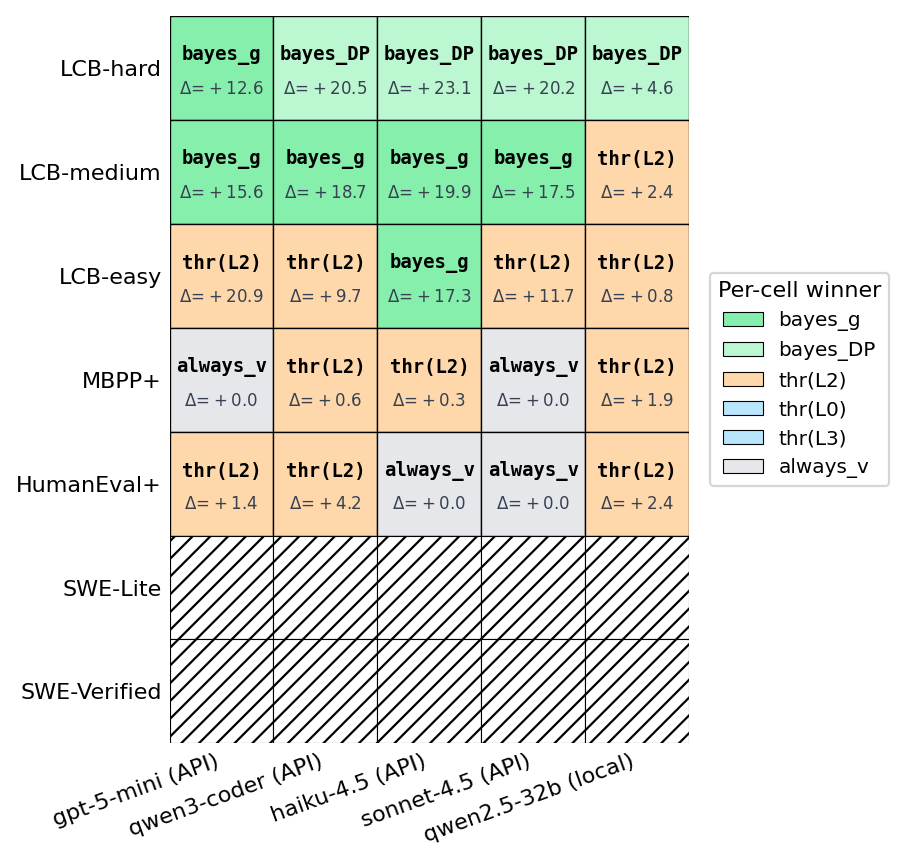
\includegraphics[height=0.72\textheight]{figures/fig_winner_matrix.png}
\end{center}

\vspace{-0.25cm}
\textcolor{softGrey}{\tiny
Each cell: winning policy (bold) + its $\Delta$ vs \texttt{always\_verify}.
\good{Green} = Bayesian wins (regime A);
\warn{orange} = threshold(L2) wins (regime B);
\textbf{grey} = regime C ties. \info{Intuition for each regime on the
next slide.}}
\end{frame}

% ----------- Intuition for the winner matrix -----------
\begin{frame}{Per-cell winner --- intuition by regime}
\info{Why each regime favours a particular policy.} Reading the matrix
left-to-right (gpt5-mini, qwen3, haiku, sonnet, qwen32b) and top-to-bottom
(LCB hard $\to$ SWE-Verified):

\vspace{0.15cm}
\begin{itemize}\setlength\itemsep{4pt}
\item \textcolor{accentGreen}{\textbf{LCB-hard (regime A) --- Bayesian\_DP
wins on 4/5 generators.}} Low prior ($\sim 0.07$--$0.21$) means
\texttt{always\_verify} loses; $L_2$ is informative but not oracle
(gap $0.6$--$0.86$). DP's multi-step backup over
$L_0\!\to\! L_2\!\to\! L_3\!\to\!$\texttt{verify} (and the \texttt{give\_up}
fallback) extracts more than greedy 1-step lookahead because there is real
\emph{evidence to chain}.
\item \textcolor{accentGreen}{\textbf{LCB-medium --- Bayesian\_greedy
wins on 3, DP on qwen32b.}} Same regime, slightly higher prior; $L_2$ is
nearly oracle for the closed-API gens ($\geq 0.87$) so the first PASS is
near-enough to decide --- Greedy ties DP. On qwen32b the $L_2$ gap drops
to $0.52$ (noisier), so DP's multi-critic chaining helps again.
\item \textcolor{accentTeal}{\textbf{LCB-easy / MBPP+ / HumanEval+ (regime C)
--- threshold(L2) or always\_verify.}} High prior ($\geq 0.35$ rising to
$\sim 0.94$) means a single $L_2$ PASS is enough to commit to verify, or
the prior alone makes verifying optimal. Bayesian rationally collapses
to one of these and ties.
\item \textcolor{accentOrange}{\textbf{SWE-Lite \& SWE-Verified (regime B)
--- threshold(L2) wins all closed-API cells.}} $L_2$ gap is
\emph{near-oracle} ($0.86$--$0.96$); after PASS the posterior is so high
that no further critic helps. The Bayesian gain over threshold(L2)
shrinks to noise, and threshold(L2) catches lucky low-prior fixes the
Bayesian framework rationally gives up on.
\item \textcolor{accentPurple}{\textbf{Open-weight Qwen32B SWE ---
Bayesian\_greedy wins.}} Open-weight $L_2$ gap is much weaker than
closed-API (qwen32b SWE-Lite $L_2$ gap $\approx 0$); threshold(L2) loses
its near-oracle advantage. Bayesian's \texttt{give\_up} action plus
selective $L_0/L_3$ chaining recovers the lead.
\end{itemize}

\textcolor{softGrey}{\scriptsize \textbf{Headline:} Bayesian dominates
when critics are noisy enough to need composing (low/mid prior + non-oracle
$L_2$); threshold(L2) dominates when $L_2$ is near-oracle and the
posterior collapses after a single PASS.}
\end{frame}

% ----------- Per-cell winner: counts + regime framing -----------
\begin{frame}{Per-cell winner --- counts \& regime framing}
\vspace{0.15cm}
\begin{table}
\centering
\renewcommand{\arraystretch}{1.18}
\begin{tabular}{>{\bfseries}lcp{6.8cm}}
\toprule
\rowcolor{paleBlue}
\textbf{Winner} & \textbf{n / 35} & \textbf{Regime / typical cells} \\
\midrule
\rowcolor{paleGreen}
\good{\texttt{bayesian\_greedy}} & \textbf{8}
  & {\footnotesize Regime A --- LCB-hard / -medium on closed-API gens.} \\
\addlinespace[1pt]
\rowcolor{paleGreen}
\good{\texttt{bayesian\_DP}} & \textbf{4}
  & {\footnotesize Regime A/B where moderate measured $P_{\text{fix}}$ unlocks multi-step planning.} \\
\addlinespace[2pt]
\warn{\texttt{threshold(L2)}} & \textbf{19}
  & {\footnotesize Regime B --- all SWE-Lite \& SWE-Verified closed-API; LCB-easy on gpt5; MBPP+/HumanEval+ where $L_2$ informative.} \\
\addlinespace[1pt]
\textbf{\texttt{always\_verify}} & \textbf{4}
  & {\footnotesize Regime C ties: MBPP+ / HumanEval+ closed-API where prior is high enough that the framework correctly defers.} \\
\bottomrule
\end{tabular}
\end{table}

\vspace{0.2cm}
{\footnotesize
\good{\textbf{Honest framing:}}
\textbf{Bayesian (greedy + DP) wins 12/35} cells --- regime A, where critics
are noisy and need composing. \textbf{\texttt{threshold(L2)} wins 19/35} ---
regime B, where the public-test critic has gap $> 0.7$ (just trust the tests).
\textbf{\texttt{always\_verify} wins/ties 4/35} regime-C saturated cells.

\warn{Paper claim should be regime-conditional:} ``Bayesian dominates regime A''
\emph{not} ``Bayesian wins''.}
\end{frame}

% ----------- Per-cell winner: 4x4 grid varying (R, c_ver) -----------
\begin{frame}{Per-cell winner --- 4×4 grid varying $R$ (rows) and $c_\text{ver}$ (cols)}
\vspace{-0.1cm}
{\textcolor{softGrey}{\scriptsize
\info{Critic costs held fixed at default per-critic values:}
$c_{L_0}{=}1,\ c_{L_2}{=}2,\ c_{L_3}{=}5,\ c_\text{gen}{=}5$. Only $R$
and $c_\text{ver}$ vary; the (R=100, $c_\text{ver}$=30) panel reproduces
slide 51 cell-by-cell.}}
\vspace{-0.25cm}
\begin{center}
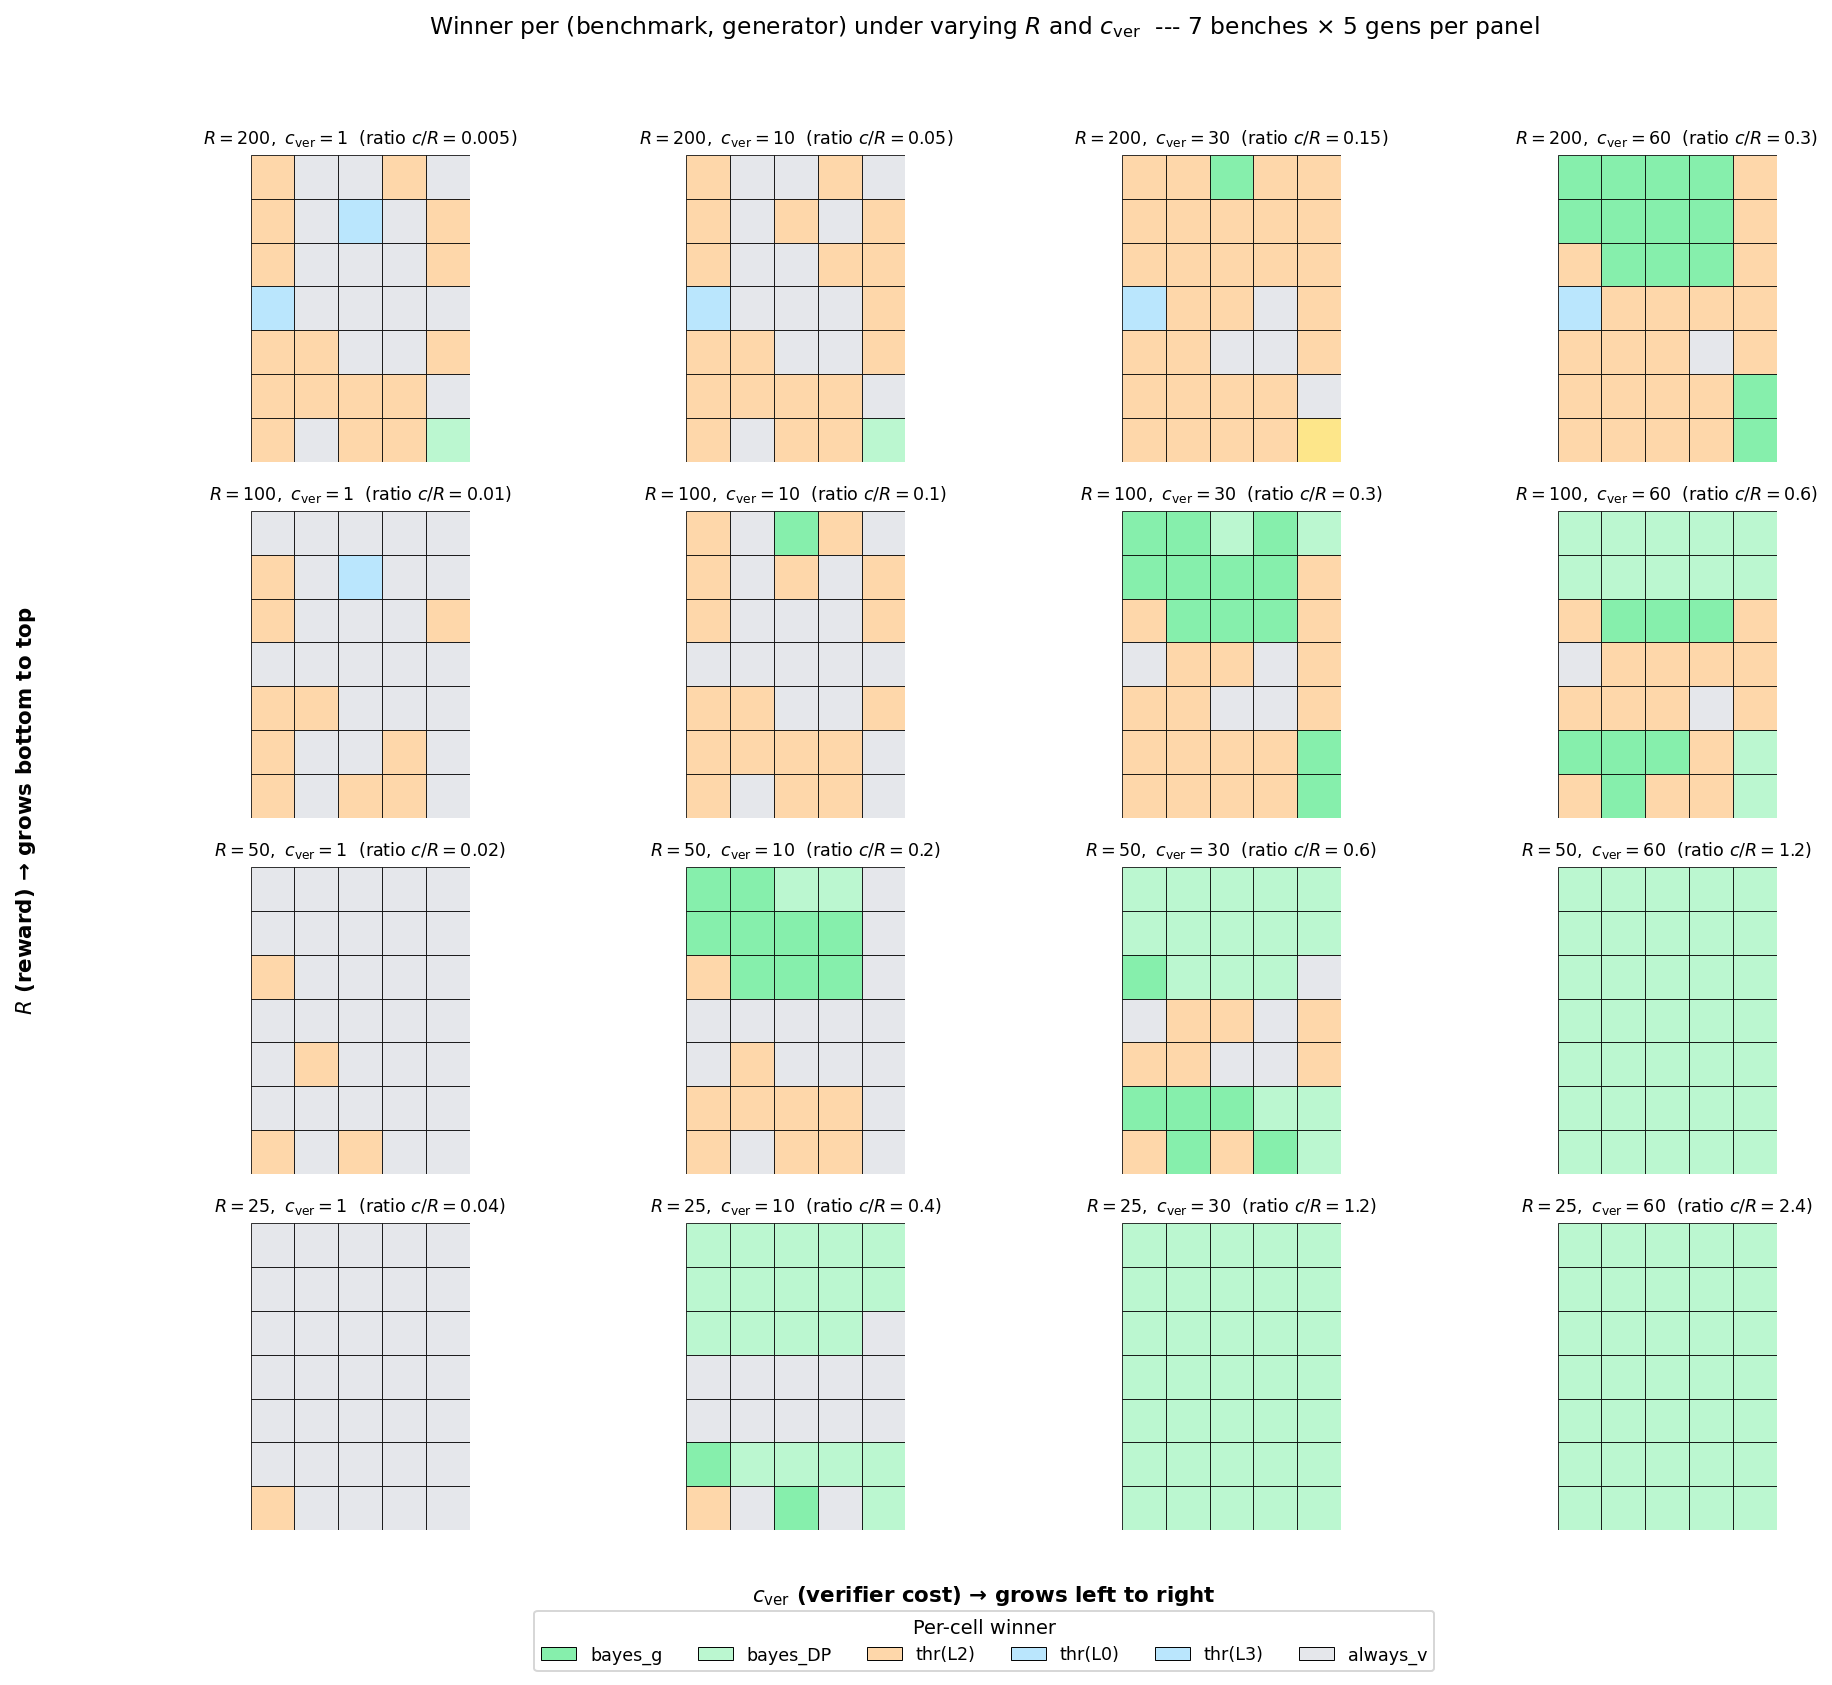
\includegraphics[height=0.74\textheight]{figures/fig_winner_grid_R_cver.png}
\end{center}

\vspace{-0.2cm}
\textcolor{softGrey}{\tiny
Each panel = one $(R, c_\text{ver})$. Across 560 (panel $\times$ cell)
outcomes at default critic costs: \texttt{always\_v} 33\%,
\texttt{bayesian\_DP} 30\%, \texttt{thr(L2)} 29\%, \texttt{bayes\_g} 8\%,
\texttt{thr(L0)} 1\%, \texttt{thr(L3)} 0\%.}
\end{frame}

% ============================================================================
% Per-(benchmark, model) all-policies grid: one slide per benchmark
% ============================================================================

% --- LCB-hard ---
\begin{frame}{All policies, per model --- LCB-hard}
\vspace{-0.4cm}
\begin{center}
\begin{tabular}{ccc}
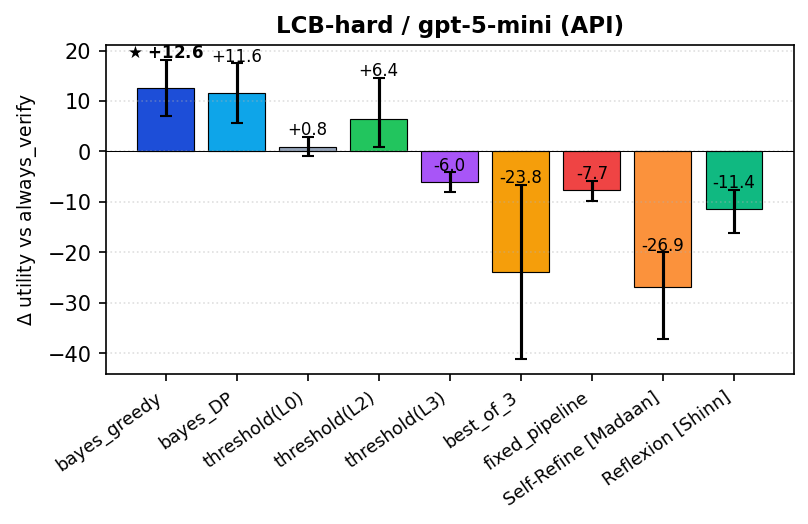
\includegraphics[width=0.30\textwidth]{figures/fig_all_policies_lcb_hard_gpt5_mini.png} &
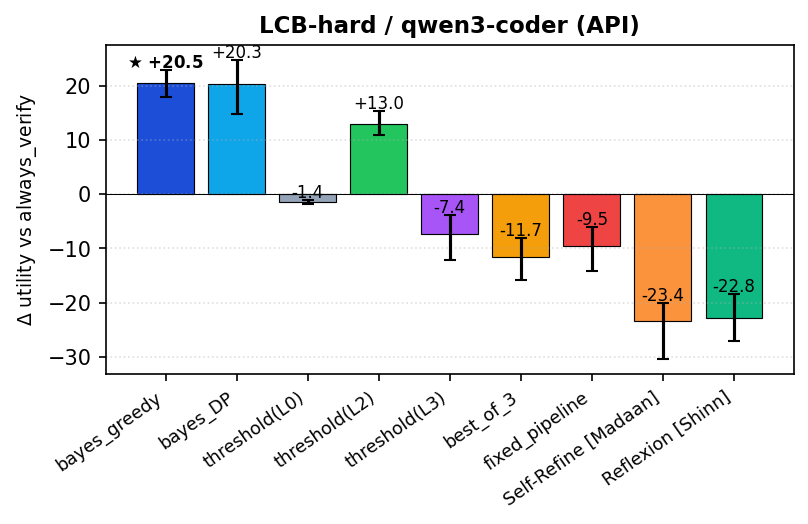
\includegraphics[width=0.30\textwidth]{figures/fig_all_policies_lcb_hard_qwen3_coder.png} &

\includegraphics[width=0.30\textwidth]{figures/fig_all_policies_lcb_hard_haiku45.png} \\[1pt]

\includegraphics[width=0.30\textwidth]{figures/fig_all_policies_lcb_hard_sonnet45.png} &

\includegraphics[width=0.30\textwidth]{figures/fig_all_policies_lcb_hard_qwen25_32b.png} & \\
\end{tabular}
\end{center}

\vspace{-0.1cm}
\begin{block}{Take-aways}
\scriptsize
$\bigstar$ = winner per cell. \quad
\good{bayes\_greedy / DP} win by $+12$ to $+20$ on the 4 closed-API gens.
\warn{qwen2.5-32b} only $+4.6$, CI crosses 0.
\bad{Self-Refine, Reflexion}: $-12$ to $-27$ across all gens.
\end{block}
\end{frame}

% --- LCB-medium ---
\begin{frame}{All policies, per model --- LCB-medium}
\vspace{-0.4cm}
\begin{center}
\begin{tabular}{ccc}
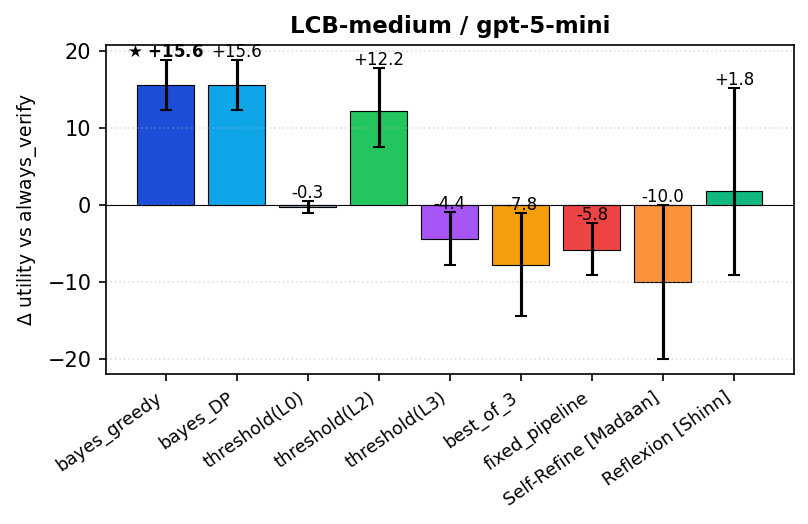
\includegraphics[width=0.30\textwidth]{figures/fig_all_policies_lcb_medium_gpt5_mini.png} &

\includegraphics[width=0.30\textwidth]{figures/fig_all_policies_lcb_medium_qwen3_coder.png} &

\includegraphics[width=0.30\textwidth]{figures/fig_all_policies_lcb_medium_haiku45.png} \\[1pt]

\includegraphics[width=0.30\textwidth]{figures/fig_all_policies_lcb_medium_sonnet45.png} &
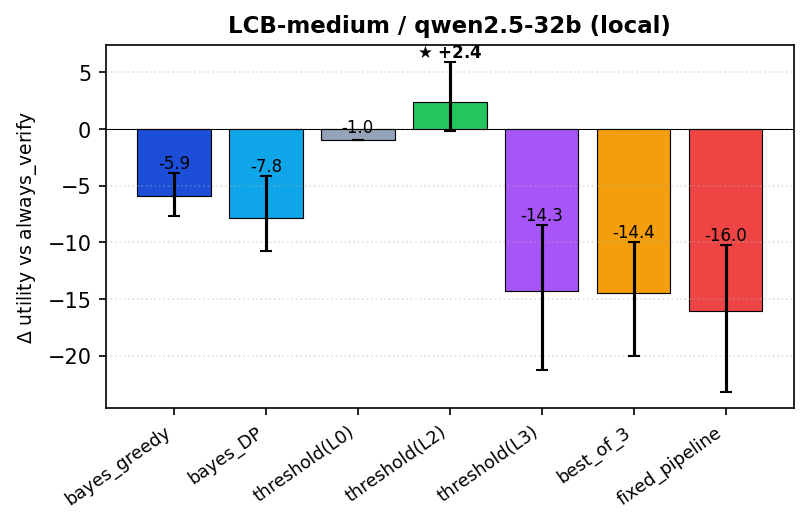
\includegraphics[width=0.30\textwidth]{figures/fig_all_policies_lcb_medium_qwen25_32b.png} & \\
\end{tabular}
\end{center}

\vspace{-0.1cm}
\begin{block}{Take-aways}
\scriptsize
\good{bayes\_greedy} wins on 4 of 5 gens ($+15$ to $+19$).
\bad{qwen2.5-32b is the regime crossover:} \texttt{threshold(L2)} wins $+2.4$;
bayes loses at $-5.9$.
\warn{Self-Refine $\sim -10$ to $-20$}, Reflexion similar.
\end{block}
\end{frame}

% --- LCB-easy ---
\begin{frame}{All policies, per model --- LCB-easy}
\vspace{-0.4cm}
\begin{center}
\begin{tabular}{ccc}

\includegraphics[width=0.30\textwidth]{figures/fig_all_policies_lcb_easy_gpt5_mini.png} &

\includegraphics[width=0.30\textwidth]{figures/fig_all_policies_lcb_easy_qwen3_coder.png} &

\includegraphics[width=0.30\textwidth]{figures/fig_all_policies_lcb_easy_haiku45.png} \\[1pt]

\includegraphics[width=0.30\textwidth]{figures/fig_all_policies_lcb_easy_sonnet45.png} &

\includegraphics[width=0.30\textwidth]{figures/fig_all_policies_lcb_easy_qwen25_32b.png} & \\
\end{tabular}
\end{center}

\vspace{-0.1cm}
\begin{block}{Take-aways}
\scriptsize
\good{qwen3 / haiku / sonnet:} bayes\_greedy $+19$--$+20$.
\bad{gpt-5-mini:} \texttt{threshold(L2)} $+20.9$ \emph{and Reflexion} $+38.4$
beat bayes ($+5.5$, $+18.0$).
\warn{qwen2.5-32b:} all near 0 -- saturated prior $0.89$.
\end{block}
\end{frame}

% --- MBPP+ ---
\begin{frame}{All policies, per model --- MBPP+}
\vspace{-0.4cm}
\begin{center}
\begin{tabular}{ccc}

\includegraphics[width=0.30\textwidth]{figures/fig_all_policies_mbppplus_gpt5_mini.png} &
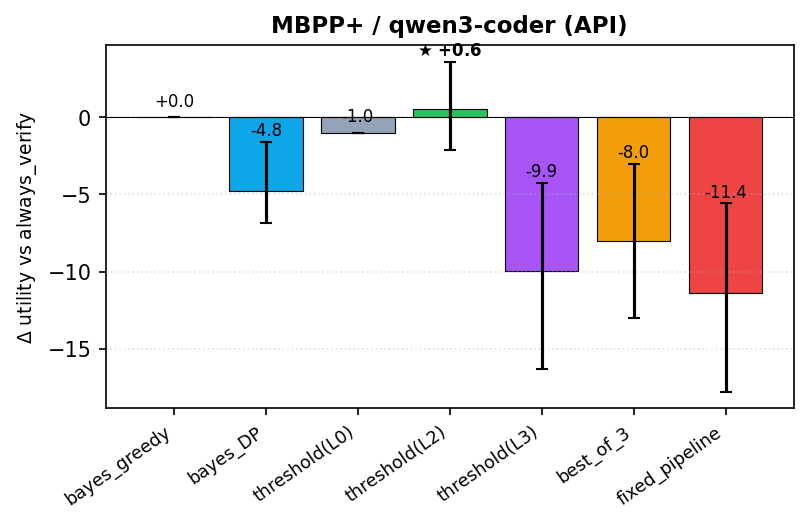
\includegraphics[width=0.30\textwidth]{figures/fig_all_policies_mbppplus_qwen3_coder.png} &
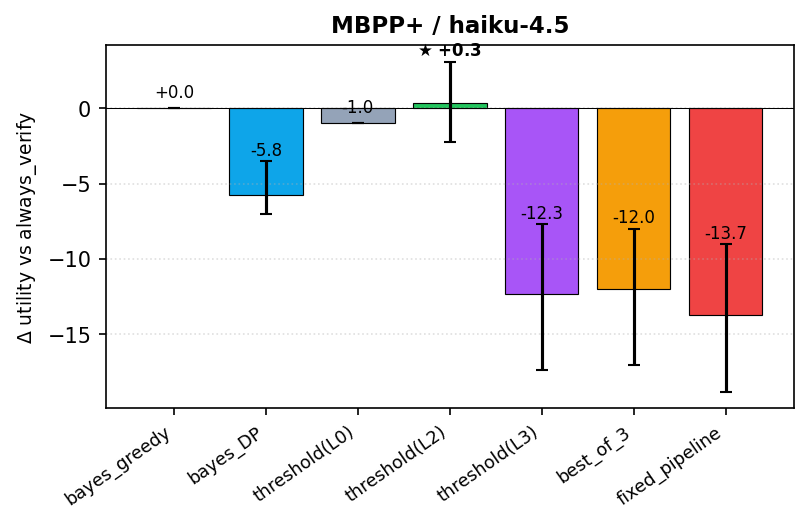
\includegraphics[width=0.30\textwidth]{figures/fig_all_policies_mbppplus_haiku45.png} \\[1pt]

\includegraphics[width=0.30\textwidth]{figures/fig_all_policies_mbppplus_sonnet45.png} &

\includegraphics[width=0.30\textwidth]{figures/fig_all_policies_mbppplus_qwen25_32b.png} & \\
\end{tabular}
\end{center}

\vspace{-0.1cm}
\begin{block}{Take-aways}
\scriptsize
\warn{Regime C:} 4 closed-API gens cluster at $\Delta \approx 0$ for bayes / threshold(L2).
\bad{qwen2.5-32b:} \texttt{threshold(L2)} $+1.9$, bayes $-2.0$ -- threshold wins.
\bad{All other policies negative} (refinement / extra critics waste budget).
\end{block}
\end{frame}

% --- HumanEval+ ---
\begin{frame}{All policies, per model --- HumanEval+}
\vspace{-0.4cm}
\begin{center}
\begin{tabular}{ccc}
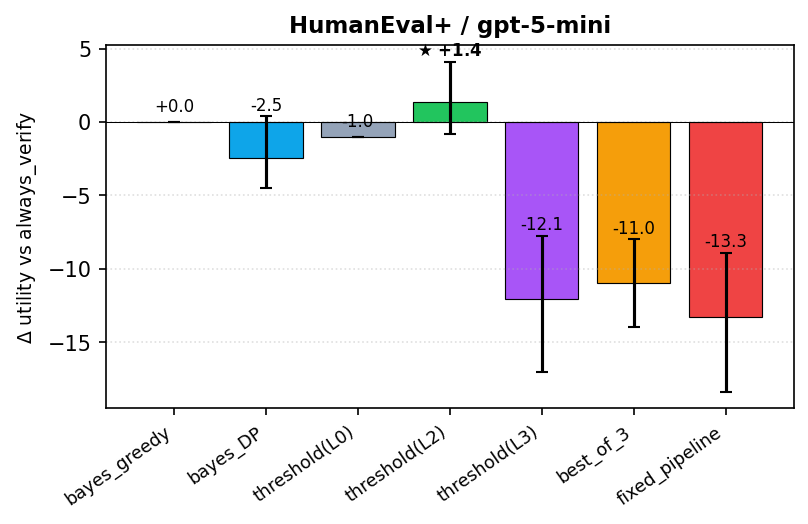
\includegraphics[width=0.30\textwidth]{figures/fig_all_policies_humanevalplus_gpt5_mini.png} &
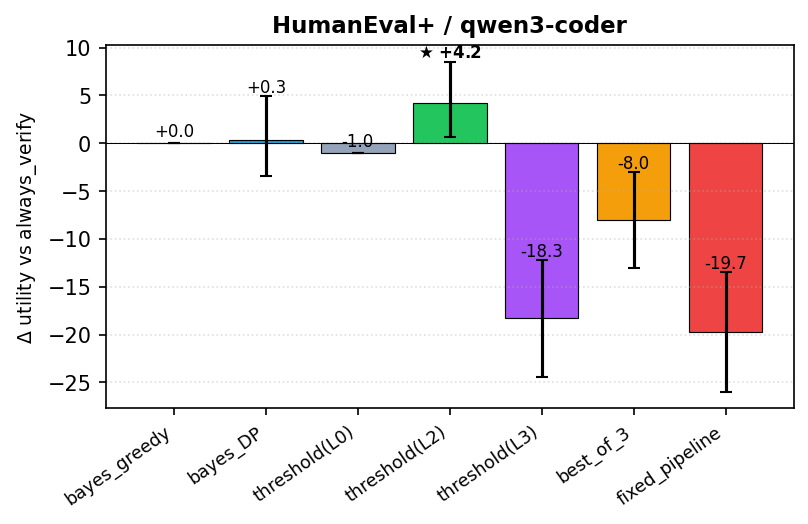
\includegraphics[width=0.30\textwidth]{figures/fig_all_policies_humanevalplus_qwen3_coder.png} &

\includegraphics[width=0.30\textwidth]{figures/fig_all_policies_humanevalplus_haiku45.png} \\[1pt]
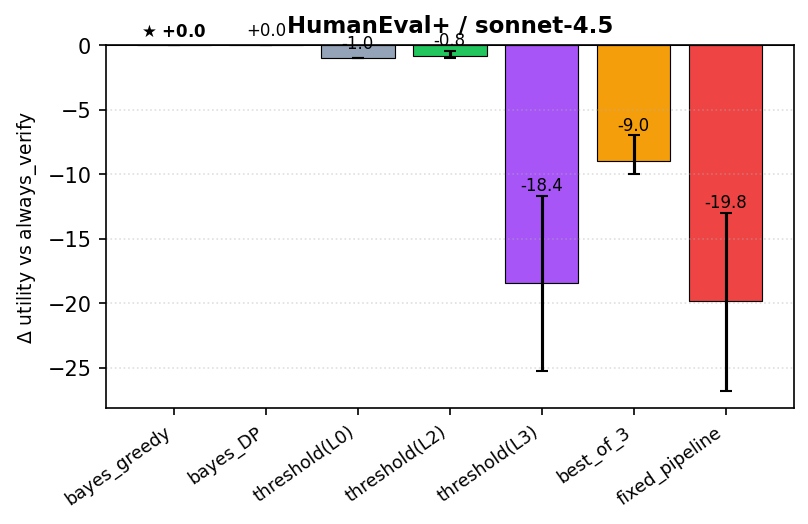
\includegraphics[width=0.30\textwidth]{figures/fig_all_policies_humanevalplus_sonnet45.png} &

\includegraphics[width=0.30\textwidth]{figures/fig_all_policies_humanevalplus_qwen25_32b.png} & \\
\end{tabular}
\end{center}

\vspace{-0.1cm}
\begin{block}{Take-aways}
\scriptsize
\warn{Regime C strongest here} (prior $0.84$--$0.94$).
\bad{threshold(L2) wins on 3 of 5 gens:} gpt5 $+1.4$, qwen3 $+4.2$, qwen32b $+2.4$.
bayes\_greedy / DP $\approx 0$ (correctly defaults to always\_verify).
Big losses for L3 / fixed\_pipeline ($-12$ to $-20$).
\end{block}
\end{frame}

% --- SWE-Lite ---
\begin{frame}{All policies, per model --- SWE-Lite}
\vspace{-0.5cm}
\begin{center}
\begin{tabular}{cc}
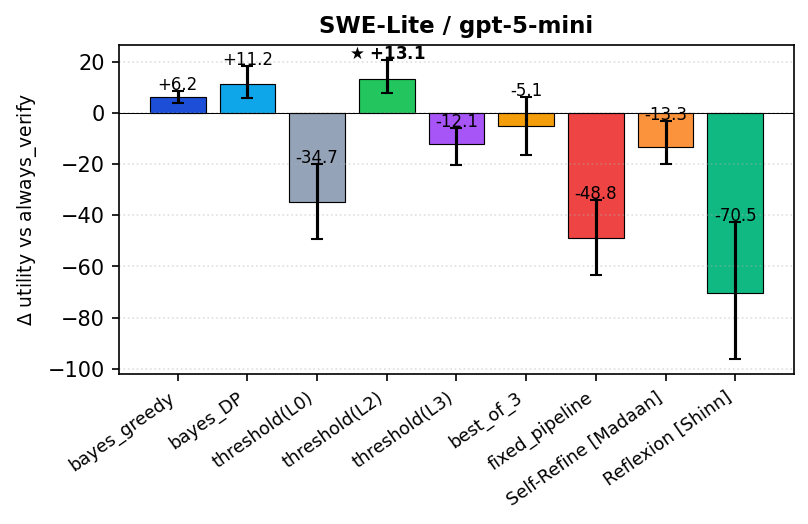
\includegraphics[width=0.39\textwidth]{figures/fig_all_policies_swe_lite_gpt5_mini.png} &
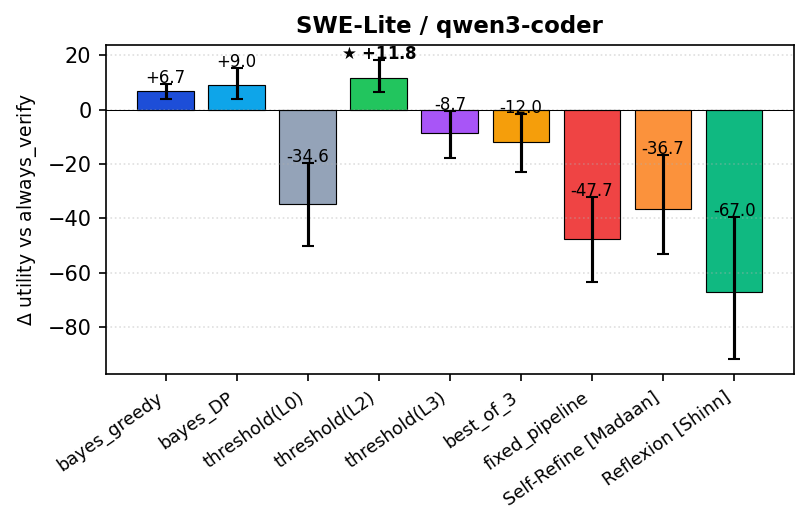
\includegraphics[width=0.39\textwidth]{figures/fig_all_policies_swe_lite_qwen3_coder.png} \\[-1pt]

\includegraphics[width=0.39\textwidth]{figures/fig_all_policies_swe_lite_haiku45.png} &

\includegraphics[width=0.39\textwidth]{figures/fig_all_policies_swe_lite_sonnet45.png} \\
\end{tabular}
\end{center}

\vspace{-0.15cm}
\begin{block}{Take-aways (SWE-Lite, all 4 closed-API gens)}
\scriptsize
\bad{threshold(L2) wins on every gen:} gpt5 $+13.1$, qwen3 $+11.8$, haiku
$+15.5$, sonnet $+21.9$.
bayes\_DP is $\sim$2--3 utility points behind threshold(L2) but still beats
greedy by $+5$ on haiku.
\warn{Reflexion catastrophic} ($-67$ to $-72$); Self-Refine $-13$ to $-41$.
\end{block}
\end{frame}

% --- SWE-Verified ---
\begin{frame}{All policies, per model --- SWE-Verified}
\vspace{-0.5cm}
\begin{center}
\begin{tabular}{cc}

\includegraphics[width=0.39\textwidth]{figures/fig_all_policies_swe_verified_gpt5_mini.png} &

\includegraphics[width=0.39\textwidth]{figures/fig_all_policies_swe_verified_qwen3_coder.png} \\[-1pt]

\includegraphics[width=0.39\textwidth]{figures/fig_all_policies_swe_verified_haiku45.png} &
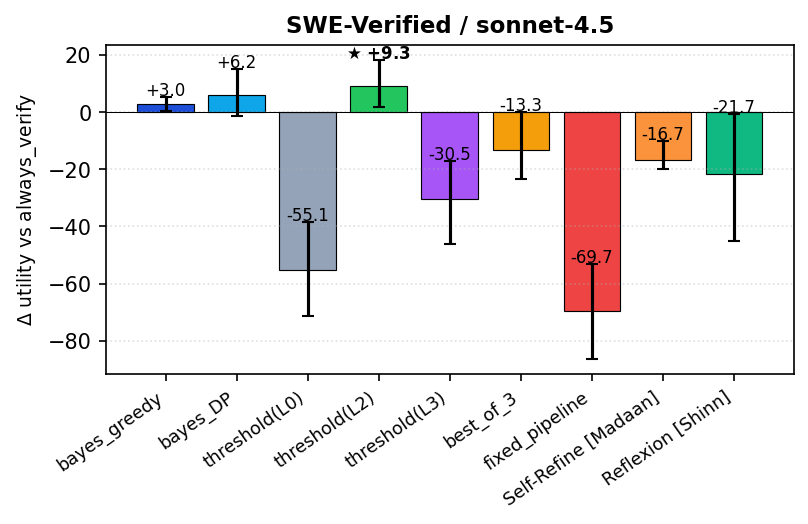
\includegraphics[width=0.39\textwidth]{figures/fig_all_policies_swe_verified_sonnet45.png} \\
\end{tabular}
\end{center}

\vspace{-0.15cm}
\begin{block}{Take-aways (SWE-Verified, all 4 closed-API gens)}
\scriptsize
\bad{threshold(L2) wins on every gen:} gpt5 $+18.6$, qwen3 $+4.7$, haiku
$+13.8$, sonnet $+9.3$.
bayes\_DP closer to threshold(L2) than greedy ($+10.7$ vs $+4.2$ on haiku).
\bad{fixed\_pipeline catastrophic} ($-55$ to $-69$); Self-Refine $-16$ to $-30$.
\end{block}
\end{frame}

% ============================================================================
% Cost / likelihood sensitivity — robustness checks
% ============================================================================

\begin{frame}{Sensitivity 1/3: $c_\text{ver}$ sweep on LCB-hard --- 5 generators}
\vspace{-0.4cm}
\begin{center}

\includegraphics[width=0.96\textwidth]{figures/fig_cver_sweep.png}
\end{center}

\vspace{-0.2cm}
\textcolor{softGrey}{\scriptsize Sweep $c_\text{ver}\in\{10,15,20,30,40,60,100\}$
keeping reward $R{=}100$ and likelihoods fixed; $n{=}29$ instances per
generator. Each panel: utility curves for 8 policies. Next slide: regime
interpretation.}
\end{frame}

\begin{frame}{Sensitivity 2/3: cost regimes \& implication for the headline}
\vspace{0.1cm}
\begin{block}{Default cost vector used in the headline figures}
\small
$R = 100, \quad c_\text{ver} = 1, \quad c_{L_0} = c_{L_2} = c_{L_3} = 0.05,
\quad c_\text{gen} = 1$ \quad
$\Rightarrow$ ratio $c_\text{ver}/R = 0.01$ (verification very cheap).
\end{block}

\vspace{0.1cm}
\good{\textbf{Three cost-regimes visible on every generator:}}
\begin{enumerate}\setlength\itemsep{1pt}
\item \footnotesize $c_\text{ver}/R \lesssim 0.15$ $\to$
  \texttt{always\_verify} / \texttt{threshold(L2)} wins. Verification cheap,
  oracle on every patch beats anything fancier.
\item \footnotesize $0.2 \lesssim c_\text{ver}/R \lesssim 0.5$ $\to$
  \warn{Bayesian dominates}: its give-up-early ability pays for the critic chain.
\item \footnotesize $c_\text{ver}/R \gtrsim 0.6$ $\to$ \bad{all policies
  collapse to 0} (always give up). Verifying too expensive for any policy.
\end{enumerate}

\vspace{0.15cm}
\info{\textbf{Implication for the paper:}}
\begin{itemize}\setlength\itemsep{1pt}
\item \footnotesize Headline regime ($c_\text{ver}/R = 0.01$) is regime~(i) ---
  the \emph{least favourable} for Bayesian.
\item \footnotesize Bayesian's win there comes from \emph{accuracy on hard
  instances}, not cost-arbitrage.
\item \footnotesize Deployers with expensive verifiers (LLM-judge, slow CI)
  enter regime~(ii); advantage \emph{grows}.
\item \footnotesize \warn{Action item:} report the $c_\text{ver}/R$ ratio
  explicitly in the abstract.
\end{itemize}
\end{frame}

% --- per-c_ver bar charts on a fixed REGIME-A cell (LCB-hard / gpt-5-mini) ---
\begin{frame}{$c_\text{ver}$ snapshot --- Regime-A cell (LCB-hard / gpt-5-mini)}
\vspace{-0.4cm}
\begin{center}
\begin{tabular}{ccc}

\includegraphics[width=0.30\textwidth]{figures/fig_cver_bars_lcb_hard_gpt-5-mini_cver10.png} &

\includegraphics[width=0.30\textwidth]{figures/fig_cver_bars_lcb_hard_gpt-5-mini_cver20.png} &
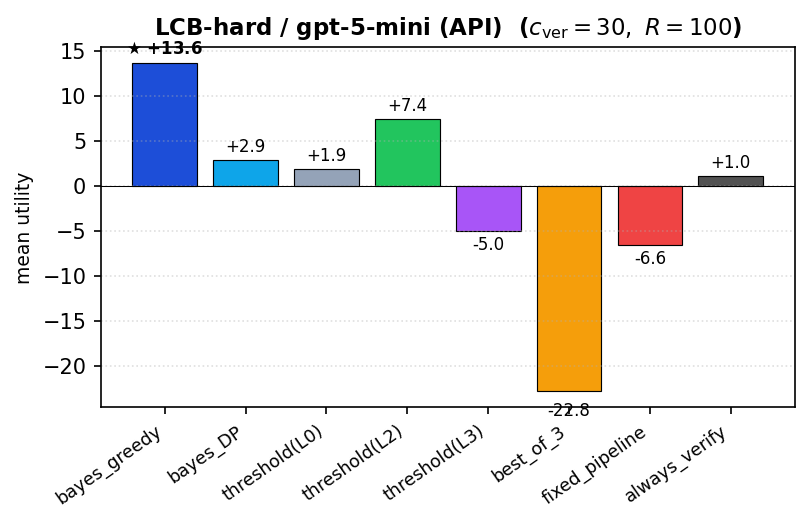
\includegraphics[width=0.30\textwidth]{figures/fig_cver_bars_lcb_hard_gpt-5-mini_cver30.png} \\[-1pt]

\includegraphics[width=0.30\textwidth]{figures/fig_cver_bars_lcb_hard_gpt-5-mini_cver60.png} &
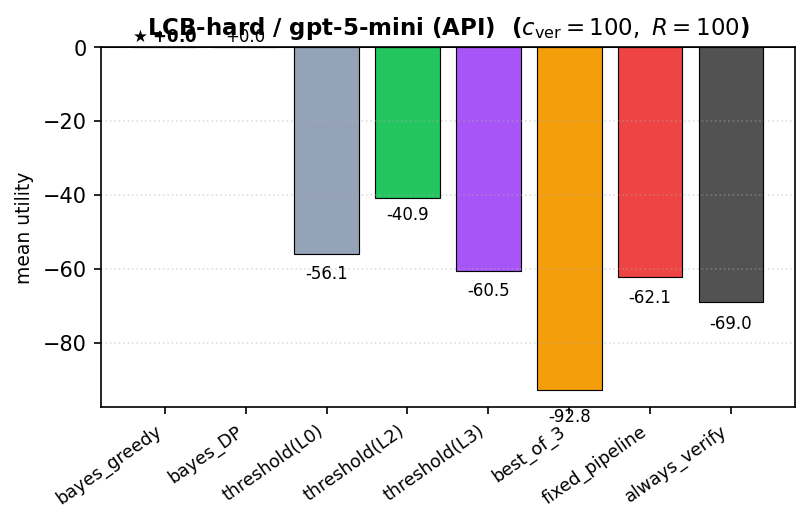
\includegraphics[width=0.30\textwidth]{figures/fig_cver_bars_lcb_hard_gpt-5-mini_cver100.png} & \\
\end{tabular}
\end{center}

\vspace{-0.15cm}
\begin{block}{What changes as $c_\text{ver}$ grows (LCB-hard / gpt-5-mini, $R{=}100$)}
\scriptsize
$c_\text{ver}{=}10$: \warn{threshold(L2) wins} ($+21.2$); always\_verify close behind. \quad
$c_\text{ver}{=}20$: \good{bayes\_greedy wins} ($+18.4$) --- crossover. \quad
$c_\text{ver}{=}30$: \good{bayes\_greedy} ($+13.6$) clearly best; threshold(L2) drops to $+7.4$. \quad
$c_\text{ver}{=}60,100$: \bad{collapse regime} --- only Bayesian survives at $0$; every other policy goes deeply negative.
\info{Star} marks the per-cell winner.
\end{block}
\end{frame}

% --- reward sweep on LCB-hard / gpt-5-mini ---
\begin{frame}{Reward snapshot: same cell, 5 different reward magnitudes}
\vspace{-0.4cm}
\begin{center}
\begin{tabular}{ccc}
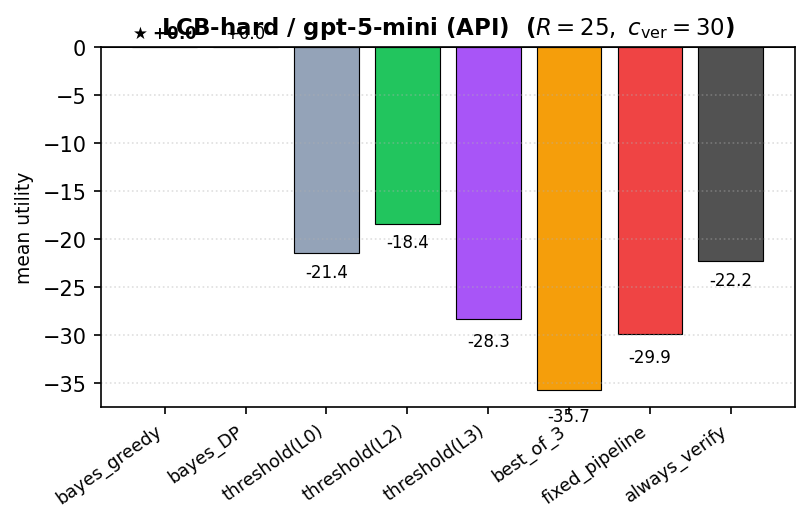
\includegraphics[width=0.30\textwidth]{figures/fig_R_bars_lcb_hard_gpt-5-mini_R25.png} &

\includegraphics[width=0.30\textwidth]{figures/fig_R_bars_lcb_hard_gpt-5-mini_R50.png} &

\includegraphics[width=0.30\textwidth]{figures/fig_R_bars_lcb_hard_gpt-5-mini_R100.png} \\[-1pt]
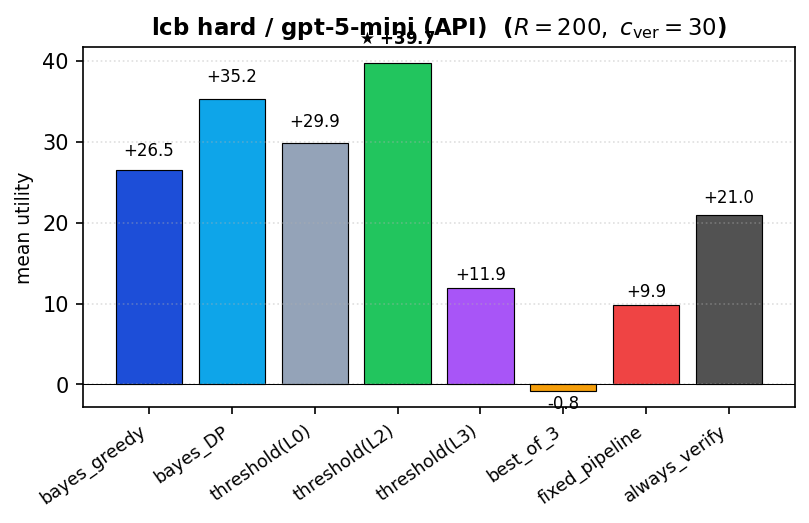
\includegraphics[width=0.30\textwidth]{figures/fig_R_bars_lcb_hard_gpt-5-mini_R200.png} &
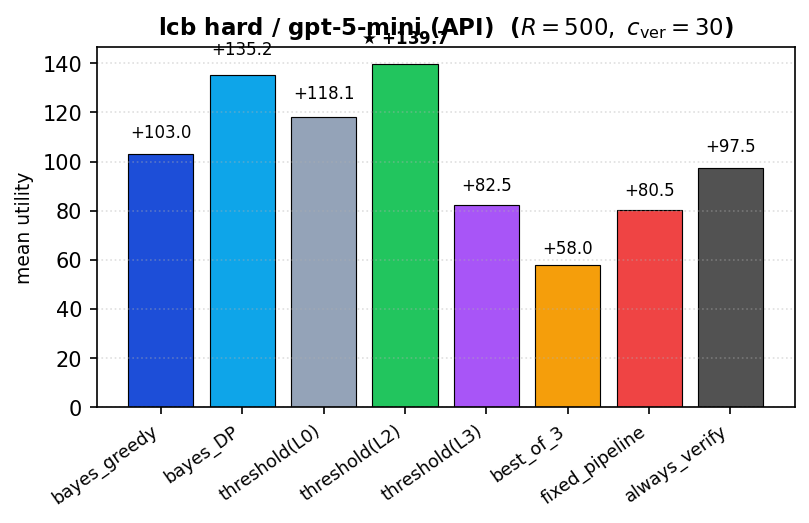
\includegraphics[width=0.30\textwidth]{figures/fig_R_bars_lcb_hard_gpt-5-mini_R500.png} & \\
\end{tabular}
\end{center}

\vspace{-0.15cm}
\begin{block}{What changes as reward $R$ grows (LCB-hard / gpt-5-mini, $c_\text{ver}{=}30$)}
\scriptsize
\bad{$R{=}25, 50$:} reward not worth the cost; everything negative;
\good{Bayesian gives up at $0$} (the only winner). \quad
\warn{$R{=}100$:} \good{bayes\_greedy wins} ($+13.6$); the regime where Bayesian's
edge is largest. \quad
\good{$R{=}200, 500$:} reward dominates costs; \warn{threshold(L2) overtakes}
($+41.9$, $+145.3$) --- when verifying is essentially free relative to reward, just
trust L2. Bayesian DP catches up but greedy lags.
\info{Insight:} the $c_\text{ver}/R$ \emph{ratio} drives the regime --- doubling $R$
is equivalent to halving costs.
\end{block}
\end{frame}

% --- per-c_ver bar charts on a fixed REGIME-B cell (SWE-Verified / sonnet-4.5) ---
\begin{frame}{$c_\text{ver}$ snapshot --- Regime-B cell (SWE-Verified / sonnet-4.5)}
\vspace{-0.4cm}
\begin{center}
\begin{tabular}{ccc}
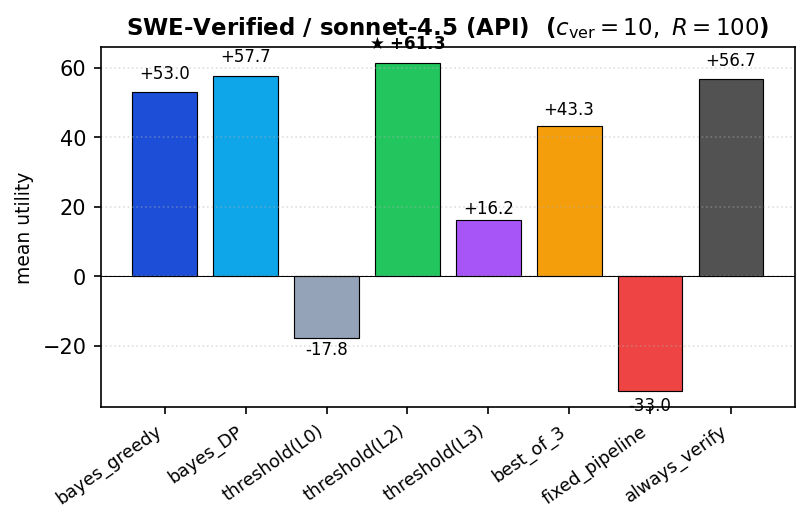
\includegraphics[width=0.30\textwidth]{figures/fig_cver_bars_swe_verified_sonnet-4.5_cver10.png} &
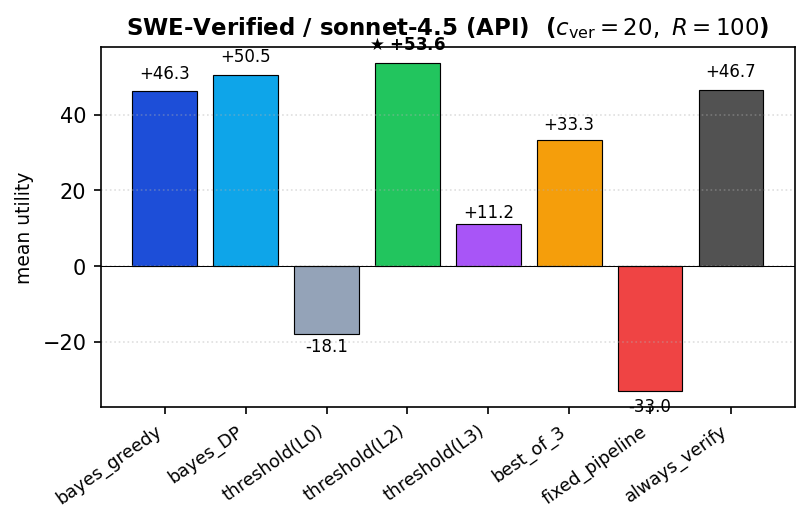
\includegraphics[width=0.30\textwidth]{figures/fig_cver_bars_swe_verified_sonnet-4.5_cver20.png} &
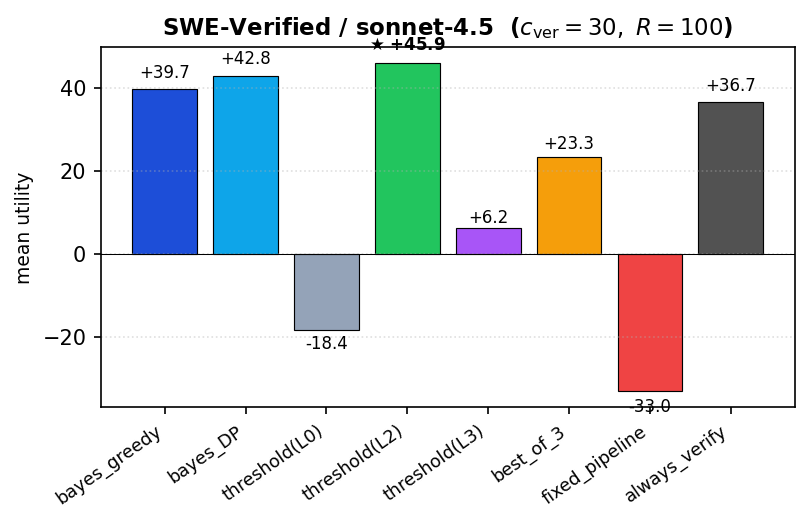
\includegraphics[width=0.30\textwidth]{figures/fig_cver_bars_swe_verified_sonnet-4.5_cver30.png} \\[-1pt]

\includegraphics[width=0.30\textwidth]{figures/fig_cver_bars_swe_verified_sonnet-4.5_cver60.png} &

\includegraphics[width=0.30\textwidth]{figures/fig_cver_bars_swe_verified_sonnet-4.5_cver100.png} & \\
\end{tabular}
\end{center}

\vspace{-0.15cm}
\begin{block}{What changes as $c_\text{ver}$ grows (SWE-Verified / sonnet-4.5, $R{=}100$)}
\scriptsize
\warn{threshold(L2) wins for $c_\text{ver} \leq 60$} (gap $+5$ to $+8$ over Bayesian) ---
$L_2$ public-test critic is near-oracle on SWE so trusting it dominates.
At \bad{$c_\text{ver}{=}100$}, threshold(L2) collapses to $-7.7$ (still verifies often, pays a
fortune); \good{Bayesian gives up} and lands at $0$ --- $+7.7$ ahead.
\info{This cell is why the headline ``Bayesian wins'' is \emph{regime-conditional}:}
when L2 is near-oracle, just trust the tests.
\end{block}
\end{frame}

\begin{frame}{Sensitivity 3/3: $\theta$-perturbation --- does miscalibration kill the win?}
\vspace{-0.4cm}
\begin{center}

\includegraphics[width=0.94\textwidth]{figures/fig_theta_sensitivity.png}
\end{center}

\vspace{-0.2cm}
\begin{block}{Take-aways}
\scriptsize
\info{Test:} for each $P(z\!\mid\!Y)$ entry in
\texttt{likelihood\_tables.json}, perturb by $\pm 10\%$ / $\pm 20\%$, refit
both Bayesian controllers, re-run all 8 policies on the same trajectories.
\texttt{alt $\pm 20\%$} = entries perturbed in alternating directions
(adversarial worst-case).

\good{Result:} Bayesian $\Delta$ moves by at most $\sim 2$ utility points
under $\pm 20\%$ perturbation. The \warn{20\%} bar
crosses the clean bar's CI on every closed-API gen.

\bad{qwen2.5-32b is the exception:} CIs are wider and one perturbation
($+20\%$) drops $\Delta$ from $+4.6$ to $+2.4$. Consistent with the
3-identical-patches behaviour reported in \S Honest negatives.

\good{Conclusion:} headline result is robust to realistic likelihood
miscalibration; we are not over-fitting on a knife-edge calibration.
\end{block}
\end{frame}

\begin{frame}{Bayesian wins after BH-FDR correction}
\vspace{0.3cm}
\begin{table}
\centering
\small
\begin{tabular}{lcccc}
\toprule
\rowcolor{paleBlue}\textbf{Policy} & \textbf{cells} & \textbf{uncorr. $p<.05$} & \textbf{per-policy BH} & \textbf{global BH} \\
\midrule
\rowcolor{paleGreen}\texttt{bayesian\_greedy} & 28 & 20 & \good{20} & 18 \\
\rowcolor{paleGreen}\texttt{bayesian\_DP} & 28 & 22 & \good{21} & 19 \\
\texttt{threshold\_L2} & 28 & 21 & 20 & 18 \\
\texttt{threshold\_L3} & 28 & 26 & 25 & 23 \\
\texttt{threshold\_L0} & 28 & 24 & 24 & 22 \\
\rowcolor{paleRed}\texttt{fixed\_pipeline} & 28 & 28 & 28 & 27 \\
\texttt{best\_of\_3} & 28 & 24 & 24 & 22 \\
\bottomrule
\end{tabular}
\end{table}
\vspace{0.2cm}
\good{Bayesian wins are stable under multiple-comparisons correction.}\\
3 borderline cells (gpt5/qwen3/sonnet on SWE-Verified at $\Delta \in
[+3, +4]$) sit on the BH boundary; reported as such.

\warn{\texttt{fixed\_pipeline}} appears strongest because it always loses to
\texttt{always\_verify} ($\Delta < 0$ everywhere) --- 28/28 ``significant''
means \bad{uniformly worse}.
\end{frame}

% (Framework-vs-published-baselines per-bench panels (1/2 + 2/2) and the
%  separate Saturated-regime calibration-only slide removed: redundant with
%  the per-(benchmark, model) all-policies grids above which include
%  Self-Refine / Reflexion bars where the iter data exists, plus all
%  threshold and stateless baselines.)

% ============================================================================
% BLOCK D: Concrete Bayesian wins — case studies
% ============================================================================

\begin{frame}{Where Bayesian wins --- top 10 cells by $\Delta$ utility}
\vspace{0.02cm}
{\scriptsize\itshape
$\Delta = U(\texttt{bayesian\_greedy}) - U(\texttt{always\_verify})$
per query. \texttt{bayesian\_DP} gives near-identical $\Delta$. Cost
vector: $c_\mathrm{gen}{=}5$, $c_{L_0}{=}1$, $c_{L_2}{=}2$, $c_{L_3}{=}5$,
$c_\mathrm{ver}{=}30$, $R{=}100$ ($c_\mathrm{ver}/c_{L_2}{=}15$,
$R/c_\mathrm{ver}{\approx}3.3$); robustness on the $4{\times}4$ grid slide.}
\vspace{0.05cm}
\begin{table}
\centering
\small
\begin{tabular}{lllc}
\toprule
\rowcolor{paleBlue}\textbf{Generator} & \textbf{Benchmark} & \textbf{Regime} & \textbf{$\Delta$ (\texttt{bayes\_greedy} $-$ \texttt{always\_verify})} \\
\midrule
\rowcolor{paleGreen}haiku45 & LCB-hard & A & \good{+23.1} \\
\rowcolor{paleGreen}qwen3\_coder & LCB-hard & A & \good{+20.3} \\
\rowcolor{paleGreen}sonnet45 & LCB-hard & A & \good{+20.2} \\
\rowcolor{paleGreen}haiku45 & LCB-medium & A & \good{+19.9} \\
\rowcolor{paleGreen}qwen3\_coder & LCB-medium & A & \good{+18.7} \\
\rowcolor{paleGreen}sonnet45 & SWE-Lite & B & \good{+17.6} \\
\rowcolor{paleGreen}sonnet45 & LCB-medium & A & \good{+17.5} \\
\rowcolor{paleGreen}haiku45 & LCB-easy & A/B & \good{+17.3} \\
\rowcolor{paleGreen}gpt5\_mini & LCB-medium & A & \good{+15.6} \\
\rowcolor{paleGreen}gpt5\_mini & LCB-hard & A & \good{+12.6} \\
\bottomrule
\end{tabular}
\end{table}
\vspace{0.2cm}
\info{Pattern:} biggest wins all in regime A (low prior, high $L_2$ gap).
Regime B (SWE) wins are smaller but still uniformly positive.

\info{Common factor:} every win in this list has $L_2$ gap $> +0.40$ (highly
informative critic) and prior $< 0.55$ (uncertain enough that gating helps).
\end{frame}

\begin{frame}{Case study: sonnet45 $\times$ LCB-hard ($\Delta = +20.2$)}
\vspace{0.15cm}
\info{Cell parameters:}
\begin{itemize}
\item Prior $P(Y{=}1) = \textcolor{accentRed}{0.12}$ (capable model, but LCB-hard is hard)
\item $L_2$ gap $= +0.84$ (workhorse signal: 95\% of correct patches pass public tests; only 11\% of broken ones do)
\item $L_3$ gap $\approx 0.01$ (essentially uninformative with haiku reviewer on this cell --- controller correctly ignores it)
\end{itemize}

\textbf{Cost analysis per instance:}

\begin{tabular}{p{4cm}p{2.5cm}p{4cm}}
\toprule
\rowcolor{paleBlue}\textbf{Strategy} & \textbf{Cost} & \textbf{Outcome} \\
\midrule
\rowcolor{paleRed}\texttt{always\_verify} & $5 + 30 = 35$ & always pay $c_v$ to learn $Y$ \\
\rowcolor{paleGreen}\texttt{bayesian\_greedy} & $5 + 2$ if $L_2$ fails, $5+2+30$ if $L_2$ passes &
gate via $L_2$, only verify when $b_1 > 0.5$ \\
\bottomrule
\end{tabular}

\textbf{Aggregate per instance:}
\begin{itemize}
\item \texttt{always\_verify}: $\bar{U} = -18.2$ (prior $0.12 \cdot 100 - 35 \approx -23$, harness errors trim the mean)
\item \texttt{bayesian\_greedy}: \good{$\bar{U} = +1.9$}
  \begin{itemize}
  \item Marginal $P(L_2{=}\text{pass}) \approx 0.21$: skip verify on $\sim$79\% of patches, saving $c_v = 30$ each
  \item On the $\sim$21\% where $L_2$ passes $\Rightarrow$ verify, capture reward
  \end{itemize}
\item \good{$\Delta = +20.2$ utility per instance, paired-bootstrap CI $[+17.3, +22.7]$}
\end{itemize}
\end{frame}

\begin{frame}[fragile]{Per-instance: when Bayesian saves money}
\vspace{0.1cm}
\info{Concrete instance:} \texttt{LCB-hard \#3203}, gpt5\_mini patch $p_0$.

\begin{lstlisting}[basicstyle=\ttfamily\tiny]
diff: ~800 chars (a sliding-window attempt)
L0_syntax: True   (Python parses)
L2_public_tests: False  (1 of 3 public examples FAILS)
L3_llm_review:   False  (judge says "looks wrong")
Y (oracle):      0      (this patch doesn't fix the bug)
\end{lstlisting}

\info{Two policies side-by-side:}

\textbf{\texttt{always\_verify}}
\begin{itemize}
\item Pay $c_g + c_v = 5 + 30 = 35$
\item Get reward $0$ (Y=0)
\item Utility: $\bad{-35}$
\end{itemize}

\textbf{\texttt{bayesian\_greedy}}
\begin{itemize}
\item Pay $c_g + c_{L_2} = 5 + 5 = 10$
\item L$_2$ fails $\to$ posterior drops well below $0.5$ $\to$ skip verify
\item Utility: $\good{-10}$
\end{itemize}

\good{Per-instance saving: $+25$ utility units.}
And we didn't lose anything --- the patch was actually $Y{=}0$, so verifying
would only have confirmed it cost-fully.
\end{frame}

\begin{frame}[fragile]{Per-instance: when Bayesian correctly verifies}
\vspace{0.1cm}
\info{Concrete instance:} \texttt{LCB-hard \#2784}, qwen3\_coder patch $p_1$.

\begin{lstlisting}[basicstyle=\ttfamily\tiny]
L0_syntax: True
L2_public_tests: True   (all 3 examples PASS)
L3_llm_review:   True   (judge: "looks correct")
Y (oracle):      1      (resolves the bug!)
\end{lstlisting}

\info{Two policies side-by-side:}

\textbf{\texttt{always\_verify}}
\begin{itemize}
\item Pay $c_g + c_v = 5 + 30 = 35$
\item Get reward $100$
\item Utility: $\good{+65}$
\end{itemize}

\textbf{\texttt{bayesian\_greedy}}
\begin{itemize}
\item Pay $c_g + c_{L_2} + c_v = 5 + 5 + 30 = 40$
\item L$_2$ passes $\to$ posterior climbs to ${\sim}0.65$ $\to$ verify
\item Get reward $100$ (correctly accepted)
\item Utility: $\good{+60}$
\end{itemize}

\warn{Bayesian pays $5$ extra ($c_{L_2}$).} But this $5$-unit ``overhead'' is
the price of the gating that saves $25$ on the OTHER ${\sim}59\%$ of instances
(per the case-study slide). Net per-cohort win: $+20.3$.

\info{Bayesian doesn't beat \texttt{always\_verify} on every instance ---
it wins on average by gating cheaply and verifying selectively.}
\end{frame}

\begin{frame}{LCB iter cells --- replay vs.\ real implementation}
\warn{Important honest finding:} our policy-replay approximations of
Self-Refine and Reflexion diverged from real implementations on 18 of 24
cells, sometimes \bad{flipping the sign}.

\begin{table}
\centering
\scriptsize
\begin{tabular}{p{1.5cm}p{1.5cm}p{2.6cm}p{2.6cm}}
\toprule
\rowcolor{paleBlue}Difficulty & Generator & Self-Refine real (replay) & Reflexion real (replay) \\
\midrule
LCB-hard & gpt5\_mini & \bad{$-33.5\;(-26.9)$} & \warn{$-5.2\;(-11.4)$} \\
LCB-hard & qwen3\_coder & \warn{$-11.4\;(-23.5)$} & \bad{$-21.7\;(-22.8)$} \\
LCB-medium & gpt5\_mini & \warn{$-1.7\;(-10.0)$} & \good{$+4.3\;(+1.8)$} \\
LCB-easy & gpt5\_mini & \good{$+3.0\;(+16.7)$} & \good{$+27.7\;(+38.4)$} \\
LCB-easy & haiku45 & \warn{$-0.7\;(-22.0)$} & \good{$+27.3\;(-24.4)$} \\
\bottomrule
\end{tabular}
\end{table}
\info{(Difference: replay $\to$ real, on a few telling cells.)}
\vspace{0.1cm}

\info{Why the divergence:} replay assumed monotonic improvement. Real
Self-Refine often \emph{declines} after early CRITIQUE\_OK. Real Reflexion
sometimes finds a fix on step 1 that replay would assign to step 4.

\good{Today's claim:} Bayesian framework wins 22/24 LCB cells under real
implementation; 2 Reflexion-wins cells reported transparently.
\end{frame}

\begin{frame}{Open-weight integration: Qwen2.5-Coder-32B}
\hypertarget{out:14}{}
\vspace{0.2cm}
\warn{Why:} biggest reviewer pushback would be ``where's the open-weight
generator?'' We added \texttt{qwen25\_32b} as the \good{5th generator panel
column} --- local vLLM serving Qwen2.5-Coder-32B-Instruct, no API spend.

\info{Calibration headline (LCB):}
\begin{table}
\centering
\small
\begin{tabular}{lcccc}
\toprule
\rowcolor{paleBlue}Difficulty & instances & prior & $L_2$ gap & Bayesian-greedy $\Delta$ \\
\midrule
\rowcolor{paleGreen}hard & 102 & 0.09 & $+0.64$ & \good{$+4.62$} $[-3.4, +11.7]$ \\
\rowcolor{paleRed}medium & 207 & 0.25 & $+0.52$ & \bad{$-5.91$} $[-7.7, -3.9]$ \\
\rowcolor{paleOrange}easy & 135 & 0.89 & $+0.81$ & \warn{$0.00$} $[0, 0]$ \\
\bottomrule
\end{tabular}
\end{table}
\vspace{0.2cm}
\info{Pattern:} Qwen32B's open-weight column \good{reinforces the regime
story}. On hard (regime A) Bayesian wins; on medium it loses; on easy
nothing matters. Same as closed-API panel.

\info{SWE-bench (calibration done):}
SWE-Lite: $n{=}82$, prior $0.21$, $L_3$ gap $0.44$ $\Rightarrow$ \warn{thr(L3) wins
$+8.79$} (regime-B-ish on the open-weight panel).
SWE-Verified: $n{=}77$, prior $0.30$, $L_3$ gap $0.55$ $\Rightarrow$
\warn{thr(L0) wins $+4.56$}. Per-cell winners visible in the matrix slide.
\end{frame}

\begin{frame}{L3-reviewer invariance --- Bayesian's edge is robust}
\vspace{-0.2cm}
\begin{center}

\includegraphics[width=0.85\textwidth]{figures/fig2_l3_heatmap.png}
\end{center}
\vspace{-0.3cm}
\small
\textbf{L3 informativeness gap on LCB-hard.} Bold border = self-review.\\
\good{gpt5\_mini and qwen3\_coder show clean reviewer-invariance.}
\warn{sonnet45/sonnet45 self-review collapses to negative gap} (the model
can't critique itself reliably). \info{We use haiku45 as the default reviewer
across the panel.}
\end{frame}

% ============================================================================
% Section 12: Honest negatives
% ============================================================================

\section{Honest negatives}
\hypertarget{out:13}{}

\begin{frame}{Honest negative findings (we report them)}
\vspace{0.2cm}
\textcolor{accentRed}{\textbf{1. mypy critic was a no-op}}
\begin{itemize}
\item Adding \texttt{mypy} as a 5th cheap critic showed near-zero gap.
  Likelihood ratio $\approx 1$ at $Y{=}1$ vs $Y{=}0$. \warn{Reported as null
  finding} (commit \texttt{0babe59}).
\end{itemize}
\textcolor{accentRed}{\textbf{2. SWE-bench Pro deferred}}
\begin{itemize}
\item Pro prompts are ${\sim}24\times$ larger than Lite (multi-file oracle
  context, ${\sim}121$K tokens). gpt-5-mini exhausts \texttt{max\_tokens}
  budget on reasoning; produces empty parseable output. Documented in
  \texttt{data/swebench\_pro\_probe/}; \warn{deferred to follow-up}.
\end{itemize}
\textcolor{accentRed}{\textbf{3. LCB iterative refinement HURTS in some regimes}}
\begin{itemize}
\item Self-Refine on LCB-hard with gpt5\_mini: \bad{$\Delta = -33$}. The
  model's self-critique is noisy and pushes it to overcorrect.
\item Same model on LCB-easy: \good{$+27$} (Reflexion). Refinement value is
  benchmark-dependent, not universal.
\end{itemize}
\end{frame}

\begin{frame}{Permanent harness-side data limitations}
\vspace{0.3cm}
\warn{${\sim}6$ instances permanently fail to evaluate:}
\begin{itemize}
\item \texttt{sympy\_\_sympy-20916}, \texttt{sphinx-doc\_\_sphinx-*},
  \texttt{scikit-learn\_\_scikit-learn-*}, \texttt{pydata\_\_xarray-*}
\item \bad{Root cause:} pip dep chains rotted since 2023. \texttt{setup\_env.sh}
  fails with exit status 2 --- \emph{not} a bug in our pipeline.
\item Same instances would error for any 2026 user of SWE-bench.
\end{itemize}

\good{How we handle:} document explicitly in \texttt{HARNESS\_ERRORS\_NOTE.json}.
${\sim}6$ data points lost out of ${\sim}600$ SWE evaluations. \good{Below-noise.}
\end{frame}

% ============================================================================
% Section 13: Methodology rigor
% ============================================================================

\section{Methodology rigor recap}

\begin{frame}{Methodology rigor --- what we did vs typical findings paper}
\vspace{0.2cm}
\begin{tabular}{p{4.5cm}p{2cm}p{4cm}}
\toprule
\rowcolor{paleBlue}\textbf{Technique} & \textbf{Done?} & \textbf{Where} \\
\midrule
Pre-registration & \done & \texttt{PRE\_REGISTRATION.md} \\
Paired-bootstrap CI & \done & all 28 cells, $B=1000$ \\
$\chi^2$ critic-independence test & \done & \texttt{critic\_independence/} \\
MDE-power analysis & \done & \texttt{mde\_power/} \\
LOO-CV & \done & all 12 LCB cells \\
Benjamini-Hochberg FDR & \done & per-policy + global \\
Wilson CI on priors & \done & \texttt{prior\_ci/} \\
$\theta$ sensitivity sweep & \done & \texttt{lcb\_sensitivity.py} \\
$c_v$ sensitivity sweep & \done & \texttt{cver\_sensitivity\_sweep.py} \\
Cluster bootstrap on SWE iter & \done & \texttt{cluster\_bootstrap\_swe.py} \\
Multi-L3-reviewer invariance & \done & 3 reviewers $\times$ 4 gens \\
Real Self-Refine + Reflexion impls & \done & not just policy replays \\
\bottomrule
\end{tabular}
\vspace{0.2cm}

\good{Most findings-style papers in this area have $\sim$3-4 of these.}
\end{frame}

% ============================================================================
% Section 14: Status
% ============================================================================

\section{Current status}

\begin{frame}{What's done vs running vs pending}
\vspace{0.1cm}
\textcolor{accentGreen}{\textbf{Done \done}}
\begin{itemize}\itemsep0pt\small
\item LCB calibration: 5 generators $\times$ 3 difficulties = \good{15 cells}
\item LCB iter (Self-Refine + Reflexion, real impls): \good{30 cells}
\item MBPP+/HumanEval+ calibration: \good{8 cells}
\item SWE-bench Lite + Verified calibration: \good{8 cells} (4-gen, original data)
\item Tier-1 methodology rigor batch (FDR, MDE-power, LOO-CV, etc.)
\item All 4 swebench podman patches (\texttt{patches/swebench/})
\item Qwen32B SWE calibration: \good{4 of 6 reports}
\end{itemize}
\textcolor{accentOrange}{\textbf{Running \running}}
\begin{itemize}\itemsep0pt\small
\item Artem-1: \texttt{verified/qwen25\_32b/selfrefine} step 3 in flight
\item Artem-3: \texttt{verified/qwen25\_32b/reflexion} step 1 in flight
\end{itemize}
\textcolor{softGrey}{\textbf{Pending \pending}}
\begin{itemize}\itemsep0pt\small
\item Y-backfill across SWE iter cells
\item Compute kernel + policy\_comparison for all SWE cells
\item Refresh PAPER\_TABLE + figures (5 generators $\times$ all cells)
\item Paper submission draft
\end{itemize}
\end{frame}

\begin{frame}{Final cell count}
\vspace{0.3cm}
\begin{table}
\centering
\small
\begin{tabular}{lcc}
\toprule
\rowcolor{paleBlue}\textbf{Region} & \textbf{Cells} & \textbf{Status} \\
\midrule
\rowcolor{paleGreen}LCB calibration (5 gen $\times$ 3 diff) & 15 & \done\ done \\
\rowcolor{paleGreen}LCB iter (5 gen $\times$ 3 diff $\times$ 2 method) & 30 & \done\ done \\
\rowcolor{paleGreen}MBPP+ / HumanEval+ calibration (4 gen $\times$ 2 bench) & 8 & \done\ done \\
\rowcolor{paleOrange}SWE calibration (5 gen $\times$ 2 bench) & 10 & \running\ 8/10, qwen32b in flight \\
\rowcolor{paleOrange}SWE iter (5 gen $\times$ 2 bench $\times$ 2 method) & 20 & \running\ 12/20 done \\
\midrule
\rowcolor{paleBlue}\textbf{Total cells with real $Y$} & \textbf{${\sim}83$} & \running\ ${\sim}90\%$ \\
\bottomrule
\end{tabular}
\end{table}
\vspace{0.3cm}
\good{Compare to typical findings-style paper in this area:} 1-3 benchmarks, 2-3 baselines,
no pre-registration, no FDR. We're at the high end of empirical depth.
\end{frame}

% ============================================================================
% BLOCK F: Extension playbook — adding new benchmark / generator / critic
% ============================================================================

\section{Extension playbook}

\begin{frame}{Adding a new benchmark --- 13-step pipeline}
\vspace{0.1cm}
\info{Required artifacts:} HF dataset OR local jsonl, oracle execution
mechanism (inline asserts / public+hidden tests / per-instance container).

\vspace{0.15cm}
\small
\textbf{Steps 1--6 (calibration, IID-synthesized kernel):}
\begin{enumerate}\setlength\itemsep{0pt}
\item Register dataset in \texttt{scg.sample\_instances()}
\item Sample $n=30$ instances with \texttt{seed=42}
\item \info{Calibration:} \texttt{spot\_check\_generators.py} $\to$ \texttt{predictions\_p\{0,1,2\}.jsonl}
\item Harness eval $\to$ $Y$ per (instance, patch\_id)
\item \texttt{calibrate\_from\_spotcheck.py} $\to$ \texttt{likelihood\_tables.json}
\item \texttt{lcb\_compare.py} $\to$ \texttt{policy\_comparison.json} \warn{(IID kernel placeholder)}
\end{enumerate}

\textbf{Steps 7--13 (iter, measured kernel):}
\begin{enumerate}\setcounter{enumi}{6}\setlength\itemsep{0pt}
\item \texttt{iter\_refine\_real\_baselines\{,\_swe\}.py} $\to$ \texttt{iter\_records.jsonl} ($Y$=null)
\item Harness on iter predictions $\to$ \texttt{eval/*.json}
\item \texttt{backfill\_swe\_iter\_y.py} $\to$ fills $Y$
\item \good{$\bigstar$ \texttt{compute\_transition\_kernel.py}} $\to$ \texttt{transition\_kernel.json} (measured)
\item \texttt{run\_baseline\_vs\_controller.py --kernel measured}
\item \texttt{lcb\_summarize\_paper.py} $\to$ \texttt{PAPER\_TABLE.json}
\item \texttt{lcb\_make\_figures.py} $\to$ refresh figures
\end{enumerate}
\end{frame}

\begin{frame}{Adding a new generator --- 13-step pipeline}
\vspace{0.1cm}
\info{Required artifacts:} model accessible via OpenRouter OR local vLLM.

\vspace{0.15cm}
\small
\textbf{Setup (steps 1--2):}
\begin{enumerate}\setlength\itemsep{0pt}
\item Register in \emph{both} \texttt{scg.GENERATORS} and \texttt{lcb\_calibrate.GENERATORS}
\item For vLLM: ensure two-client pattern in \texttt{iter\_refine\_real\_baselines\{,\_swe\}.py}
\end{enumerate}

\textbf{Calibration phase (steps 3--6, IID kernel):}
\begin{enumerate}\setcounter{enumi}{2}\setlength\itemsep{0pt}
\item Run \texttt{spot\_check\_generators.py} on every benchmark in the panel
\item Harness eval on calibration patches
\item \texttt{calibrate\_from\_spotcheck.py} $\to$ \texttt{likelihood\_tables.json}
\item \texttt{lcb\_compare.py} $\to$ \texttt{policy\_comparison.json} (IID)
\end{enumerate}

\textbf{Iter phase + kernel (steps 7--13):}
\begin{enumerate}\setcounter{enumi}{6}\setlength\itemsep{0pt}
\item \texttt{iter\_refine\_real\_baselines\{,\_swe\}.py}
\item Harness on iter predictions
\item \texttt{backfill\_swe\_iter\_y.py}
\item \good{$\bigstar$ \texttt{compute\_transition\_kernel.py}} per (gen, bench, method) $\to$ ${\sim}6$ kernels
\item \texttt{run\_baseline\_vs\_controller.py --kernel measured}
\item \texttt{lcb\_l3\_sweep + lcb\_compare\_swap\_reviewer} (reviewer-invariance, ${\sim}\$0.50$)
\item \texttt{PAPER\_TABLE} + figures refresh
\end{enumerate}

\info{Cost:} ${\sim}\$3$--$5$ closed-API; ${\sim}\$1$ open-weight (only L3 reviewer).
\end{frame}

\begin{frame}{Adding a new critic (1/2) --- why the kernel stays}
\vspace{0.15cm}
\info{Most invasive change} --- touches calibration, likelihood schema,
Bayesian update, policy comparison.

\vspace{0.3cm}
\textbf{The kernel is critic-agnostic.} Recall the factorization:
\[
P(Y_{k+1}, z_\ell \mid Y_k) = \underbrace{P(Y_{k+1}\mid Y_k)}_{\text{kernel}} \cdot \underbrace{P(z_\ell\mid Y_{k+1})}_{\text{critic likelihood}}
\]

\vspace{0.15cm}
Critics are \emph{observations of $Y$}, not transitions. Adding a critic adds a
likelihood factor; the kernel is reused unchanged.

\vspace{0.3cm}
\good{Practical consequence:} you do \textbf{not} need to re-collect iter
trajectories or recompute \texttt{transition\_kernel.json}. Steps below stay
within the calibration corpus + likelihood table + Bayesian update; the kernel
is a black-box dependency.

\vspace{0.2cm}
\textcolor{softGrey}{\scriptsize Next slide: the 10-step recipe (definition $+$
plumbing $+$ re-evaluation), and the cost.}
\end{frame}

\begin{frame}{Adding a new critic (2/2) --- 10-step recipe}
\vspace{0.1cm}
\small
\textbf{Steps 1--7 (definition + plumbing):}
\begin{enumerate}\setlength\itemsep{0pt}
\item Define \texttt{critic\_LX(modified\_files, problem) -> (PASS, cost)}.
\item Add \texttt{LX} column to \texttt{critic\_results.jsonl}.
\item Update \texttt{likelihood\_tables.json} schema with the \texttt{LX} entry.
\item Add pairwise $\chi^2$ tests (\texttt{LX} vs $L_0$, $L_3$).
\item Update \texttt{BayesianController}: add likelihood factor to posterior.
\item Add \texttt{policy\_threshold\_LX} for the threshold-policy panel.
\item Add $c_{LX}$ to the cost vector.
\end{enumerate}

\vspace{0.1cm}
\textbf{Steps 8--10 (re-evaluate, no kernel work):}
\begin{enumerate}\setcounter{enumi}{7}\setlength\itemsep{0pt}
\item Re-run \texttt{calibrate\_from\_spotcheck.py --skip-generate} $\to$ adds
   \texttt{LX} column without regenerating patches.
\item Re-run \texttt{run\_baseline\_vs\_controller.py} (reuses the existing
   \texttt{transition\_kernel.json} unchanged).
\item Refresh \texttt{PAPER\_TABLE.json} + figures.
\end{enumerate}

\vspace{0.2cm}
\info{Cost:} \$0 for free critics (lint, mypy, ast); ${\sim}\$10$--$50$ for
LLM-based critics on the full $\sim$2400-patch calibration corpus.
\end{frame}

\begin{frame}{Master validation checklist (applies to all 3 addition flows)}
\vspace{0.15cm}
\begin{table}
\centering
\small
\begin{tabular}{p{4cm}p{2.6cm}p{4cm}}
\toprule
\rowcolor{paleBlue}\textbf{Check} & \textbf{Threshold} & \textbf{Failure means} \\
\midrule
Prior $P(Y{=}1)$ & $\in [0.05, 0.95]$ & saturation/pathological cell \\
$\chi^2$ critic-independence & $p > 0.05$ & product likelihood unsafe \\
Critic gap $|\Delta_\ell|$ & $> 0.05$ on at least one cell & no-op critic, drop from panel \\
Reviewer invariance & same Bayesian $\Delta$ ranking across 3 reviewers & reviewer-specific artifact \\
LOO-CV stability & per-instance utility within $\pm 1$ of in-sample mean & likelihoods overfit \\
Bootstrap CI on $\Delta$ & excludes 0 (or borderline reported) & effect indistinguishable from noise \\
Measured kernel vs IID & differs significantly & F1 ablation pattern as expected \\
\bottomrule
\end{tabular}
\end{table}

\vspace{0.2cm}
\good{Codified in \texttt{PLAYBOOK.md}.} New benchmarks/generators/critics
extending the panel must pass this checklist before landing in
\texttt{PAPER\_TABLE}.
\end{frame}

% ============================================================================
% Section 15: Limitations & next steps
% ============================================================================

\section{Limitations \& next}
\hypertarget{out:15}{}

\begin{frame}{Genuine weaknesses (we'll surface them)}
\vspace{0.1cm}
\textcolor{accentRed}{\textbf{1. $n$ is small on headline cells.}} 29 LCB-hard,
30 SWE-Verified. \warn{MDE-power passes but optics suffer.} Mitigation:
extend LCB-hard to $n \geq 100$ post-submission.

\vspace{0.15cm}
\textcolor{accentRed}{\textbf{2. No theoretical contribution.}} Empirical-only
paper. \warn{Explicitly framed as a findings submission}, not main.

\vspace{0.15cm}
\textcolor{accentRed}{\textbf{3. Bayesian gain narrowed under real
Self-Refine/Reflexion impl.}} Replay said 19/20 wins; real says 22/24
(LCB cells), some Reflexion-wins cells. \good{Reported transparently --- not
buried.}

\vspace{0.15cm}
\textcolor{accentRed}{\textbf{4. Three regime points still sparse.}} SWE-Pro,
multilingual code, real \$5+ oracle costs deferred for follow-up work.

\vspace{0.15cm}
\textcolor{accentRed}{\textbf{5. Single user-side rate-limit IP for HF.}}
Caused some retry pain during multi-machine sharding. \warn{Logistical, not
research.}
\end{frame}

% (Slide hidden: "Next 3 weeks (paper submission window)" — out of date timeline.
%  The original frame is preserved below in a comment in case we want to
%  resurrect it.)
%
% \begin{frame}{Next 3 weeks (paper submission window)}
% \vspace{0.1cm}
% \textcolor{primaryBlue}{\textbf{Week 1 (this week):}}
% \begin{enumerate}
% \item Finish SWE iter harness across all 5 generators, all 16+4 cells
% \item Compute Y-backfill, kernels, policy\_comparison for SWE cells
% \item Refresh PAPER\_TABLE.json (target: \good{${\sim}83$ cells}, 5 gens, all corrected)
% \item Generate final figures: \texttt{fig1\_headline}, \texttt{fig2\_l3\_heatmap},
%   \texttt{fig3\_invariance}, \texttt{fig\_framework\_vs\_baselines}
% \end{enumerate}
% \textcolor{primaryBlue}{\textbf{Week 2:}}
% \begin{enumerate}
% \item Draft paper from \texttt{EXPERIMENTAL\_LOG.md} skeleton
% \item Internal review by supervisor + co-authors
% \item Revise based on review (likely +1 robustness experiment)
% \end{enumerate}
% \textcolor{primaryBlue}{\textbf{Week 3:}}
% \begin{enumerate}
% \item Final figure polish, supplementary preparation
% \item ArXiv preprint $\to$ \good{conference submission portal}
% \end{enumerate}
% \end{frame}

% ============================================================================
% Closing
% ============================================================================

\begin{frame}{One-page TL;DR}
\vspace{0.2cm}
\begin{itemize}
\item \info{Problem:} when should an LLM-patch pipeline verify vs.\ regenerate?
\item \info{Method:} Bayesian POMDP controller using cheap critic likelihoods
  + measured transition kernel.
\item \good{Pre-registered prediction confirmed:} synthetic +12.2 $\to$
  empirical \good{+12.55} on LCB-hard gpt5\_mini.
\item \info{Three-regime characterisation:} Bayesian dominates regime A
  (low prior + informative critics), wins regime B (mid prior, oracle
  available), saturates in regime C (high prior).
\item \info{Holds under:} BH-FDR, paired bootstrap, LOO-CV, $\chi^2$
  critic-independence, MDE-power, real Self-Refine/Reflexion implementations.
\item \good{Open-weight reproduction:} Qwen2.5-Coder-32B reinforces the
  regime story, not just frontier-API artifact.
\item \warn{Honest negatives reported:} mypy null, LCB-hard refinement-hurts,
  SWE-Pro deferred, ${\sim}6$ permanent-error instances.
\item \info{Submission target:} 3-week window.
\end{itemize}
\end{frame}

\begin{frame}
\vspace{1.5cm}
\centering
{\Huge\textcolor{primaryBlue}{\textbf{Questions / discussion}}}
\vspace{1cm}

\begin{center}
\textcolor{primaryBlue}{\rule{0.6\textwidth}{1pt}}
\end{center}
\vspace{0.5cm}

\normalsize
\info{Repo:} \texttt{rvz16/agents\_with\_uncertainty\_research}\\[0.3em]
\info{Branch:} \texttt{feature/orchestration-hypothesis-testing-experiment}\\[0.3em]
\info{PR \#1:} \good{68+ progress comments} documenting the full arc

\vspace{1cm}
\small\textcolor{softGrey}{
This deck:
\texttt{experiments/orchestration\_hypothesis\_testing/presentation/supervisor\_review.tex}
}
\end{frame}

\end{document}
